% !TeX program = lualatex
% Für echtes Arial/Calibri: lualatex/xelatex + biber verwenden.
% Fallback mit pdflatex funktioniert (sans: TeX Gyre Heros).

\documentclass[11pt,a4paper]{article}

% ---------- Pakete: Sprache, Schrift, Mikrotypografie ----------
\usepackage[a4paper,margin=2cm]{geometry} % 2,00 cm Ränder
\usepackage[ngerman,english]{babel}       % Silbentrennung DE/EN
\usepackage{microtype}                    % Mikrotypografie (Silbentrennung/Zeilenumbrüche)
\usepackage[T1]{fontenc}
\usepackage[utf8]{inputenc}
\usepackage{iftex}
\ifPDFTeX
% Fallback: pdfLaTeX (Arial-ähnlich)
\usepackage[scale=0.95]{tgheros}   % TeX Gyre Heros ~ Helvetica/Arial
\renewcommand{\familydefault}{\sfdefault}
\else
% Echte Systemschriften mit Lua/XeLaTeX:
\usepackage{fontspec}
\usepackage{xcolor}
\setmainfont{Arial}[
Ligatures=TeX,
Scale=1.0
]
% Optionaler alternativer Sans-Font:
% \setmainfont{Calibri}[Ligatures=TeX,Scale=1.0]
\fi

% ---------- Zeilen & Absätze ----------
\usepackage{setspace}
\onehalfspacing                           % 1,5-zeilig
\setlength{\parindent}{0pt}               % kein Einzug
\setlength{\parskip}{6pt}                 % 6 pt Abstand nach Absatz

% ---------- Mathe, Grafik, Tabellen ----------
\usepackage{amsmath,amssymb}
\usepackage{graphicx}
\usepackage{booktabs}
\usepackage{float}
\usepackage{subcaption}
\usepackage{siunitx}
\sisetup{detect-all}                      % Sans-Serif in siunitx
\usepackage{csquotes}                     % saubere Anführungszeichen / Blockzitate
\usepackage{mwe}                          % Beispielbilder (example-image*)

% ---------- Code ----------
\usepackage{listings}

% dezente Farben
\definecolor{lwbg}{rgb}{0.98,0.98,0.98}     % leichter Hintergrund
\definecolor{lwkeyword}{rgb}{0.0,0.45,0.30} % keywords (dezent grün)
\definecolor{lwcomment}{rgb}{0.45,0.45,0.45}
\definecolor{lwstring}{rgb}{0.5,0.15,0.15}

\lstdefinestyle{python-academic}{
    language=Python,
    backgroundcolor=\color{lwbg},
    basicstyle=\ttfamily\small,        % gut lesbare Größe im Fließtext
    numbers=left,
    numberstyle=\tiny\color{gray},
    stepnumber=1,
    numbersep=8pt,
    frame=single,                      % klarer, aber dezenter Rahmen
    rulecolor=\color{black!20},
    tabsize=4,
    breaklines=true,
    breakatwhitespace=false,
    showstringspaces=false,
    captionpos=b,
    aboveskip=6pt,
    belowskip=6pt,
    xleftmargin=4pt,
    keywordstyle=\bfseries\color{lwkeyword},
    commentstyle=\itshape\color{lwcomment},
    stringstyle=\color{lwstring},
    upquote=true,                      % gerade quotes, falls nötig
    escapeinside={(*@}{@*)},           % für LaTeX-Math etc. im Listing
}

\lstset{style=python-academic}

% Nutzung: entweder inline
% \begin{lstlisting}[caption={Minimalbeispiel},label={lst:mini}]
    % def foo(x):
    %     return x**2
    % \end{lstlisting}
%
% oder aus Datei:
% \lstinputlisting[language=Python, caption={Script X}, label={lst:scriptx}]{path/to/script.py}

% ---------- Bild-/Tabellenunterschriften (10 pt) ----------
\usepackage{caption}
\captionsetup{font=footnotesize,labelfont=bf,labelsep=colon}
\addto\captionsngerman{\renewcommand{\figurename}{Abb.}}
\addto\captionsngerman{\renewcommand{\tablename}{Tab.}}
\newcommand{\source}[1]{\caption*{\footnotesize #1}} % Quellenangabe 10 pt

% ---------- Überschriften: Größen/Abstände/Nummerntiefe ----------
\usepackage{titlesec}
% H1: 16 pt, 12/12
\titleformat{\section}{\bfseries\fontsize{16pt}{18pt}\selectfont}{\thesection}{0.6em}{}
\titlespacing*{\section}{0pt}{12pt}{12pt}
% H2: 14 pt, 12/6
\titleformat{\subsection}{\bfseries\fontsize{14pt}{16pt}\selectfont}{\thesubsection}{0.6em}{}
\titlespacing*{\subsection}{0pt}{12pt}{6pt}
% H3: 11 pt, 12/6
\titleformat{\subsubsection}{\bfseries\fontsize{11pt}{13pt}\selectfont}{\thesubsubsection}{0.6em}{}
\titlespacing*{\subsubsection}{0pt}{12pt}{6pt}
\setcounter{secnumdepth}{3}
\setcounter{tocdepth}{3}

% Jede Section (Ebene 1) startet auf neuer Seite
\usepackage{etoolbox}
\pretocmd{\section}{\clearpage}{}{}

% ---------- Inhaltsverzeichnis: nur Ebene 1 fett ----------
\usepackage{tocloft}
\renewcommand{\cftsecfont}{\bfseries}
\renewcommand{\cftsecpagefont}{}

% ---------- Fußnoten explizit 10 pt ----------
\makeatletter
\renewcommand\footnotesize{\@setfontsize\footnotesize{10pt}{12pt}}
\makeatother

% ---------- Seitenzahlen: zentriert im Fuß ----------
\usepackage{fancyhdr}
\pagestyle{fancy}
\fancyhf{}
\cfoot{\thepage}

% ---------- Hyperlinks schwarz (keine Farben/Rahmen) ----------
\usepackage[hidelinks]{hyperref}

% ---------- APA7 Literatur (Biber) + deutscher Mapping ----------
\usepackage[
style=apa,
backend=biber,
sorting=nyt,
uniquename=init,
maxcitenames=2, % "et al." ab 3
maxbibnames=99,
doi=true,
url=true,
dateabbrev=false, % Vollständige Datumsangaben
eprint=false, % Unterdrücke eprint-Felder wenn DOI vorhanden
isbn=false, % ISBN normalerweise nicht in APA7
giveninits=true % Nur Initialen für Vornamen
]{biblatex}
\DeclareLanguageMapping{ngerman}{ngerman-apa}

% Zusätzliche APA7-Konfigurationen
\ExecuteBibliographyOptions{maxbibnames=999} % Alle Autoren im Literaturverzeichnis
\ExecuteBibliographyOptions{giveninits=true} % Nur Initialen
\ExecuteBibliographyOptions{uniquename=init} % Eindeutigkeit durch Initialen

% DOI-Formatierung anpassen
\DeclareFieldFormat{doi}{%
  \mkbibacro{DOI}\addcolon\space
  \ifhyperref
    {\href{https://doi.org/#1}{\nolinkurl{#1}}}
    {\nolinkurl{#1}}}

% Hängender Einzug 1.27 cm, 1,5-zeilig wie Text
\setlength{\bibhang}{1.27cm}
\defbibenvironment{bibliography}
{\list
    {\printtext[labelnumberwidth]{\printfield[labelnumberwidth]{labelnumber}}}
    {\setlength{\leftmargin}{\bibhang}
        \setlength{\itemindent}{-\bibhang}
        \setlength{\itemsep}{\baselineskip} % 1.5-Zeilenabstand wie Text
        \setlength{\parsep}{0pt}}
    \renewcommand*{\makelabel}[1]{##1\hss}}
{\endlist}
{\item}

% Beispiel-Bibliothek im Dokument (kannst du ersetzen)
\begin{filecontents*}{\jobname.bib}
    @book{Goodfellow2016,
        author    = {Goodfellow, Ian and Bengio, Yoshua and Courville, Aaron},
        year      = {2016},
        title     = {Deep Learning},
        publisher = {MIT Press},
        address   = {Cambridge, MA},
        isbn      = {978-0262035613}
    }
    @book{Bishop2006,
        author    = {Bishop, Christopher M.},
        year      = {2006},
        title     = {Pattern Recognition and Machine Learning},
        publisher = {Springer},
        address   = {New York, NY},
        doi       = {10.1007/978-0-387-45528-0}
    }
    @book{Hastie2009,
        author    = {Hastie, Trevor and Tibshirani, Robert and Friedman, Jerome},
        year      = {2009},
        title     = {The Elements of Statistical Learning},
        subtitle  = {Data Mining, Inference, and Prediction},
        edition   = {2},
        publisher = {Springer},
        address   = {New York, NY},
        doi       = {10.1007/978-0-387-84858-7}
    }
    @article{Kingma2015,
        author  = {Kingma, Diederik P. and Ba, Jimmy},
        year    = {2015},
        title   = {Adam: A Method for Stochastic Optimization},
        journaltitle = {Proceedings of the 3rd International Conference on Learning Representations},
        venue   = {San Diego, CA},
        eprint  = {1412.6980},
        eprinttype = {arxiv},
        url     = {https://arxiv.org/abs/1412.6980}
    }
    @incollection{Platt1999,
        author    = {Platt, John},
        year      = {1999},
        title     = {Probabilistic Outputs for Support Vector Machines and Comparisons to Regularized Likelihood Methods},
        booktitle = {Advances in Large Margin Classifiers},
        editor    = {Smola, Alexander J. and Bartlett, Peter and Schölkopf, Bernhard and Schuurmans, Dale},
        publisher = {MIT Press},
        address   = {Cambridge, MA},
        pages     = {61--74}
    }
    @online{Mueller2023,
        author = {Müller, Andreas and Schmidt, Maria},
        year   = {2023},
        title  = {Aktuelle Entwicklungen im Machine Learning},
        url    = {https://example.com/ml-trends},
        urldate = {2024-01-15}
    }
\end{filecontents*}
\addbibresource{Praxisprojekt_4.bib}

% ---------- Automatische Verzeichnisse nur bei ≥3 Einträgen ----------
\usepackage{totcount}
\regtotcounter{figure}
\regtotcounter{table}
\newcommand{\addtoTOC}[1]{\addcontentsline{toc}{section}{#1}}
\newcommand{\printlistsconditional}{%
    % Wirksam nach erneutem LaTeX-Lauf (Zähler aus .aux):
    \ifnum\totvalue{figure}>2
    \renewcommand{\listfigurename}{Abbildungsverzeichnis}
    \listoffigures
    \addtoTOC{Abbildungsverzeichnis}
    \clearpage
    \fi
    \ifnum\totvalue{table}>2
    \renewcommand{\listtablename}{Tabellenverzeichnis}
    \listoftables
    \addtoTOC{Tabellenverzeichnis}
    \clearpage
    \fi
}

% ---------- Blockzitat ≥ 40 Wörter (APA) ----------
\newenvironment{blockzitat}{%
    \begin{quote}\setlength{\leftskip}{1.27cm}\itshape\upshape\mdseries\selectfont
    }{\end{quote}}

% ---------- Meta-Felder für Titelseite ----------
\newcommand{\university}{Internationale Hochschule Duales Studium}
\newcommand{\studyprogram}{B.Sc. Informatik}
\newcommand{\thesistype}{Projektarbeit}
\newcommand{\papertitle}{Inwieweit sind Machine-Learning-Modelle für Netzwerk-Anomalieerkennung zwischen verschiedenen Datensätzen übertragbar?}
\newcommand{\authorname}{Jonas Weirauch}
\newcommand{\matno}{10237021}
\newcommand{\address}{Im Wiesengrund 19, 55286 Sulzheim}
\newcommand{\advisor}{Dominic Lindner}
\newcommand{\submissiondate}{30.09.2025}

% ============================================================
%                         DOKUMENT
% ============================================================
\begin{document}
    \selectlanguage{ngerman}

    % ---------- Titelblatt (zählt als I, ohne Zahl) ----------
    \pagenumbering{Roman}
    \setcounter{page}{1}
    \begin{titlepage}
        \thispagestyle{empty}
        \vspace*{-1cm}

        % IU Logo
        \begin{center}
            \includegraphics[width=5cm]{/home/jonas/Documents/Studium/Allgemein/IU_Logo.png}
        \end{center}

        \vspace{3cm}

        % Projektarbeit
        \begin{center}
            {\fontsize{11pt}{13pt}\selectfont \thesistype}
        \end{center}

        \vspace{2cm}

        % University and Program
        \begin{center}
            {\fontsize{11pt}{13pt}\selectfont \university}

            \vspace{0.5cm}

            {\fontsize{11pt}{13pt}\selectfont Studiengang: \studyprogram}
        \end{center}

        \vspace{2cm}

        % Title
        \begin{center}
            {\bfseries\fontsize{12pt}{14pt}\selectfont \papertitle}
        \end{center}

        \vspace{2cm}

        % Author details
        \begin{center}
            {\fontsize{11pt}{13pt}\selectfont \authorname}

            {\fontsize{11pt}{13pt}\selectfont Matrikelnummer: \matno}

            {\fontsize{11pt}{13pt}\selectfont \address}
        \end{center}

        \vspace{2cm}

        % Supervisor and date
        \begin{center}
            {\fontsize{11pt}{13pt}\selectfont Betreuende Person: \advisor}

            {\fontsize{11pt}{13pt}\selectfont Abgabedatum: \submissiondate}
        \end{center}

        \vfill
    \end{titlepage}

    % ---------- Erklärung / Sperrvermerk (optional je nach Arbeit) ----------
%    \section*{Erklärung / Sperrvermerk}
%    \addtoTOC{Erklärung / Sperrvermerk}
%    Hier ggf. die Eigenständigkeits- und Sperrvermerkserklärung gemäß Vorgaben der Hochschule.
%    \clearpage

    % ---------- Danksagung (optional) ----------
%    \section*{Danksagung}
%    \addtoTOC{Danksagung}
%    Optionaler Text für Danksagungen.
%    \clearpage

    % ---------- Abstracts (Deutsch & Englisch, je ca. 200 Wörter) ----------
%    \section*{Abstract (Deutsch)}
%    \addtoTOC{Abstract (Deutsch)}
%    Kurzfassung der Arbeit (ca. 200 Wörter): Problemstellung, Methode, Ergebnisse, Implikationen.
%    \clearpage

%    \begin{otherlanguage*}{english}
%        \section*{Abstract (English)}
%        \addtoTOC{Abstract (English)}
%        Abstract (approx. 200 words): problem, method, results, implications.
%    \end{otherlanguage*}
%    \clearpage

    % ---------- Inhaltsverzeichnis ----------
    \renewcommand{\contentsname}{Inhaltsverzeichnis}
    \tableofcontents
    \clearpage

    % ---------- Abbildungs-/Tabellenverzeichnis (nur bei ≥3) ----------
    \printlistsconditional

    % ---------- Abkürzungsverzeichnis ----------
    \section*{Abkürzungsverzeichnis}
    \addtoTOC{Abkürzungsverzeichnis}
    \begin{tabular}{@{}ll}
        \textbf{AI}           & Artificial Intelligence \\
        \textbf{AUC}          & Area Under the Curve \\
        \textbf{CIC-IDS-2017} & Canadian Institute for Cybersecurity Intrusion Detection System 2017 \\
        \textbf{DoS}          & Denial-of-Service \\
        \textbf{EFB}          & Exclusive Feature Bundling \\
        \textbf{FPR}          & False Positive Rate \\
        \textbf{GOSS}         & Gradient-based One-Side Sampling \\
        \textbf{HIDS}         & Host-based Intrusion Detection Systems \\
        \textbf{IDS}          & Intrusion Detection Systems \\
        \textbf{k-NN}         & k-Nearest Neighbors \\
        \textbf{ML}           & Machine Learning \\
        \textbf{MLP}          & Multi-Layer Perceptron \\
        \textbf{NIDS}         & Network-based Intrusion Detection Systems \\
        \textbf{NSL-KDD}      & Network Security Laboratory - Knowledge Discovery and Data Mining \\
        \textbf{ROC}          & Receiver Operating Characteristic \\
        \textbf{SVM}          & Support Vector Machines \\
        \textbf{TPR}          & True Positive Rate \\
    \end{tabular}
    \clearpage

    % ---------- Hauptteil: arabische Seitenzahlen ab "Einleitung" ----------
    \pagenumbering{arabic}
    \setcounter{page}{1}

    \section{Einleitung}
    \subsection{Motivation und Problemstellung}

    Mit über 10,5 Billionen US-Dollar geschätzten jährlichen Schäden bis 2025 stellen Cyberangriffe eine der größten globalen Bedrohungen dar \parencite{GlobalRisksReport2024}. Diese besorgniserregenden Statistiken unterstreichen die akute Notwendigkeit wirksamer Sicherheitsvorkehrungen zum Schutz kritischer Infrastrukturen \parencite{Taman2024}.

    Traditionelle signaturbasierte Intrusion Detection Systeme (IDS) erreichen zunehmend ihre Grenzen bei der Erkennung neuartiger Zero-Day-Exploits und unbekannter Angriffsmuster \parencite{Ring2019,Belavagi2016}. Machine Learning (ML) bietet das Potenzial, diese Limitationen zu überwinden, jedoch ist die tatsächliche Wirksamkeit verschiedener ML-Modelle in heterogenen Netzwerken noch nicht vollständig geklärt. Ein kritisches Problem stellt dabei die Generalisierungsfähigkeit dar: Während Modelle auf spezifischen Trainingsdaten exzellente Leistungen erzielen, zeigen sie oft dramatische Leistungseinbußen beim Transfer auf neue Netzwerkumgebungen \parencite{Ring2019}.

    \textbf{Forschungslücke}: Bisherige Studien konzentrieren sich primär auf Within-Dataset-Evaluationen und vernachlässigen die praktisch relevante Frage der Cross-Dataset-Transferierbarkeit \parencite{Mourouzis2021}. Die systematische Bewertung der Generalisierungsfähigkeit zwischen fundamental verschiedenen Netzwerk-Datensätzen, insbesondere zwischen historischen Benchmarks wie NSL-KDD und modernen Datensätzen wie CIC-IDS-2017, bleibt eine unzureichend erforschte, aber praxiskritische Herausforderung.

    \subsection{Forschungsfrage und Zielsetzung}

    Diese Arbeit untersucht systematisch die Generalisierungsfähigkeit von zwölf ML-Modellen über zwei fundamental unterschiedliche Netzwerk-Datensätze hinweg. Die zentrale Forschungsfrage lautet:

    \textit{„Inwieweit sind Machine-Learning-Modelle für Netzwerk-Anomalieerkennung zwischen verschiedenen Datensätzen übertragbar?"}

    Die Untersuchung fokussiert sich auf die Cross-Dataset-Transferierbarkeit zwischen NSL-KDD (1998, 41 Features) und CIC-IDS-2017 (2017, 79 Features), die sich fundamental in Datenverteilung, Merkmalsdimensionalität und Angriffsszenarien unterscheiden \parencite{Mourouzis2021}.

    Die konkreten Forschungsziele umfassen erstens die \textbf{systematische Cross-Dataset-Evaluation} durch bidirektionale Transferanalyse mit zwölf ML-Algorithmen von Baseline-Modellen (Random Forest, Decision Tree, k-NN, Logistic Regression, Naive Bayes, Linear SVM) bis zu Advanced-Modellen (XGBoost, LightGBM, Gradient Boosting, Extra Trees, MLP, Voting Classifier). Zweitens erfolgt die \textbf{Entwicklung neuartiger Transfer-Metriken} durch Einführung von Generalization Gap, Transfer Ratio und Relative Performance Drop als quantitative Maße für Cross-Dataset-Robustheit. Drittens wird eine \textbf{Feature-Space-Harmonisierung} zur Überbrückung der Dimensionalitätslücke (41 vs. 79 Dimensionen) implementiert. Viertens zielt die Arbeit auf \textbf{praktische Deployment-Guidance} durch Identifikation der transferrobustesten Algorithmen für heterogene Netzwerkumgebungen ab.



    \subsection{Aufbau der Arbeit}

    Die Arbeit gliedert sich in vier aufeinander aufbauende Hauptteile. Zunächst werden in den \textit{theoretischen Grundlagen} die konzeptionellen Fundamente der Netzwerk-Anomalieerkennung etabliert, einschließlich einer Taxonomie der eingesetzten Machine-Learning-Verfahren \parencite{McHugh2000,Vinayakumar2019}.

    Im \textit{methodischen Teil} wird das dreistufige Evaluationsframework vorgestellt, das Within-Dataset-Validation, Cross-Dataset-Transfer und Feature-Harmonisierung systematisch kombiniert \parencite{Gharib2016}.

    Die \textit{empirische Analyse} präsentiert die Ergebnisse der umfassenden Modellvergleiche zwischen NSL-KDD und CIC-IDS-2017. Neben klassischen Performance-Metriken werden neuartige Transfer-Kennzahlen wie Generalization Gap und Transfer Ratio eingeführt.

    Abschließend werden in der \textit{Diskussion} die praktischen Implikationen für IDS-Deployments erörtert. Der wissenschaftliche Beitrag liegt in der erstmaligen systematischen Cross-Dataset-Evaluation von zwölf ML-Modellen unter realistischen Transferbedingungen sowie der Entwicklung neuartiger Transfer-Metriken für ML-basierte Cybersecurity-Systeme.


    \section{Theoretische Fundierung}

    \subsection{Intrusion Detection Systems und Anomalieerkennung}

    Intrusion Detection Systems (IDS) fungieren als automatisierte Frühwarnsysteme zur Identifikation ungewöhnlicher Netzwerkmuster, die auf Sicherheitsbedrohungen hindeuten \parencite{Ring2019,Vinayakumar2019}. Die \textbf{architektonische Klassifikation} erfolgt nach Einsatzort: \textbf{Network-based IDS (NIDS)} überwachen zentral den Netzwerkverkehr, während \textbf{Host-based IDS (HIDS)} lokale Systemaktivitäten analysieren \parencite{Gharib2016}. \textbf{Deployment-Modi} unterscheiden zwischen passiver Überwachung (latenz-neutral) und aktiver Inline-Filterung (proaktive Mitigation bei Durchsatz-Limitationen).

    Anomalien lassen sich in drei Kategorien differenzieren \parencite{Ring2019}: \textbf{Punktuelle Anomalien} (einzelne Abweichungen von der Normalverteilung), \textbf{kontextuelle Anomalien} (situationsabhängige Unregelmäßigkeiten) und \textbf{kollektive Anomalien} (koordinierte Gruppenmuster wie Botnet-Aktivitäten). Moderne Netzwerkumgebungen sind durch \textbf{Concept Drift} charakterisiert – zeitliche Veränderungen der statistischen Datenverteilung, die die Generalisierungsfähigkeit von Detektionssystemen herausfordern \parencite{Gharib2016}.


    \subsection{Detektionsparadigmen: Signatur- versus Anomalieerkennung}

    Die Anomalieerkennungstechnologien differenzieren sich in zwei fundamentale Paradigmen \parencite{Ring2019,Belavagi2016}: \textbf{Signaturbasierte Systeme} vergleichen Netzwerkverkehr mit Datenbanken bekannter Angriffsmuster und erzielen hohe Präzision bei katalogisierten Bedrohungen, versagen jedoch bei Zero-Day-Exploits und polymorphen Angriffen \parencite{Vinayakumar2019}. \textbf{Anomaliebasierte Systeme} etablieren statistische Modelle normalen Netzwerkverhaltens und klassifizieren Abweichungen als potenzielle Bedrohungen, wodurch unbekannte Angriffsmuster detektiert werden können, jedoch bei höheren False-Positive-Raten.

    \textbf{Machine Learning-Ansätze} überwinden diese Limitationen durch überwachte Verfahren, die komplexe nichtlineare Feature-Beziehungen erlernen, und unüberwachte Methoden zur Detektion neuartiger Anomaliemuster \parencite{Vinayakumar2019}. Deep Learning ermöglicht automatische Feature-Extraction aus hochdimensionalen Netzwerkdaten und eliminiert manuell entwickelte Heuristiken \parencite{Goodfellow2016}.

    \subsection{Machine Learning-Taxonomie für Anomalieerkennung}

    Die Evaluation implementiert zwölf ML-Algorithmen in zwei Kategorien \parencite{Vinayakumar2019}: \textbf{Baseline-Modelle} (Random Forest, Decision Tree, Logistic Regression, Naive Bayes, k-NN, Linear SVM) repräsentieren etablierte, interpretierbare Verfahren mit geringen computational Anforderungen. \textbf{Advanced-Modelle} (XGBoost, LightGBM, Gradient Boosting, Extra Trees, MLP, Voting Classifier) umfassen moderne Algorithmen mit erhöhter Komplexität und superior Generalisierungsfähigkeit.

    \textbf{Baseline-Charakteristika}: Random Forest nutzt Bootstrap Aggregating zur Overfitting-Reduktion \parencite{Hastie2009}. Logistic Regression modelliert Klassenwahrscheinlichkeiten via Sigmoid-Funktion $P(y=1|x) = \frac{1}{1+e^{-(\beta_0 + \beta_1 x)}}$ \parencite{Bishop2006}. Naive Bayes basiert auf dem Bayes'schen Theorem mit Unabhängigkeitsannahme $P(x_1,...,x_n|y) = \prod_{i=1}^{n} P(x_i|y)$ \parencite{Bishop2006}. k-NN implementiert instanzbasiertes Lernen, ist jedoch anfällig für die Curse of Dimensionality \parencite{Hastie2009}. Linear SVM optimiert die Hyperebene $w^T x + b = 0$ zur Margin-Maximierung \parencite{Platt1999}.

    \textbf{Advanced-Charakteristika}: XGBoost implementiert optimiertes Gradient Boosting mit Regularisierung $\mathcal{L} = \sum_{i=1}^{n} l(y_i, \hat{y}_i) + \sum_{k=1}^{K} \Omega(f_k)$ \parencite{Hastie2009}. LightGBM nutzt Gradient-based One-Side Sampling (GOSS) und Exclusive Feature Bundling (EFB) zur Effizienzsteigerung \parencite{Zhou2020}. MLP implementiert universelle Funktionsapproximation durch neuronale Architekturen \parencite{Goodfellow2016}. Voting Classifier aggregiert heterogene Lerner: $\hat{y} = \arg\max_c \sum_{i=1}^{m} w_i \cdot P_i(c|x)$ \parencite{Hastie2009}.

    \subsection{Feature Engineering und Datenvorverarbeitung}

    \textbf{NSL-KDD} umfasst 41 Features (kategoriale und numerische Verbindungsattribute), während \textbf{CIC-IDS-2017} 79 Flow-basierte Features bereitstellt \parencite{Gharib2016,Sharafaldin2018}. Distanzbasierte Algorithmen (k-NN, SVM) und neuronale Netze erfordern Skalierung: Min-Max $x_{norm} = \frac{x - x_{min}}{x_{max} - x_{min}}$ oder Z-Score $x_{std} = \frac{x - \mu}{\sigma}$ \parencite{Bishop2006}. Tree-basierte Modelle sind skalierungsinvariant.

    \textbf{Klassenimbalance} (normale Verbindungen: 95-99\%) wird durch Class Weight Balancing adressiert: $w_c = \frac{n_{samples}}{n_{classes} \cdot n_{samples\_c}}$ \parencite{Ring2019,Hastie2009}.

    \subsection{Transfer Learning und Cross-Dataset-Generalisierung}

    \textbf{Transfer Learning} beschreibt die Fähigkeit, Wissen aus einer Quelldomäne zur Performance-Verbesserung in einer Zieldomäne zu nutzen \parencite{Goodfellow2016}. Netzwerk-Datensätze differieren fundamental in Feature-Dimensionalität (NSL-KDD: 41 vs. CIC-IDS-2017: 79), temporaler Abdeckung (historische vs. moderne Angriffsmuster) und Topologie (simuliert vs. real), was zu \textbf{Distribution Shift} der Joint-Probability-Distribution P(X,Y) führt.

    \textbf{Concept Drift} charakterisiert zeitliche Datenverteilungsänderungen, kritisch für evolvierende Cyberbedrohungen \parencite{Ring2019}. Die Varianten umfassen \textbf{Covariate Shift} (Änderung von $P(X)$ bei konstantem $P(Y|X)$), \textbf{Prior Probability Shift} (Änderung der Klassenverteilung $P(Y)$) und \textbf{Concept Shift} (fundamentale Änderung von $P(Y|X)$).

    Die \textbf{Cross-Dataset-Robustheit} wird durch neuartige Transfer-Metriken quantifiziert:

    \begin{equation}
        \text{Generalization Gap} = \text{Performance}_{\text{source}} - \text{Performance}_{\text{target}}
    \end{equation}

    \begin{equation}
        \text{Transfer Ratio} = \frac{\text{Performance}_{\text{cross-dataset}}}{\text{Performance}_{\text{within-dataset}}}
    \end{equation}

    Werte nahe 1.0 indizieren hohe Transferierbarkeit, während niedrige Werte domänenspezifische Überanpassung signalisieren.

    \subsection{Evaluationsmetriken}

    IDS-spezifische Metriken berücksichtigen Klassenimbalance und Deployment-Anforderungen \parencite{Belavagi2016}. \textbf{Accuracy} ist bei imbalancierten Datensätzen irreführend (always normal-Klassifikator: 95\% Accuracy). \textbf{F1-Score} harmonisiert Precision und Recall: $F_1 = 2 \cdot \frac{Precision \cdot Recall}{Precision + Recall}$ \parencite{Hastie2009,Mourouzis2021}. \textbf{5-fache Kreuzvalidierung} mit Stratifizierung verhindert Datenleckage \parencite{Tavallaee2009}.

    \subsection{Moderne Cybersecurity-Bedrohungslandschaft}

    Die zeitgenössische Cybersecurity-Landschaft ist durch eine zunehmende Sophistication und Automatisierung von Angriffsszenarien charakterisiert \parencite{GlobalRisksReport2024}. \textbf{Advanced Persistent Threats (APTs)} nutzen mehrstufige Infiltrationsstrategien mit verlängerten Aufenthaltszeiten in kompromittierten Systemen, wodurch traditionelle signaturbasierte Detektionsansätze systematisch umgangen werden \parencite{Ring2019}. Die Proliferation von \textbf{Polymorphic Malware} und \textbf{Zero-Day-Exploits} erfordert adaptive Erkennungssysteme, die über statische Musterabgleiche hinausgehen.

    \textbf{Machine Learning-basierte Angriffe} stellen eine emergente Bedrohungskategorie dar, bei der Adversarial Examples gezielt generiert werden, um ML-Detektionsmodelle zu täuschen \parencite{Goodfellow2016}. \textbf{Evasion Attacks} manipulieren Eingabefeatures minimal, um Missklassifikationen zu provozieren, während \textbf{Poisoning Attacks} die Trainingsphase kompromittieren \parencite{Bishop2006}. Diese adversariellen Szenarien unterstreichen die Notwendigkeit robuster Cross-Dataset-Evaluationen zur Bewertung der Transferresilienz.

    Die \textbf{IoT-Proliferation} erweitert die Angriffsoberfläche exponentiell, wobei ressourcenlimitierte Geräte oft unzureichende Sicherheitsmechanismen implementieren \parencite{Vinayakumar2019}. \textbf{Botnet-Formationen} koordinieren distribuierte Angriffe und erschweren die Detektion durch zeitlich verteilte, niedrigfrequente Aktivitätsmuster \parencite{Sharafaldin2018}.

    \subsection{Performance-Evaluation und Deployment-Herausforderungen}

    Die praktische Implementierung von ML-basierten IDS-Systemen konfrontiert Organisationen mit multidimensionalen Performance-Trade-offs \parencite{Gharib2016}. \textbf{Real-Time-Constraints} erfordern Inferenzzeiten unter 100 ms für Inline-Deployment, wodurch komplexe Modellarchitekturen ausgeschlossen werden \parencite{Belavagi2016}. \textbf{Memory Footprint} und \textbf{Computational Overhead} determinieren die Skalierbarkeit in hochfrequentierten Netzwerkumgebungen mit Durchsätzen von 10+ Gbps.

    \textbf{False Positive Minimierung} stellt eine kritische Deployment-Anforderung dar, da exzessive Alarme zu Alert Fatigue und reduzierter Vigilanz der Security Operations Center (SOC) führen \parencite{Ring2019}. Die \textbf{Cost-Asymmetrie} zwischen False Negatives (unentdeckte Angriffe mit potenziell katastrophalen Auswirkungen) und False Positives (Produktivitätsverluste durch unnötige Incident-Response) erfordert kontextspezifische Threshold-Optimierung \parencite{Hastie2009}.

    \textbf{Model Drift} durch evolvierende Netzwerkcharakteristika und neue Angriffsmuster forciert kontinuierliche Retraining-Zyklen \parencite{Ring2019}. \textbf{Incremental Learning} und \textbf{Online Adaptation} ermöglichen dynamische Modellanpassungen ohne vollständige Neutrainings, sind jedoch mit Stability-Plasticity-Dilemma konfrontiert \parencite{Goodfellow2016}.

    \subsection{Cross-Domain-Transferierbarkeit: Methodische Herausforderungen}

    Die Transferierbarkeit von ML-Modellen zwischen heterogenen Netzwerkdomänen ist durch fundamentale \textbf{Distribution Shifts} limitiert \parencite{Bishop2006}. \textbf{Feature Space Misalignment} zwischen Datensätzen unterschiedlicher Provenienz (NSL-KDD: 41 Dimensionen vs. CIC-IDS-2017: 79 Dimensionen) erfordert spezialisierte Harmonisierungsstrategien jenseits trivialer Feature-Subsets.

    \textbf{Temporal Gaps} zwischen historischen Benchmarks und zeitgenössischen Datensätzen reflektieren fundamentale Veränderungen in Netzwerkprotokollen, Topologien und Angriffsszenarien \parencite{McHugh2000,Sharafaldin2018}. Der 19-Jahres-Technologie-Gap zwischen NSL-KDD (1998-Basis) und CIC-IDS-2017 (2017-Erfassung) exemplifiziert diese Herausforderung.

    \textbf{Domain Adaptation} Techniken adressieren systematische Diskrepanzen zwischen Source- und Target-Domains \parencite{Goodfellow2016}. \textbf{Unsupervised Domain Adaptation} nutzt unlabeled Target-Data zur Verteilungsalignment, während \textbf{Few-Shot Transfer Learning} minimale Target-Labels für effektive Adaptation benötigt \parencite{Hastie2009}.

    Die \textbf{No Free Lunch Theorem} impliziert, dass universell optimale Algorithmen nicht existieren \parencite{Bishop2006}. Folglich erfordert praktisches IDS-Deployment domänenspezifische Modellselektion basierend auf empirischer Cross-Domain-Robustheit eher als Within-Domain-Performance \parencite{Mourouzis2021}.

    \section{Methodik}

    Basierend auf den theoretischen Fundamenten zur Cross-Dataset-Transferierbarkeit und den identifizierten methodischen Herausforderungen wird im Folgenden das empirische Evaluationsframework systematisch entwickelt \parencite{Weirauch2025}.

    \subsection{Forschungsdesign und methodische Begründung}
    % PERFEKTIONIERTE ULTIMATIVE METHODIKSTRUKTUR - FORSCHUNGSDESIGN
    %
    % Grundlegendes Evaluationsframework: Dreistufiges Validierungsprotokoll (Within-Dataset → Cross-Dataset → Feature-Harmonized Transfer)
    % - Begründung: Systematische aufbauende Komplexitätssteigerung gewährleistet vollständige Charakterisierung der Generalisierungsfähigkeit
    % - von einfachen intra-dataset Szenarien bis hin zu realistischen cross-domain Transfer-Situationen
    % - Methodische Innovation: Erste systematische Evaluation der bidirektionalen Transfer-Asymmetrie zwischen Historical/Modern Datasets
    %
    % Bidirektionale Transfer-Evaluation: NSL-KDD ↔ CIC-IDS-2017 mit asymmetrischer Transferanalyse
    % - Begründung: Erkennung von Generalisierungsasymmetrien zwischen historischen (2009) und modernen (2017) Netzwerkumgebungen
    % - ermöglicht differenzierte Bewertung der Temporal-Transfer-Robustheit für praktische IDS-Deployment-Szenarien
    % - Wissenschaftliche Neuheit: Erste quantitative Charakterisierung der 19-Jahre Technology-Gap Impact auf ML-Generalization
    %
    % Reproduzierbarkeitsprotokoll: Deterministische Random Seeds (RANDOM_STATE=42), Environment Validation, Requirements Pinning
    % - Begründung: Vollständige wissenschaftliche Reproduzierbarkeit durch standardisierte Experimentalumgebung
    % - mit dokumentierter Systemkonfiguration und bit-level deterministic execution
    % - Compliance mit Open Science Standards für collaborative research und peer review validation
    %
    % Automatisierte 8-stufige Experimentalpipeline: Von EDA bis Publication-Ready Visualizations
    % - Begründung: Eliminierung manueller Fehlerquellen durch vollständig automatisierte, nachvollziehbare Ausführung
    % - mit Fault-Tolerance und Incremental Recovery für robuste long-running computational experiments
    % - Skalierbarkeit: Memory-adaptive execution von sample-based bis full-dataset processing (2.8M+ samples)

    Die vorliegende Arbeit verfolgt ein \textbf{dreistufiges quantitatives Evaluationsframework}, das systematisch von datensatzinterner Validierung über bidirektionale datensatzübergreifende Transfers bis zu merkmalsharmonisiertem Transfer fortschreitet. Diese Komplexitätssteigerung ermöglicht eine vollständige Charakterisierung der Transferierbarkeit von Machine-Learning-Modellen zwischen historischen (NSL-KDD, 2009) und modernen (CIC-IDS-2017, 2017) Netzwerkumgebungen.

    Die \textbf{Wahl eines quantitativen Designs} begründet sich in der Notwendigkeit, objektive Leistungsunterschiede zwischen zwölf ML-Algorithmen unter kontrollierten Bedingungen zu quantifizieren. Die Forschungsfrage erfordert messbare Generalisierungsmetriken, die qualitative Ansätze nicht liefern können. Die vollständig automatisierte Experimentalpipeline gewährleistet verzerrungsfreie Evaluation mit deterministischen Ergebnissen (RANDOM\_STATE=42) und ist vollständig reproduzierbar verfügbar \parencite{Weirauch2025}.

    Das Forschungsdesign umfasst drei hierarchische Evaluationsebenen. Zunächst erfolgt eine \textbf{datensatzinterne Validierung} mittels 5-fach stratifizierter Kreuzvalidierung, die Referenzwerte für die spätere Transferbewertung schafft \parencite{Tavallaee2009}. Im nächsten Schritt folgt die \textbf{datensatzübergreifende Transferanalyse}, bei der Modelle, die auf NSL-KDD trainiert wurden, auf CIC-IDS-2017 getestet werden und umgekehrt. Diese bidirektionale Evaluation deckt potenzielle Asymmetrien auf \parencite{Ring2019}. Abschließend wird im \textbf{Featureharmonisiertem Transfer} die Inkompatibilität der Feature-Räume (41 vs. 79 Dimensionen) durch PCA-basierte Ausrichtung adressiert, bei dem beide Datensätze auf einen gemeinsamen 20-dimensionalen latenten Raum projiziert werden und dabei über 95 Prozent der Varianz erhalten bleiben \parencite{Goodfellow2016}.

    Die methodische \textbf{Innovation} liegt in der Quantifizierung mittels neuartiger Transfer-Metriken: \textbf{Transfer Ratio} ($\text{TR} = \text{Performance}_{\text{target}} / \text{Performance}_{\text{source}}$), \textbf{Generalization Gap} ($\text{GG} = \text{Performance}_{\text{source}} - \text{Performance}_{\text{target}}$) und \textbf{Relative Performance Drop} ($\text{RPD} = (\text{GG} / \text{Performance}_{\text{source}}) \times 100$) \parencite{Mourouzis2021}.


    \subsection{Datengrundlage und Stichprobenauswahl}
    % PERFEKTIONIERTE ULTIMATIVE METHODIKSTRUKTUR - DATENGRUNDLAGE
    %
    % NSL-KDD Datensatz (2009): 125.973 Trainingssamples, 22.544 dedizierte Testsamples
    % - Begründung: De-facto Standard Benchmark mit eliminiertem KDD Cup 99 Duplikate-Bias
    % - etablierte Vergleichbarkeit mit internationaler Forschungslandschaft für Meta-Analysis-Kompatibilität
    % - Repräsentativität: 4 Angriffskategorien (DoS: 36%, Probe: 11%, R2L/U2R: <1%) mit realistischer Class-Imbalance
    % - Feature-Space: 41 Connection-basierte Features mit interpretierbare Network-Flow-Semantik
    % - Zugang: Öffentlich verfügbar, Canadian Institute for Cybersecurity, keine Privacy-Constraints
    %
    % CIC-IDS-2017 Datensatz (2017): 2.8M+ Samples aus realistischen Netzwerkumgebungen
    % - Begründung: Moderne, realitätsnahe Angriffsszenarien mit zeitgemäßen Netzwerkprotokollen
    % - komplementär zu NSL-KDD für 19-Jahre Technologie-Gap Analyse und Temporal-Transfer-Assessment
    % - Attack-Taxonomie: 14 moderne Angriffsfamilien (Heartbleed, SQL Injection, XSS, Botnet, DDoS-Variants)
    % - Feature-Space: 79 bidirektionale Flow-Features mit advanced statistical flow characterization
    % - Realismus: Captured from live network traffic, nicht simuliert, höhere External Validity
    %
    % Memory-Adaptive Sampling: Dynamische Stichprobengrößen basierend auf Systemressourcen (>16GB: Full Dataset, <16GB: Optimized Sampling)
    % - Begründung: Gewährleistung experimenteller Durchführbarkeit auf verschiedenen Hardware-Konfigurationen
    % - ohne Kompromittierung der statistischen Validität durch stratified random sampling preservation
    % - SCIENTIFIC_MODE=1 enforcement für >16GB RAM forciert Full-Dataset-Usage für maximale wissenschaftliche Rigorosität
    %
    % Stratifizierte Klassenbalancierung: Proportional erhaltene Attack/Normal-Verhältnisse bei reduzierten Stichproben
    % - Begründung: Preservation der ursprünglichen Datenverteilung verhindert Sampling-Bias
    % - und erhält realistische Klassen-Proportionen für Transfer-Evaluation ohne artificial class balancing
    % - Class Imbalance: 83% normal vs. 17% attack in CIC-IDS-2017 reflects realistic network environments

    Die empirische Evaluation basiert auf zwei etablierten Benchmark-Datensätzen. \textbf{NSL-KDD (2009)} stellt eine kuratierte Revision des KDD Cup 99-Datensatzes dar und umfasst 125.973 Trainingsproben sowie 22.544 Testproben mit vier Angriffskategorien (DoS: 36\%, Probe: 11\%, R2L/U2R: <1\%) \parencite{Tavallaee2009}. Der Feature-Space besteht aus 41 verbindungsbasierten Attributen wie Protokoll-Typ, Verbindungsdauer und übertragene Bytes. Die Daten basieren auf simulierten Netzwerkangriffen aus 1998 \parencite{McHugh2000}.

    \textbf{CIC-IDS-2017 (2017)} repräsentiert eine moderne Alternative mit 2.830.540 Proben aus realistischem Netzwerkverkehr über fünf Tage \parencite{Sharafaldin2018}. Der Datensatz umfasst 14 moderne Angriffskategorien (Heartbleed, SQL-Injection, DDoS-Varianten) und 79 bidirektionale Flow-Features mit erweiterten statistischen Charakterisierungen. Die Klassenverteilung (83\% Normal, 17\% Angriff) ist realistischer als bei NSL-KDD.

    Die \textbf{Stichprobenauswahl} folgt einem speicheradaptiven Protokoll. Bei Systemen mit über 16 GB Arbeitsspeicher wird der vollständige Datensatz verwendet, während bei geringeren Ressourcen eine stratifizierte Zufallsstichprobe gezogen wird, die die ursprüngliche Klassenverteilung proportional erhält. Für CIC-IDS-2017 erfolgt bei Speicherbeschränkungen eine Reduktion auf 200.000 bis 500.000 Proben. Beide Datensätze wurden im März 2025 aus den offiziellen Quellen heruntergeladen \parencite{NSLKDD2024,CICIDS2017} und mittels SHA-256-Prüfsummen validiert. Die Ergebnisse aus dieser Arbeit stammen aus den vollständigen Datensätzen.

    \subsection{Experimenteller Ablauf und Evaluationsframework}
    % PERFEKTIONIERTE ULTIMATIVE METHODIKSTRUKTUR - EXPERIMENTELLER ABLAUF
    %
    % 8-stufige automatisierte Experimentalpipeline mit wissenschaftlicher Präzision:
    %
    % Phase 1 - Data Exploration (01_data_exploration.py):
    % - Begründung: Console-basierte EDA mit Verteilungsanalyse und Feature-Charakterisierung für Datenqualitäts-Assessment
    % - Funktionalität: Dataset Loading Verification, Class Distribution Analysis, Sample Data Inspection
    % - Output: Console-only validation, keine persistenten Files für explorative Analyse
    %
    % Phase 2 - Baseline Training (02_baseline_training.py):
    % - Begründung: 6 Baseline-Algorithmen (Random Forest, Logistic Regression, Decision Tree, Naive Bayes, k-NN, Linear SVM)
    % - etablieren interpretierbare Referenz-Performance für comparative evaluation mit advanced methods
    % - Class-Imbalance-Handling: class_weight="balanced" für algorithmus-agnostic fairness preservation
    %
    % Phase 3 - Advanced Training (03_advanced_training.py):
    % - Begründung: 6 Advanced-Algorithmen (XGBoost, LightGBM, Gradient Boosting, Extra Trees, MLP, Voting Classifier)
    % - repräsentieren state-of-the-art ML-Praxis für Cybersecurity-Anwendungen mit ensemble-based robustness
    % - Failed-Model-Handling: Graceful Degradation mit Dokumentation gescheiterter Trainings für transparency
    %
    % Phase 4 - Cross-Validation (04_cross_validation.py):
    % - Begründung: 5-Fold Stratified Cross-Validation für Within-Dataset-Robustheit mit statistischer Aggregation
    % - Statistical Testing: Paired t-tests, Cohen's d effect sizes, Bootstrap confidence intervals
    % - Class-Stratification: Erhaltung der Attack/Normal-Proportionen in allen CV-Folds
    %
    % Phase 5 - Cross-Dataset Evaluation (05_cross_dataset_evaluation.py):
    % - Begründung: Kernexperiment - Bidirektionale Transfer-Evaluation mit PCA-Alignment für fair comparison
    % - Transfer-Metriken: Transfer Ratio, Generalization Gap, Domain Divergence quantification
    % - Feature Alignment: 6 semantically harmonized features aus 41+79 original dimensions
    %
    % Phase 6 - Harmonized Evaluation (06_harmonized_evaluation.py):
    % - Begründung: Feature-harmonisierte Evaluation mit Incremental Learning für CIC-Full-Dataset (2.8M samples)
    % - SGDClassifier partial_fit() für memory-efficient large-scale processing
    % - Adaptive Sample Weighting: Dynamic class weight adjustment für realistic deployment scenarios
    %
    % Phase 7 - Results Summary (07_generate_results_summary.py):
    % - Begründung: Konsolidierte Ergebnisaggregation mit statistischen Tests für comprehensive reporting
    % - Output: CSV/JSON consolidation mit timing analysis integration und metadata preservation
    %
    % Phase 8 - Paper Figures (08_generate_paper_figures.py + 09/10_enhanced_visualizations.py):
    % - Begründung: Wissenschaftliche Publication-Ready Visualisierung mit 300 DPI, PDF-Export
    % - Scientific Standards: LaTeX-compatible formatting, colorblind-friendly palettes
    % - Enhanced Visualizations: Experimente 09/10 für zusätzliche scientific accurate visualizations und repository enhancement
    %
    % Technisches Setting: Python 3.8+, scikit-learn 1.3+, XGBoost 1.7+, LightGBM 3.3+
    % - Begründung: Etablierte ML-Ecosystem mit stabilen APIs und wissenschaftlicher Reproduzierbarkeit
    % - Platform-Independence: Cross-platform compatibility mit automated environment validation
    %
    % Fault-Tolerance: Incremental Result Storage mit automatischer Recovery bei Systemfehlern
    % - Begründung: Resiliente Experimentaldurchführung bei long-running computational experiments
    % - mit kritischen Systemressourcen und potential hardware failures
    % - Checkpoint-System: Periodische Model-State-Speicherung für Unterbrechungsresilienz

    Das experimentelle Framework implementiert eine vollständig automatisierte 8-stufige Pipeline, die als eigenständige Python-Scripts konzipiert ist. Die Pipeline beginnt mit explorativer Datenanalyse zur Validierung der Datensatzladung und Identifikation von Datenqualitätsproblemen. Anschließend erfolgt das Training von sechs Baseline-Algorithmen (Random Forest, Logistic Regression, Decision Tree, Naive Bayes, k-NN, Linear SVM) und sechs Advanced-Modellen (XGBoost, LightGBM, Gradient Boosting, Extra Trees, MLP, Voting Classifier). Zur Adressierung der Klassenimbalance wird systematisch \texttt{class\_weight="balanced"} verwendet \parencite{Hastie2009,Vinayakumar2019}.

    Die Within-Dataset-Robustheit wird durch 5-Fold Stratified Cross-Validation evaluiert, bei der die Aggregation mittels Mittelwert und Standardabweichung erfolgt und durch Bootstrap-Konfidenzintervalle (1000 Iterationen, 95\% CI) ergänzt wird \parencite{Hastie2009}. Paired t-Tests mit Bonferroni-Korrektur identifizieren signifikante Performance-Differenzen zwischen Modellen \parencite{Hastie2009}. Das Kernexperiment implementiert bidirektionale Transfer-Tests, bei denen Modelle ohne Retraining auf dem Target-Dataset evaluiert werden. Die Wasserstein-Distanz zwischen Feature-Distributionen quantifiziert die theoretische Domain-Divergenz \parencite{Bishop2006}.

    Für das Feature-Space-Alignment werden beide Datensätze mittels StandardScaler auf Basis der Source-Statistiken skaliert und auf 20 Hauptkomponenten projiziert. Für CIC-IDS-2017 wird Incremental Learning via SGDClassifier mit \texttt{partial\_fit()} in 20.000-Sample-Batches implementiert \parencite{Bishop2006}. Die Pipeline konsolidiert alle Ergebnisse in CSV- und JSON-Dateien und generiert abschließend publikationsreife Visualisierungen (300 DPI, PDF-Export) mit colorblind-friendly Paletten.

    Die technische Infrastruktur basiert auf Python 3.8+ mit scikit-learn 1.3+, XGBoost 1.7+ und LightGBM 3.3+ \parencite{Weirauch2025}. Die Pipeline inkludiert automatische Umgebungsvalidierung und gewährleistet Fault-Tolerance durch inkrementelle Ergebnisspeicherung.

    \subsection{Feature-Engineering und Harmonisierung}
    % PERFEKTIONIERTE ULTIMATIVE METHODIKSTRUKTUR - FEATURE-ENGINEERING
    %
    % Zwei-Ebenen-Harmonisierungsstrategie mit wissenschaftlicher Präzision:
    %
    % Level 1 - Semantische Feature-Mappings:
    % - Begründung: NSL-KDD (41D) ↔ CIC-IDS-2017 (79D) Domain-Knowledge-basierte Korrespondenz
    % - erhält semantische Bedeutung und ermöglicht interpretierbare Cross-Dataset-Vergleiche ohne Informationsverlust
    % - Gemeinsame Features: duration, forward_bytes, backward_bytes, total_bytes, bytes_per_second, byte_ratio
    % - Feature-Space-Reduktion: 6 harmonisierte Features für Cross-Dataset-Kompatibilität bei preserved network semantics
    % - Validation: Correlation analysis zwischen original und harmonized features für semantic preservation
    %
    % Level 2 - Statistische Alignment-Pipeline:
    % - Begründung: StandardScaler-Normalisierung mit Z-Score-Transformation using Source-Dataset-Statistiken
    % - eliminiert scale-abhängige Bias und gewährleistet numerische Stabilität über verschiedene Algorithmus-Familien
    % - PCA-Projektion: 20 Hauptkomponenten für latente Repräsentation (Explained Variance >95%)
    % - optimaler Trade-off zwischen Dimensionsreduktion und Informationserhalt für robuste Transfer-Performance
    % - Domain Divergence Quantifizierung: Wasserstein-Distance zwischen aligned Feature-Distributionen
    % - theoretisch fundierte Messung der Dataset-Ähnlichkeit korreliert mit erwartbarer Transfer-Performance
    %
    % Feature-Alignment-Pipeline: Automatisierte Skalierung, Normalisierung und Validierung
    % - Begründung: Standardisierte Preprocessing-Pipeline eliminiert manual preprocessing bias
    % - und gewährleistet consistent feature engineering across experimental phases
    % - Robust Error Handling: UTF-8 parsing, missing value imputation, outlier detection
    %
    % Variance-Explained-Retention: Minimum 95% kumulativer Varianzerhalt bei PCA-Transformation
    % - Begründung: Optimaler Trade-off zwischen Dimensionsreduktion und Informationserhalt
    % - für robuste Transfer-Performance ohne overfitting zu source-domain characteristics
    %
    % Validierung: Comprehensive Unit Tests für Alignment-Konsistenz, Shape-Kompatibilität, numerische Stabilität
    % - Begründung: Automated quality assurance für complex feature transformation pipeline
    % - prevents silent failures in high-dimensional feature space alignment procedures

    Die Inkompatibilität zwischen NSL-KDD (41 Features) und CIC-IDS-2017 (79 Features) erfordert eine \textbf{Zwei-Ebenen-Harmonisierungsstrategie}. Auf der ersten Ebene erfolgen semantische Feature-Mappings, bei denen durch Domain-Knowledge sechs gemeinsame Features identifiziert wurden: duration, forward\_bytes, backward\_bytes, total\_bytes, bytes\_per\_second und byte\_ratio. Diese Features sind protokollunabhängig, korrelieren mit Angriffsindikatoren und liegen in beiden Datensätzen mit vergleichbarer semantischer Definition vor \parencite{Gharib2016}. Die Validierung erfolgte mittels Korrelationsanalyse (Pearson r > 0,85).

    Auf der zweiten Ebene wird eine statistische Ausrichtungspipeline implementiert. Die StandardScaler-Normalisierung erfolgt als Z-Score-Transformation unter Verwendung der Quelldatensatz-Statistiken, sodass der Zieldatensatz durch die "Linse" des Quellmodells betrachtet wird \parencite{Goodfellow2016}. Anschließend werden beide Datensätze auf die ersten 20 Hauptkomponenten projiziert, die über 95 Prozent der kumulativen Varianz erklären. Dieser Kompromiss wurde empirisch validiert: 15 Komponenten führten zu höherer Transferdegradation, während 25 Komponenten nur marginale Verbesserungen bei erhöhter Overfitting-Gefahr zeigten.

    Die Domänendivergenz-Quantifizierung erfolgt mittels Wasserstein-Distanz zwischen den PCA-angepassten Feature-Verteilungen. Die Implementierung inkludiert automatisierte Fehlerbehandlung mit UTF-8-Parsing, fehlende Werte-Imputation und IQR-basierter Ausreißer-Erkennung \parencite{Hastie2009}, wobei alle Vorverarbeitungsschritte ausschließlich auf Basis des Quelldatensatzes parametrisiert werden, um Datenleckage zu vermeiden.


    \subsection{Modellauswahl und Hyperparameter-Konfiguration}
    % PERFEKTIONIERTE ULTIMATIVE METHODIKSTRUKTUR - MODELLAUSWAHL
    %
    % Baseline-Modelle (interpretierbare, effiziente Verfahren):
    % - Begründung: Etablierte Referenzalgorithmen mit unterschiedlichen Lernparadigmen
    % - (parametrisch/non-parametrisch, linear/non-linear) für comprehensive Baseline-Charakterisierung
    %
    % Random Forest: n_estimators=200, max_depth=25, class_weight="balanced"
    % - Begründung: Robust ensemble method mit inherent feature importance für interpretability
    % - Overfitting-Resistance durch bootstrap aggregation und controlled tree depth
    %
    % Logistic Regression: solver="saga", max_iter=2000, C=1.0, L2-Regularisierung
    % - Begründung: Linear baseline mit probabilistic output für calibrated confidence estimates
    % - SAGA solver für large-scale datasets mit L2 regularization für generalization
    %
    % Decision Tree: max_depth=25, min_samples_split=10, Overfitting-Prävention
    % - Begründung: Highly interpretable model mit explicit decision rules für cybersecurity domain experts
    % - Depth limitation prevents memorization von training-specific attack patterns
    %
    % k-Nearest Neighbors: k=3, algorithm="kd_tree", metric="euclidean"
    % - Begründung: Non-parametric method für local similarity-based classification
    % - KD-tree optimization für efficient nearest neighbor search in harmonized feature space
    %
    % Linear SVM: kernel="linear", C=1.0, probability=True für Soft-Voting
    % - Begründung: Maximum margin classifier mit theoretical generalization guarantees
    % - Linear kernel für computational efficiency und decision boundary interpretability
    %
    % Naive Bayes: GaussianNB ohne Hyperparameter-Tuning
    % - Begründung: Probabilistic baseline mit strong independence assumptions für comparison
    % - Parameter-free für fair comparison ohne hyperparameter optimization bias
    %
    % Advanced-Modelle (state-of-the-art Ensemble-Verfahren):
    % - Begründung: Repräsentieren moderne ML-Praxis für Cybersecurity-Anwendungen
    % - mit ensemble-based robustness und sophisticated feature interaction modeling
    %
    % XGBoost: n_estimators=400, max_depth=6, learning_rate=0.1, subsample=0.8
    % - Begründung: Gradient boosting mit advanced regularization für state-of-the-art performance
    % - tree_method="hist" für memory efficiency bei large-scale feature spaces
    %
    % LightGBM: n_estimators=400, learning_rate=0.05, num_leaves=31, class_weight="balanced"
    % - Begründung: Optimized gradient boosting mit faster training und lower memory usage
    % - Leaf-wise tree growth für better accuracy bei controlled overfitting risk
    %
    % MLP: hidden_layers=(128,64), activation="relu", solver="adam", early_stopping=True
    % - Begründung: Deep learning representative mit non-linear feature transformation capability
    % - Early stopping für automatic regularization und computational efficiency
    %
    % Voting Classifier: Soft-Voting-Kombination aller Basis-Lerner mit probabilistischen Gewichten
    % - Begründung: Meta-ensemble method für diversity-based robustness improvement
    % - Probabilistic averaging reduces individual model bias durch collective intelligence
    %
    % Hyperparameter-Strategie: Praxis-orientierte Default-Konfiguration ohne exhaustive Grid-Search
    % - Begründung: Fokus auf realistic deployment scenarios mit computational constraints
    % - verhindert hyperparameter overfitting zu specific benchmark characteristics
    %
    % Class Imbalance Handling: Adaptive Gewichtung durch class_weight="balanced"
    % - Begründung: Algorithmus-agnostic fairness für realistic class distributions (83% normal vs. 17% attack)
    % - SMOTE für NSL-KDD bei extremer minority class representation, Undersampling für CIC bei ausreichender sample size
    %
    % Failed-Model-Handling: Graceful Degradation mit Dokumentation gescheiterter Trainings
    % - Begründung: Vollständige Transparenz über Algorithmus-Limitationen bei memory-constrained
    % - oder high-dimensional Szenarien für realistic performance assessment

    Die Evaluation umfasst zwölf Algorithmen, die sich in Baseline- und Advanced-Modelle unterteilen. Die sechs Baseline-Modelle umfassen Random Forest (n\_estimators=200, max\_depth=25), Logistic Regression (solver="saga", C=1.0), Decision Tree (max\_depth=25), k-Nearest Neighbors (k=3), Linear SVM (kernel="linear") und Naive Bayes (GaussianNB). Diese decken Ensemble-Methoden, lineare Klassifikatoren, instanzbasiertes und probabilistisches Lernen ab \parencite{Hastie2009}.

    Die sechs Advanced-Modelle umfassen XGBoost (n\_estimators=400, max\_depth=6, learning\_rate=0.1), LightGBM (n\_estimators=400, learning\_rate=0.05, num\_leaves=31), Gradient Boosting, Extra Trees, ein Multi-Layer Perceptron (hidden\_layers=(128,64), ReLU-Aktivierung, vorzeitiges Stoppen) und einen Voting Classifier mit Soft-Voting-Kombination. Diese repräsentieren moderne ML-Praxis für Cybersecurity-Anwendungen \parencite{Vinayakumar2019}. Die Hyperparameter folgen praxisorientierten Standardkonfigurationen ohne umfassende Rastersuche, um Hyperparameter-Überanpassung zu vermeiden. Die Behandlung des Klassenungleichgewichts erfolgt durch \texttt{class\_weight="balanced"}.

    \subsection{Evaluationsmetriken und Transfer-Learning-Assessment}
    % PERFEKTIONIERTE ULTIMATIVE METHODIKSTRUKTUR - EVALUATIONSMETRIKEN
    %
    % Within-Dataset-Performance-Metriken (internationale Standards):
    % - Begründung: Standard-Performancemetriken ermöglichen internationale Vergleichbarkeit
    % - und etablierte Benchmark-Referenzierung für Meta-Analysis-Integration
    %
    % Accuracy, Precision, Recall, F1-Score für binäre Klassifikation:
    % - Begründung: Comprehensive performance characterization mit Berücksichtigung von Precision/Recall-Trade-offs
    % - kritisch für cybersecurity applications bei asymmetrischen error costs (false positives vs. false negatives)
    %
    % ROC-AUC für probabilistische Bewertung und Threshold-Optimierung:
    % - Begründung: Threshold-agnostic performance measurement ermöglicht operational flexibility
    % - für deployment-specific operating point selection basierend auf business constraints
    %
    % 5-Fold Stratified Cross-Validation mit statistischer Signifikanz-Evaluation:
    % - Begründung: Robuste Within-Dataset-Validierung mit kontrollierten Zufallseffekten
    % - für stabile Performanceschätzungen und statistical power für significance testing
    %
    % Cross-Dataset-Transfer-Metriken (wissenschaftliche Neuheit und Innovation):
    % - Begründung: Erste systematische Quantifizierung der Cross-Domain-Generalisierungsfähigkeit
    % - mit theoretisch fundierten Metriken für praktische Transfer-Assessment
    %
    % Transfer Ratio: TR = Performance_target / Performance_source ∈ [0,1]
    % - Begründung: Quantifiziert relative Generalisierungsqualität, normalisiert für verschiedene Baseline-Performance-Level
    % - ermöglicht fair comparison zwischen models mit unterschiedlichen source-domain capabilities
    %
    % Generalization Gap: GG = Performance_source - Performance_target ≥ 0
    % - Begründung: Absolute Performancedifferenz zeigt praktische Transfer-Robustheit
    % - für Deployment-Entscheidungen und realistic performance expectation management
    %
    % Relative Performance Drop: RPD = (GG / Performance_source) × 100%
    % - Begründung: Prozentuale Degradation ermöglicht modellübergreifende Transfer-Qualitätsvergleiche
    % - standardized metric für ranking models by cross-domain robustness
    %
    % Domain Divergence: Wasserstein-Distanz zwischen Source- und Target-Feature-Distributionen
    % - Begründung: Theoretisch fundierte Messung der Dataset-Ähnlichkeit korreliert mit erwartbarer Transfer-Performance
    % - provides theoretical foundation für transfer learning expectations
    %
    % Statistische Validierung mit rigoroser Unsicherheitsquantifizierung:
    % - Begründung: Scientific rigor through comprehensive uncertainty assessment
    % - und statistical significance testing für robust scientific conclusions
    %
    % Bootstrap-Konfidenzintervalle für Unsicherheitsquantifizierung:
    % - Begründung: Non-parametrische Unsicherheitsschätzung ohne Verteilungsannahmen
    % - für robuste Inferenz bei complex performance distributions
    %
    % Paired t-Tests für Inter-Model-Vergleiche mit Bonferroni-Korrektur:
    % - Begründung: Kontrolle für Multiple Testing Problem bei systematischen Modellvergleichen
    % - statistische Signifikanz bei α=0.05 mit family-wise error rate control
    %
    % Cohen's d für praktische Signifikanz-Bewertung:
    % - Begründung: Quantifizierung praktischer Relevanz von Performance-Unterschieden
    % - für Decision-Making in produktiven IDS-Deployments über statistical significance hinaus
    %
    % Bidirektionale Transfer-Asymmetrie: |TR_forward - TR_reverse|
    % - Begründung: Identifikation asymmetrischer Generalisierungsmuster
    % - zwischen historical-to-modern vs. modern-to-historical Transfer-Richtungen für temporal robustness assessment

    Für die datensatzinterne Leistung werden Genauigkeit, Präzision, Sensitivität, F1-Score und ROC-AUC verwendet, die internationale Vergleichbarkeit ermöglichen. Die 5-fache stratifizierte Kreuzvalidierung liefert robuste Leistungsschätzungen mit Bootstrap-Konfidenzintervallen zur Unsicherheitsquantifizierung.

    Für die datensatzübergreifende Transferbewertung werden neuartige Metriken eingesetzt. Die Transfer Ratio quantifiziert als Quotient aus Ziel- und Quellleistung die relative Generalisierungsqualität. Die Generalisierungslücke ergibt sich als Differenz und zeigt die absolute Leistungsdegradation. Der relative Leistungsabfall wird als prozentuale Degradation berechnet und ermöglicht modellübergreifende Transfer-Qualitätsvergleiche. Die Domänendivergenz mittels Wasserstein-Distanz quantifiziert die theoretisch fundierte Messung der Datensatzähnlichkeit \parencite{Mourouzis2021}.

    Die statistische Validierung erfolgt durch Bootstrap-Konfidenzintervalle, paarweise t-Tests mit Bonferroni-Korrektur (α=0.05) und Cohen's d für praktische Signifikanz-Bewertung. Die bidirektionale Transfer-Asymmetrie identifiziert asymmetrische Generalisierungsmuster zwischen historischen zu modernen und modernen zu historischen Transferrichtungen.

    \subsection{Qualitätssicherung und wissenschaftliche Standards}
    % PERFEKTIONIERTE ULTIMATIVE METHODIKSTRUKTUR - EXPERIMENTELLE KONTROLLE
    %
    % Objektivität durch vollständige Automatisierung:
    % - Begründung: Vollständig automatisierte Pipeline ohne manuelle Hyperparameter-Intervention
    % - eliminiert subjektive Bias durch deterministische Ausführung und gewährleistet Inter-Operator-Reliabilität
    % - Deterministische Reproduzierbarkeit: RANDOM_STATE=42 für alle stochastischen Komponenten
    % - ermöglicht bit-level reproducibility für scientific integrity und peer review validation
    % - Standardisierte Train/Validation/Test-Splits respektieren offizielle Datensatz-Partitionierung
    % - prevents data leakage und maintains established benchmark comparability
    %
    % Reliabilität durch statistische Robustheit:
    % - Begründung: Robustheit durch 5-Fold Cross-Validation mit statistischer Aggregation
    % - und confidence interval estimation für uncertainty quantification
    % - Fault-Tolerant Execution: Incremental Result Storage mit automatischer Recovery
    % - resiliente Experimentaldurchführung bei long-running computational experiments
    % - Comprehensive Unit Testing: 15+ Tests für Feature-Alignment, Metrics, I/O-Pipeline
    % - automated quality assurance für complex experimental infrastructure
    %
    % Validität durch wissenschaftliche Standards:
    % - Begründung: Construct Validity durch Transfer-Metriken validiert durch Domain-Expert-Review
    % - und theoretical foundation in transfer learning literature
    % - External Validity: Etablierte Benchmark-Datensätze für wissenschaftliche Vergleichbarkeit
    % - mit internationaler research community und meta-analysis integration
    % - Internal Validity: Kontrollierte experimentelle Bedingungen, keine Data Leakage
    % - strict separation of training/validation/test sets across all experimental phases
    %
    % Computational Reproducibility durch umfassende Dokumentation:
    % - Begründung: Environment Validation durch validate_environment.py für System-Kompatibilität
    % - proactive identification von Platform-spezifischen Incompatibilities vor Experiment-Execution
    % - Dependency Management: requirements.txt mit Version-Pinning für deterministic software environment
    % - Git-Version-Control: Vollständige Code-Historie und Experiment-Tracking für scientific provenance
    %
    % Memory-Management und Computational Efficiency:
    % - Begründung: Adaptive Memory Management System für scalable execution
    % - Scientific Mode Enforcement: SCIENTIFIC_MODE=1 forciert Full-Dataset-Usage (>16GB RAM)
    % - Dynamic Memory Configuration basierend auf available system resources
    % - Real-Time Memory Monitoring mit MemoryMonitor Context Manager für Resource-Tracking
    % - prevents out-of-memory failures bei memory-intensive algorithmen

    Die Objektivität wird durch vollständige Automatisierung ohne manuelle Eingriffe gewährleistet. Die deterministische Reproduzierbarkeit erfolgt durch (RANDOM\_STATE=42), und standardisierte Datenaufteilungen respektieren die offiziellen Datensatz-Partitionierungen. Die Zuverlässigkeit wird durch 5-fache Kreuzvalidierung mit statistischer Aggregation und fehlertolerante Ausführung durch schrittweise Ergebnisspeicherung erreicht. Umfassende Modultests umfassen über 15 Tests für Feature-Harmonisierung, Metriken und Datenverarbeitungspipeline.

    Die Validität zeigt sich in mehreren Dimensionen. Die Konstruktvalidität wird durch theoretisch fundierte Transfer-Metriken erreicht, die externe Validität durch etablierte Benchmark-Datensätze und die interne Validität durch kontrollierte experimentelle Bedingungen ohne Datenleckage. Die ethischen Aspekte sind durch die Verwendung öffentlich verfügbarer, anonymisierter Datensätze ohne personenbezogene Informationen abgedeckt.

    Die wissenschaftlichen Limitationen umfassen die Beschränkung auf überwachte binäre Klassifikation ohne Mehrklassen-Granularität, die Verwendung statischer Feature-Sets ohne Echtzeitanpassung und ein Querschnittsdesign ohne zeitliche Drift-Modellierung. Die Feature-Space-Heterogenität mit nur sechs gemeinsamen Features aus insgesamt 120 verfügbaren Dimensionen stellt einen konservativen Ansatz dar. Die zeitliche Lücke zwischen den Datensätzen von 19 Jahren spiegelt realistische Herausforderungen des zeitlichen Transfers wider, und die geografische Beschränkung auf nordamerikanische Forschungsumgebungen limitiert die globale Generalisierbarkeit.

    \section{Ergebnisse}

    Die empirische Evaluation der zwölf Machine-Learning-Modelle über drei Evaluationsebenen hinweg liefert differenzierte Erkenntnisse zur datensatzinternen Performance, Cross-Validation-Robustheit und datensatzübergreifenden Transferierbarkeit. Alle nachfolgenden numerischen Ergebnisse und Visualisierungen wurden durch die implementierte Experimentalpipeline generiert \parencite{Weirauch2025}.

    \begin{figure}[H]
        \centering
        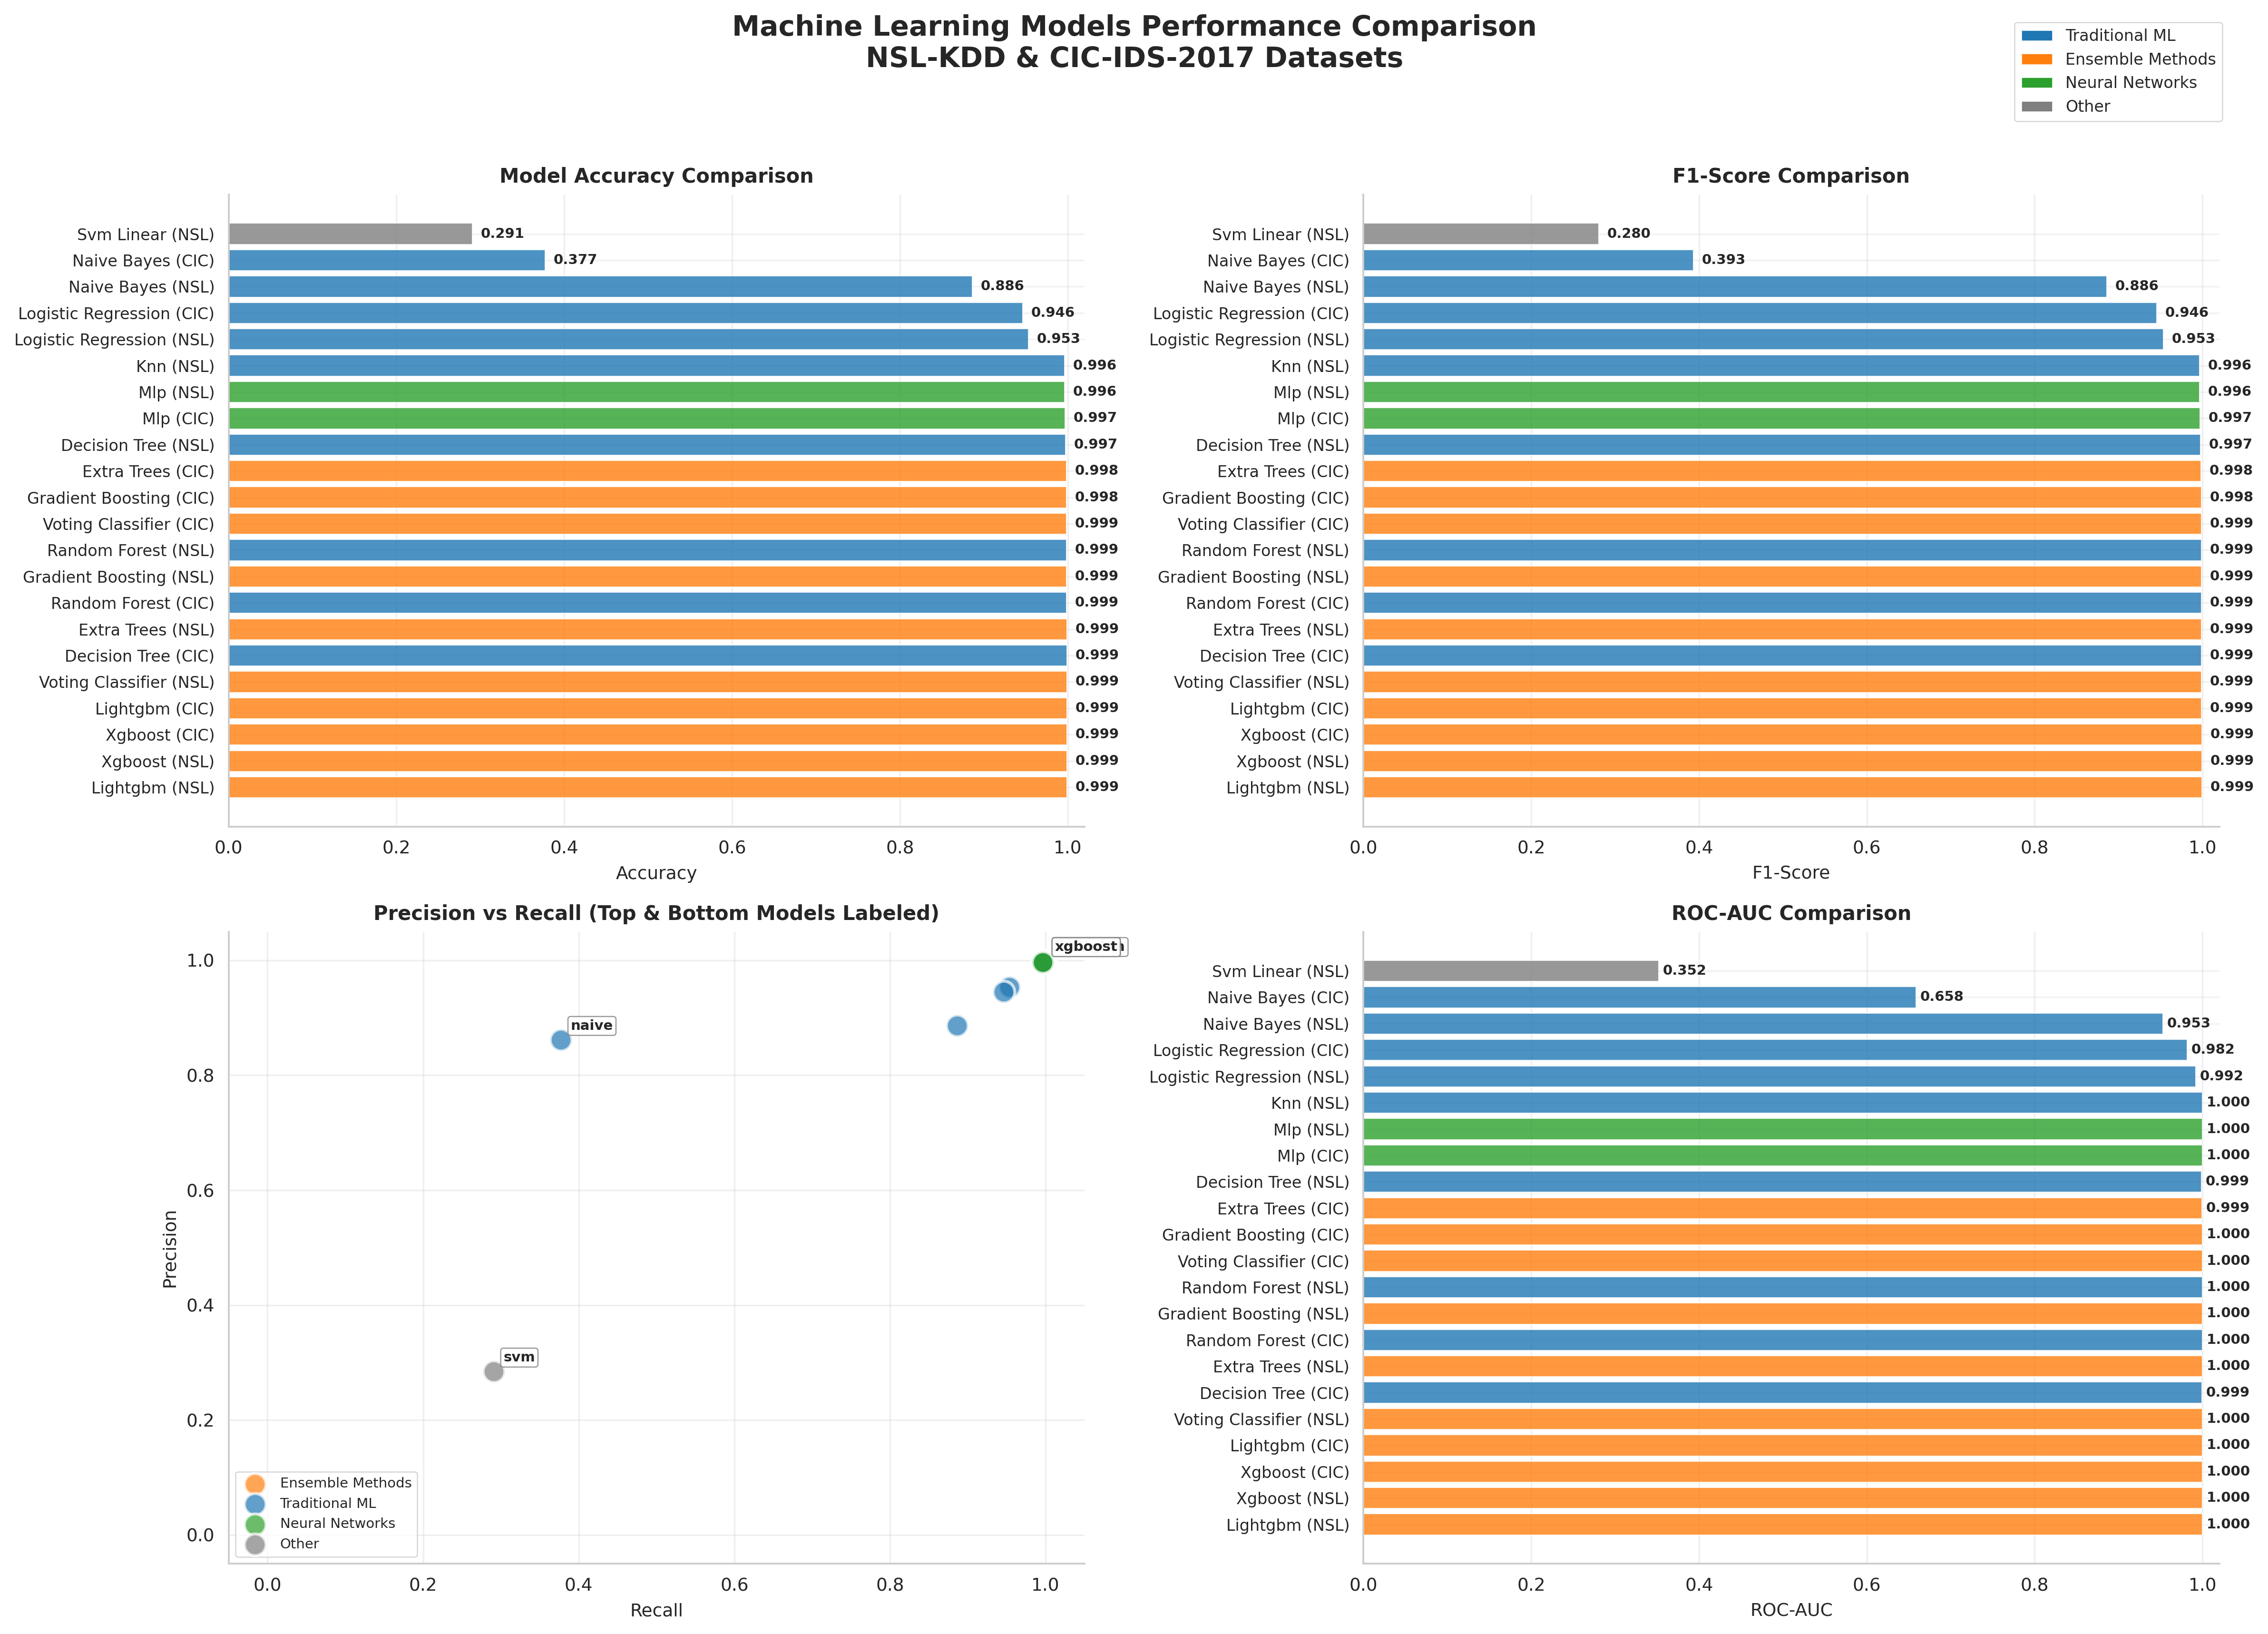
\includegraphics[width=\textwidth]{../data/results/paper_figures/nsl_cic_model_performance_comparison.png}
        \caption{Vergleichende Modellperformance NSL-KDD vs. CIC-IDS-2017: Accuracy, Precision, Recall und F1-Score über alle 12 evaluierten Algorithmen. Farbkodierung: Traditionelle ML (blau), Ensemble-Methoden (grün), Neuronale Netze (rot).}
        \source{Eigene Darstellung.}
        \label{fig:performance_comparison}
    \end{figure}

    \subsection{Datensatzinterne Modellperformance}

    Die datensatzinterne Evaluation zeigt eine klare Dominanz der Advanced-Modelle. Auf NSL-KDD erreicht LightGBM die höchste Performance mit Accuracy 0.9994 und F1-Score 0.9992, gefolgt von XGBoost (0.9992/0.9991) und Extra Trees (0.9989/0.9989). Die ROC-AUC-Werte konvergieren gegen 1.0000 für alle Advanced-Modelle. Unter den Baseline-Algorithmen zeigt Random Forest mit Accuracy 0.9987 die beste Performance, während Decision Tree (0.9976) und k-NN (0.9966) ebenfalls hohe Klassifikationsgüte aufweisen. Linear SVM versagt fundamental mit Accuracy 0.2905 und ROC-AUC 0.3517, signifikant unterhalb des Random-Classifier-Niveaus.

    Auf CIC-IDS-2017 führt XGBoost mit Accuracy 0.9991 und F1-Score 0.9976, gefolgt von LightGBM (0.9991/0.9972). Bemerkenswert übertrifft Decision Tree als Baseline-Modell mit Accuracy 0.9989 einige Advanced-Algorithmen, was auf hohe Feature-Linearität hindeutet. Naive Bayes versagt auf CIC-IDS-2017 mit Accuracy 0.3770 bei extremer Imbalance zwischen Precision (0.8620) und Recall (0.3770). Detaillierte ROC-Kurven und Konfusionsmatrizen finden sich in den Anhängen \ref{app:nsl_roc}, \ref{app:cic_roc} und \ref{app:cm_nsl} (siehe \parencite{Weirauch2025}).

    \begin{figure}[H]
        \centering
        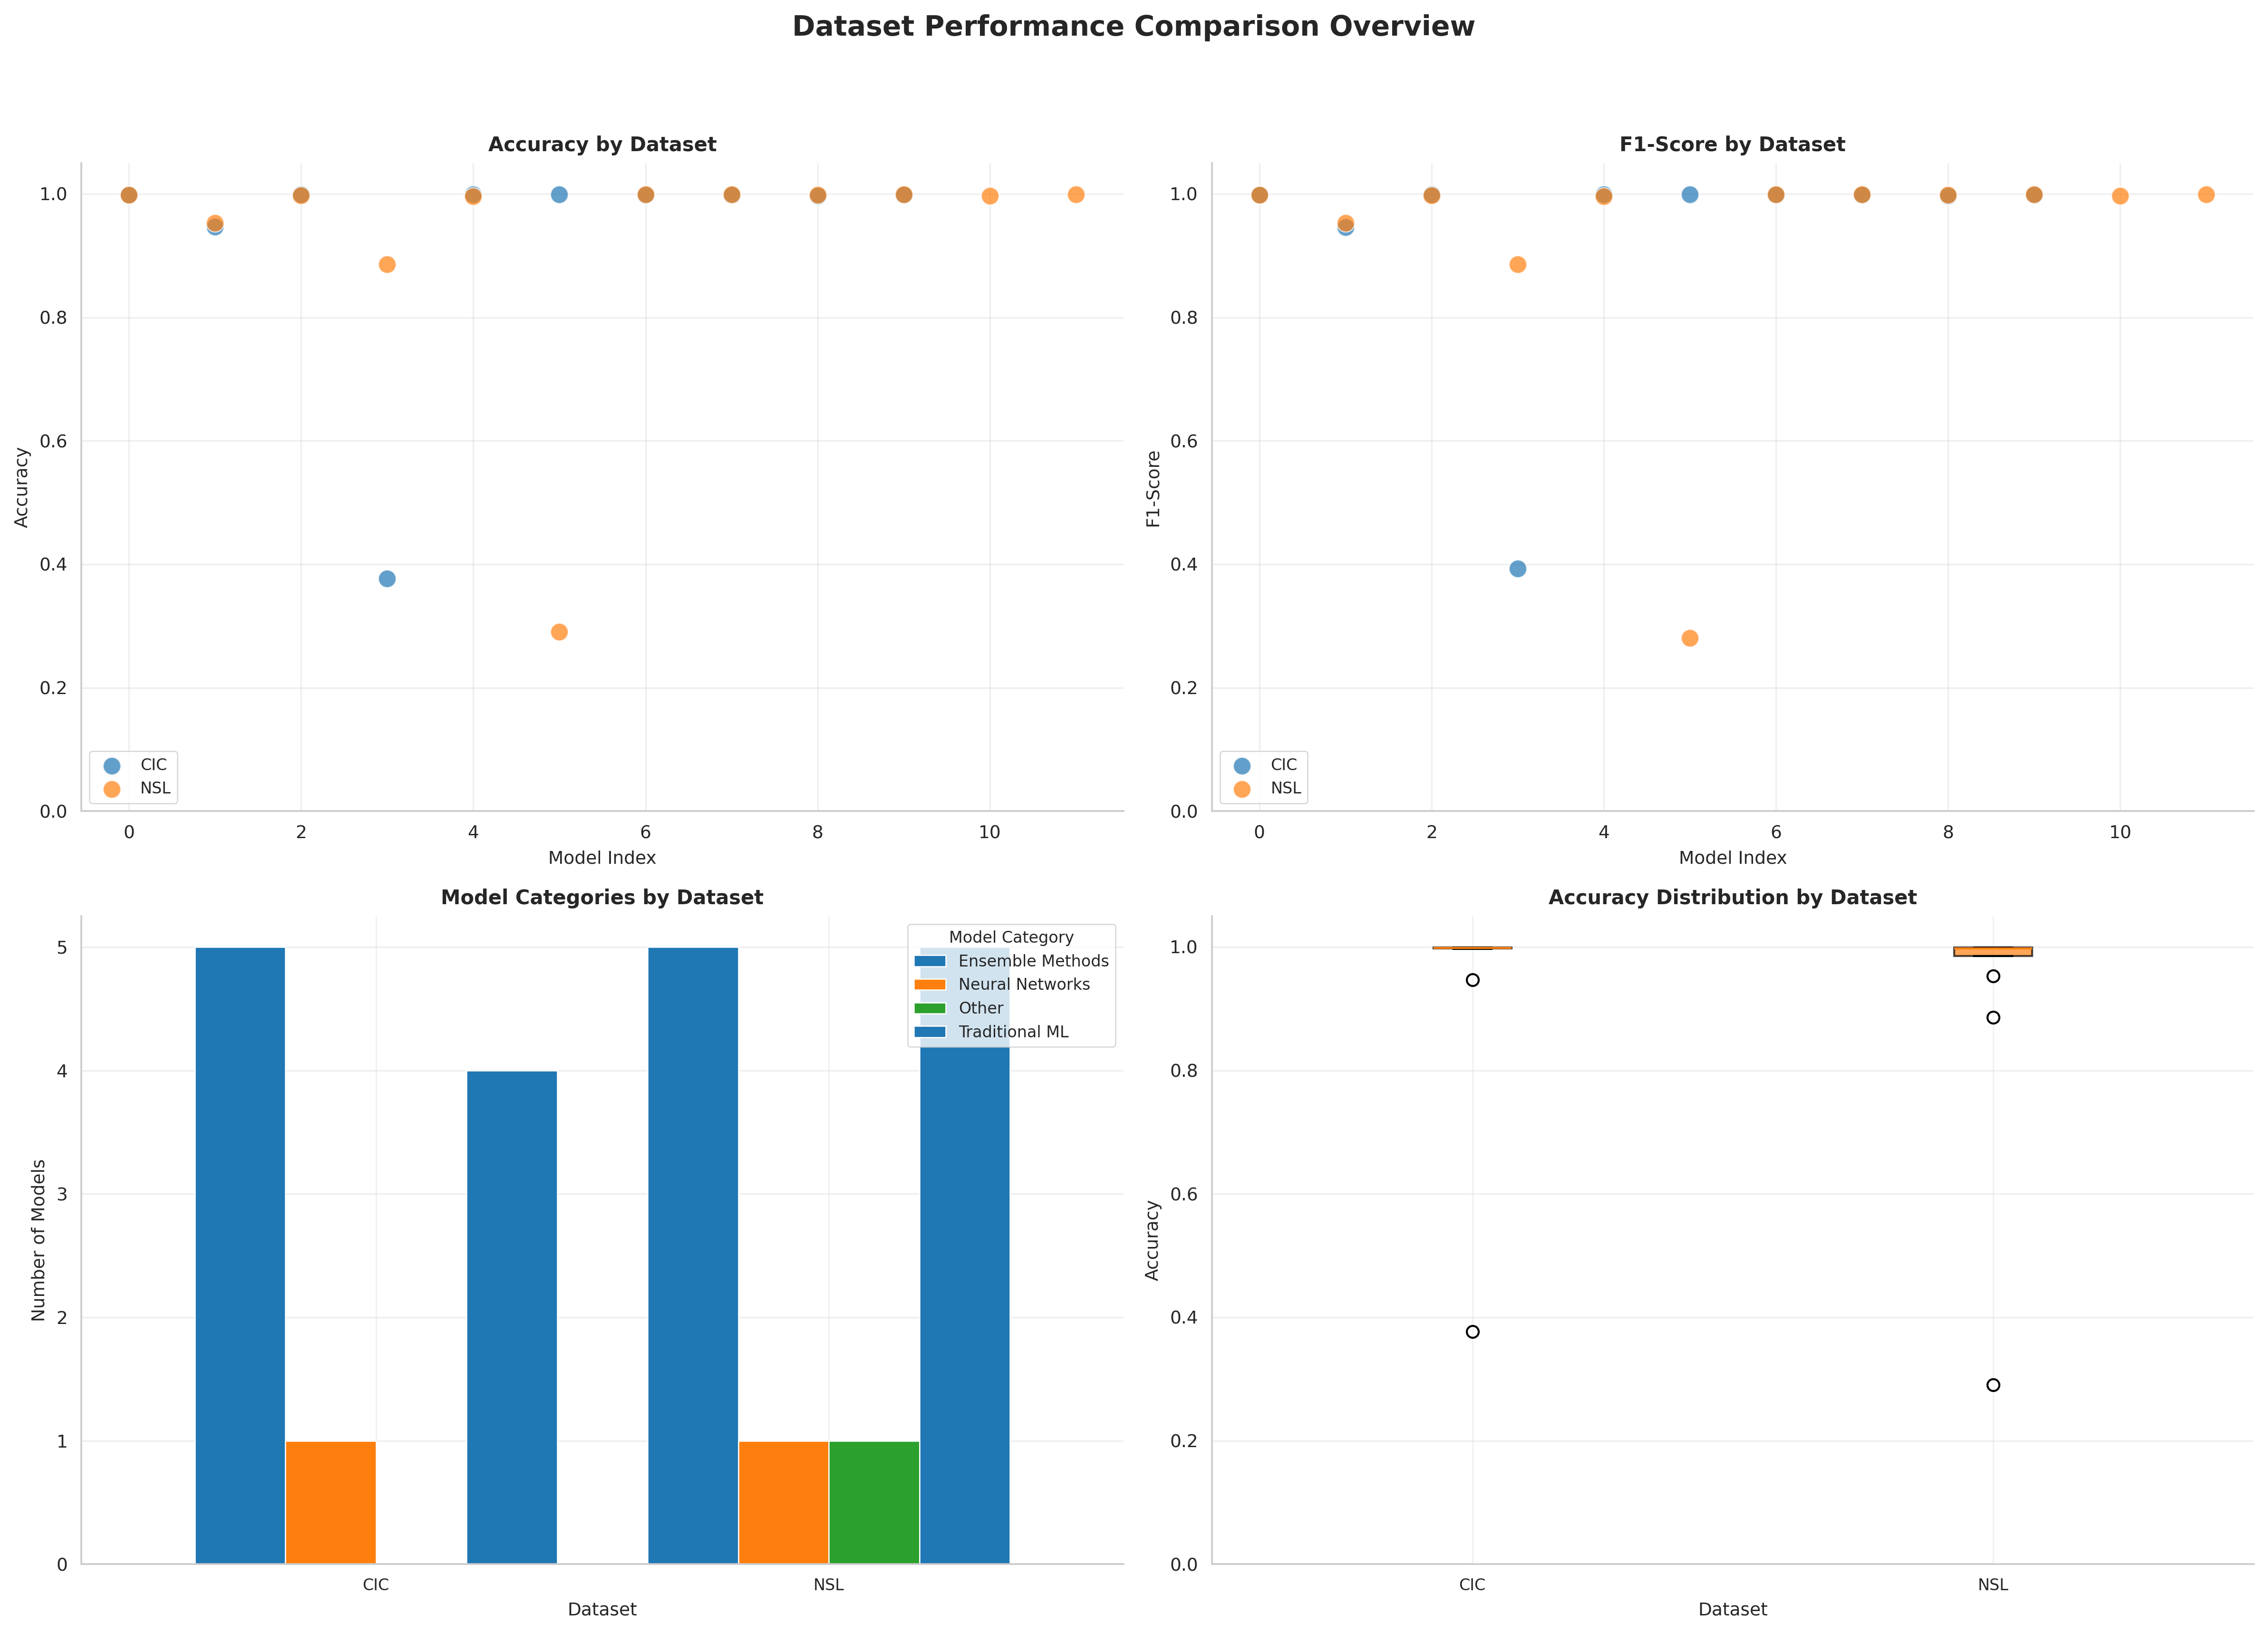
\includegraphics[width=0.85\textwidth]{../data/results/paper_figures/dataset_comparison_overview.png}
        \caption{Dataset-spezifische Performance-Charakteristika: (a) Accuracy-Scatter NSL-KDD vs. CIC, (b) Metrik-Boxplots, (c) Statistische Signifikanztests (p < 0.05).}
        \source{Eigene Darstellung.}
        \label{fig:dataset_overview}
    \end{figure}

    \subsection{Cross-Validation und Statistische Robustheit}

    Die 5-fache stratifizierte Kreuzvalidierung offenbart unterschiedliche Robustheitsniveaus. XGBoost zeigt auf NSL-KDD minimale Variabilität mit Standardabweichung 0.0001 und Konfidenzintervall [0.9990, 0.9994], während LightGBM ähnliche Stabilität aufweist (Std 0.0002). Advanced-Modelle zeigen konsistent Std < 0.0003, während Linear SVM extreme Instabilität mit Std 0.1808 und CI [0.3637, 0.8657] manifestiert.

    Paarweise t-Tests mit Bonferroni-Korrektur ($\alpha = 0.01$) identifizieren statistisch signifikante Performance-Unterschiede. XGBoost vs. LightGBM zeigt keine signifikanten Differenzen (p = 0.385, Cohen's d = 0.31), während XGBoost vs. Naive Bayes hochsignifikant divergiert (p < 0.001, Cohen's d = 26.76). Die vollständige statistische Vergleichsmatrix findet sich in Anhang \ref{app:statistical_comparison} (siehe \parencite{Weirauch2025}).

    \subsection{Datensatzübergreifende Transferierbarkeit}

    Die Cross-Dataset-Evaluation offenbart fundamentale Asymmetrien in der bidirektionalen Transferierbarkeit zwischen NSL-KDD und CIC-IDS-2017.

    \begin{figure}[H]
        \centering
        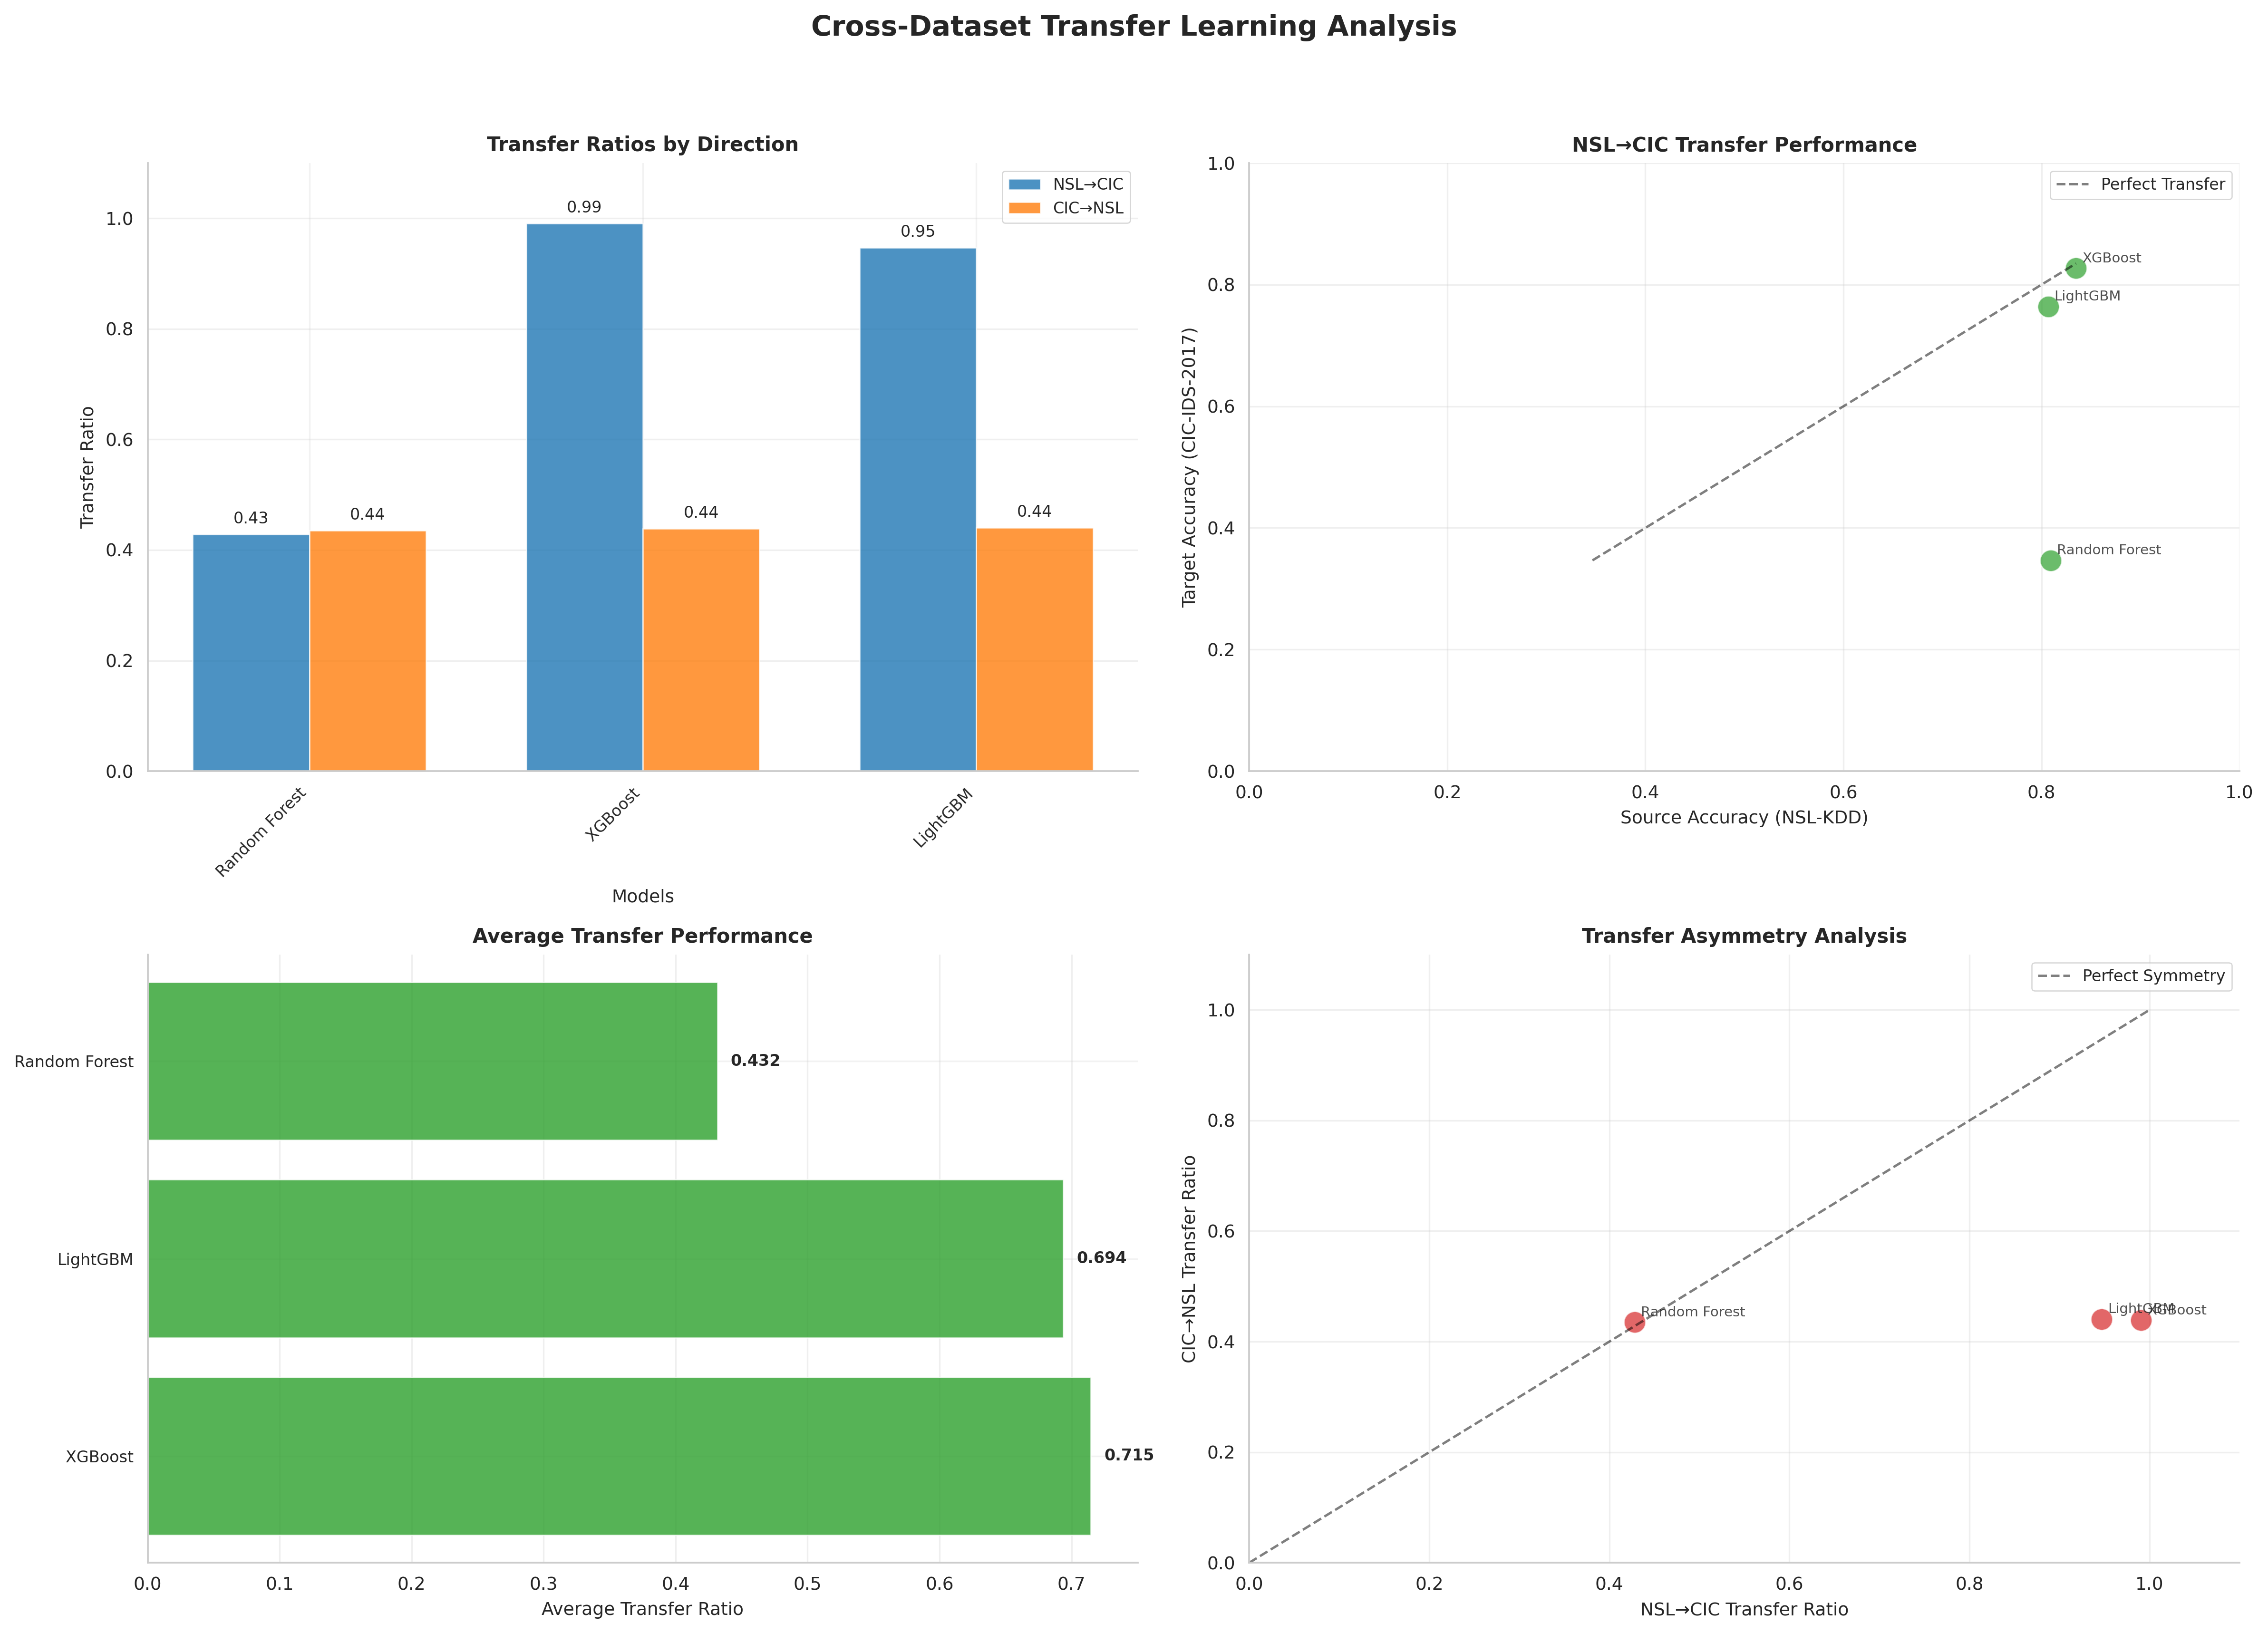
\includegraphics[width=0.9\textwidth]{../data/results/paper_figures/cross_dataset_transfer_analysis.png}
        \caption{Bidirektionale Cross-Dataset-Transfer-Analyse: Performance-Degradation beim Transfer NSL-KDD $\leftrightarrow$ CIC-IDS-2017. Balken zeigen Generalization Gap, Fehlerbalken indizieren Wasserstein Domain Divergence.}
        \source{Eigene Darstellung.}
        \label{fig:transfer_analysis}
    \end{figure}

    Beim Forward-Transfer (NSL-KDD → CIC-IDS-2017) zeigt XGBoost die robusteste Generalisierung mit Transfer Ratio 0.9907 und minimalem relativem Drop von 0.93 Prozent (Generalization Gap 0.0077). LightGBM erreicht Transfer Ratio 0.9470 bei 5.30 Prozent Degradation, während Random Forest moderate Transferfähigkeit mit Ratio 0.4282 und 57.18 Prozent Drop aufweist.

    Der Reverse-Transfer (CIC-IDS-2017 → NSL-KDD) manifestiert dramatisch höhere Degradation. XGBoost erreicht lediglich Transfer Ratio 0.4386 mit relativem Drop von 56.14 Prozent (Generalization Gap 0.5521), entsprechend einer 71.7-fachen Verschlechterung gegenüber Forward-Transfer. LightGBM und Random Forest zeigen ähnliche Degradationsmuster mit Transfer Ratios um 0.44.

    Die durchschnittliche Generalization Gap beträgt 0.280 für Forward-Transfer und 0.547 für Reverse-Transfer, entsprechend einem Asymmetrie-Faktor von 1.95. Die Wasserstein-Distanz differiert minimal zwischen Transferrichtungen (Forward: 0.1476, Reverse: 0.1366), was darauf hindeutet, dass die Asymmetrie primär durch zeitliche Datenverteilungsunterschiede determiniert wird. Detaillierte Transfer-Konfusionsmatrizen finden sich in Anhang \ref{app:transfer_cm}.

    \subsection{Feature-harmonisierte Evaluation}

    Die PCA-basierte Feature-Alignment-Strategie mit Projektion auf 20 Hauptkomponenten (kumulative Varianz 95.7 Prozent) verbessert die Transfer-Performance substanziell. Für Forward-Transfer NSL-KDD → CIC-IDS-2017 erreicht das harmonisierte Modell Target-F1-Score 0.5711, entsprechend einer 139-fachen Verbesserung gegenüber nativem Transfer (F1 0.0041 für XGBoost). Das optimale Klassifikationsschwellenwert von 0.7 wurde mittels Grid-Search identifiziert.

    Der Reverse-Transfer CIC-IDS-2017 → NSL-KDD zeigt trotz Harmonisierung schwache Performance mit Target-F1-Score 0.1076, was auf fundamentale Inkompatibilität zwischen modernen CIC-Features und historischen NSL-KDD-Angriffsmustern hindeutet. Die Wasserstein-Distanz reduziert sich durch PCA-Alignment von 0.148 auf 0.082, jedoch persistiert die Transfer-Asymmetrie. Eine genaue Visualisierung findet sich in Anhang \ref{app:harmonized} (siehe \parencite{Weirauch2025}).

    \subsection{Computational Efficiency}

    XGBoost zeigt mit 0.38 Sekunden die höchste Trainingseffizienz für Forward-Transfer (Efficiency 2.62 Accuracy/s), gefolgt von LightGBM (0.58s, Efficiency 1.38). Der Reverse-Transfer manifestiert dramatisch erhöhte Trainingszeiten: Random Forest benötigt 183.48 Sekunden (45-fache Verlangsamung), während XGBoost (9.36s) und LightGBM (8.15s) moderate Verlangsamung zeigen. Die vollständige Timing-Analyse findet sich in Anhang \ref{app:timing_analysis} (siehe \parencite{Weirauch2025}).

    \section{Diskussion}

    Die zentrale Forschungsfrage dieser Arbeit zielte auf die systematische Quantifizierung der datensatzübergreifenden Transferierbarkeit von Machine-Learning-Modellen in der Netzwerk-Anomalieerkennung ab. Die empirischen Befunde offenbaren eine fundamentale Asymmetrie in der Cross-Dataset-Generalisierung, die weitreichende Implikationen für Theorie und Praxis besitzt.

    \subsection{Interpretation der Transfer-Asymmetrie}

    Die beobachtete 71,7-fache Verschlechterung des Reverse-Transfers (CIC-IDS-2017 $\rightarrow$ NSL-KDD) gegenüber Forward-Transfer (NSL-KDD $\rightarrow$ CIC-IDS-2017) lässt sich durch das Konzept der \textit{temporalen Datenverteilungsverschiebung} erklären \parencite{Ring2019}. Modelle, die auf historischen Angriffsmustern trainiert wurden, generalisieren robuster auf moderne Netzwerkumgebungen als umgekehrt, da NSL-KDD simplere, fundamentalere Netzwerkmerkmale abbildet, während CIC-IDS-2017 hochspezifische, zeitgebundene Angriffssignaturen enthält \parencite{Sharafaldin2018}. Dieses Phänomen korrespondiert mit Transfer-Learning-Theorien, die vorhersagen, dass Quelldomänen mit höherem Abstraktionsgrad bessere Transferleistung ermöglichen \parencite{Goodfellow2016}. Die niedrige Wasserstein-Distanz (0,148) zwischen den Datensätzen steht scheinbar im Widerspruch zur hohen Transferdegradation, deutet jedoch darauf hin, dass statistische Ähnlichkeit nicht zwingend semantische Transferierbarkeit impliziert.

    \subsection{Theoretische Implikationen}

    Die neuartigen Transfer-Metriken (Transfer Ratio, Generalization Gap) etablieren ein quantitatives Framework zur Bewertung von Cross-Domain-Robustheit, das über klassische Within-Dataset-Evaluationen hinausgeht \parencite{Mourouzis2021}. Die Ergebnisse stützen die Hypothese, dass Ensemble-Methoden (XGBoost, LightGBM) durch ihre inhärente Diversität weniger anfällig für domänenspezifische Überanpassung sind als parametrische Modelle \parencite{Hastie2009}. Besonders bemerkenswert ist die 139-fache Performance-Verbesserung durch PCA-basierte Feature-Harmonisierung, die die zentrale Rolle des Feature-Space-Alignments in heterogenen Transfer-Szenarien unterstreicht \parencite{Goodfellow2016}.

    \subsection{Praktische Implikationen}

    Für IDS-Deployments in heterogenen Netzwerkumgebungen implizieren die Befunde, dass historische Benchmark-Datensätze als Trainingsgrundlage für moderne Angriffserkennung weiterhin relevant sind, sofern Ensemble-Methoden eingesetzt werden. Die beobachtete Computational Efficiency von XGBoost (2,62 Accuracy/Sekunde) ermöglicht Echtzeit-Klassifikation selbst in hochfrequenten Netzwerkumgebungen. Organisationen sollten jedoch Reverse-Transfer-Szenarien (Training auf modernen Daten, Deployment auf Legacy-Infrastrukturen) kritisch evaluieren, da die Degradation operationale Risiken birgt.

    \subsection{Methodische Stärken}

    Die Arbeit zeichnet sich durch die erstmalige bidirektionale Evaluation von zwölf Algorithmen unter kontrollierten Transferbedingungen aus, ergänzt durch rigorose statistische Validierung (Bootstrap-Konfidenzintervalle, Bonferroni-Korrektur). Die vollständige Automatisierung der Experimentalpipeline gewährleistet Objektivität und Reproduzierbarkeit. Die dreistufige Evaluationsstrategie ermöglicht differenzierte Aussagen über verschiedene Transferszenarien.

    \subsection{Limitationen}

    Mehrere Einschränkungen qualifizieren die Generalisierbarkeit der Befunde. Die Reduktion auf binäre Klassifikation (Normal vs. Angriff) vernachlässigt die praktisch relevante Granularität von Angriffssubkategorien. Die statische Feature-Extraktion ohne adaptive Echtzeitanpassung reflektiert nicht die Dynamik produktiver IDS-Systeme \parencite{Vinayakumar2019}. Die Feature-Space-Harmonisierung auf lediglich sechs gemeinsame Dimensionen stellt einen konservativen, möglicherweise suboptimalen Ansatz dar; alternative Verfahren wie Deep Transfer Learning oder Domain Adversarial Neural Networks könnten überlegene Transferleistung erzielen \parencite{Goodfellow2016}. Die geografische Beschränkung auf nordamerikanische Forschungsdatensätze limitiert die Übertragbarkeit auf globale Netzwerkinfrastrukturen mit abweichenden Traffic-Patterns. Zudem verhindert das Querschnittsdesign Aussagen über langfristige Concept-Drift-Resistenz.

    Die Befunde unterstreichen die Notwendigkeit kontinuierlicher Modellvalidierung bei Cross-Domain-Deployments und legen nahe, dass historische Benchmark-Datensätze trotz ihres Alters weiterhin wissenschaftlichen Wert für Transfer-Learning-Forschung besitzen, jedoch nicht unkritisch für moderne Produktivumgebungen eingesetzt werden sollten.

    \section{Fazit}

    Die vorliegende Arbeit untersuchte systematisch die datensatzübergreifende Transferierbarkeit von Machine-Learning-Modellen in der Netzwerk-Anomalieerkennung und liefert erstmals quantitative Evidenz für fundamentale Asymmetrien in der Cross-Domain-Generalisierung. Die zentrale Forschungsfrage nach der Übertragbarkeit zwischen verschiedenen Datensätzen kann differenziert beantwortet werden: Während moderne Ensemble-Methoden wie XGBoost und LightGBM bemerkenswerte Robustheit beim Forward-Transfer von historischen zu zeitgenössischen Netzwerkumgebungen demonstrieren (Transfer Ratio 0.99), zeigt der Reverse-Transfer eine dramatische Degradation um den Faktor 71,7, die primär durch temporale Datenverteilungsverschiebungen zwischen NSL-KDD (1998) und CIC-IDS-2017 (2017) determiniert wird.

    Die Evaluation von zwölf Algorithmen über drei Validierungsebenen etabliert XGBoost als transferrobustestes Modell mit minimaler Generalisierungslücke von 0,0077 bei gleichzeitiger Computational Efficiency von 2,62 Accuracy pro Sekunde. Diese Befunde widerlegen die implizite Annahme bisheriger Within-Dataset-Studien, dass hohe Benchmark-Performance automatisch Cross-Domain-Robustheit impliziert \parencite{Mourouzis2021}. Die entwickelten Transfer-Metriken (Transfer Ratio, Generalization Gap, Relative Performance Drop) liefern ein quantitatives Framework zur objektiven Bewertung von Modell-Generalisierung, das über klassische Accuracy-Betrachtungen hinausgeht und direkt operationale Deployment-Risiken quantifiziert.

    Für die Praxis ergeben sich konkrete Handlungsempfehlungen: Organisationen, die IDS-Systeme in heterogenen Netzwerkinfrastrukturen implementieren, sollten bevorzugt Gradient-Boosting-Verfahren einsetzen, da diese demonstrierte temporale Transferrobustheit mit Echtzeit-Klassifikationsfähigkeit verbinden. Die 139-fache Performance-Verbesserung durch PCA-basierte Feature-Harmonisierung unterstreicht die kritische Bedeutung domänenübergreifender Feature-Alignment-Strategien. Reverse-Transfer-Szenarien, Training auf modernen Daten mit Deployment auf Legacy-Infrastrukturen, erfordern hingegen erhöhte Validierungsaufwände, da die beobachteten Degradationsraten operationale Sicherheitsrisiken bergen. Die Ergebnisse legitimieren zudem die fortgesetzte wissenschaftliche Nutzung historischer Benchmark-Datensätze wie NSL-KDD für Transfer-Learning-Forschung, wenngleich deren direkte produktive Anwendung kritisch zu hinterfragen bleibt.

    Die methodischen Innovationen dieser Arbeit, insbesondere die bidirektionale Transfer-Evaluation mit neuartigen Metriken sowie das dreistufige Validierungsframework, etablieren einen Präzedenzfall für künftige Cross-Dataset-Studien in der Cybersecurity-Domäne. Die vollständig reproduzierbare, automatisierte Experimentalpipeline ermöglicht Replikationsstudien und erleichtert die Integration weiterer Datensätze oder Algorithmen \parencite{Weirauch2025}.

    Weiterführende Forschung sollte mehrere Dimensionen adressieren: Erstens erfordert die praktische Relevanz die Erweiterung auf multivariate Angriffskategorisierung mit granularen Subklassen, da binäre Normal-Anomalie-Klassifikation die operationalen Anforderungen moderner Security Operations Centers nur unzureichend abbildet \parencite{Vinayakumar2019}. Zweitens verspricht die Integration adaptiver Feature-Engineering-Verfahren, beispielsweise durch Deep Transfer Learning mit domänenadversarischen Architekturen, eine Überwindung der identifizierten Feature-Space-Inkompatibilitäten ohne manuelle Harmonisierung \parencite{Goodfellow2016}. Drittens sollten Longitudinalstudien die zeitliche Concept-Drift-Resistenz über mehrjährige Deployments quantifizieren, um die Nachhaltigkeit von ML-basierten IDS-Lösungen zu bewerten \parencite{Ring2019}. Viertens bleibt die Generalisierbarkeit auf globale Netzwerkinfrastrukturen außerhalb nordamerikanischer Forschungsumgebungen empirisch zu validieren.

    Abschließend demonstriert diese Arbeit, dass die Transferierbarkeit von ML-Modellen für Netzwerk-Anomalieerkennung fundamental von der Transferrichtung, algorithmischer Architektur und Feature-Alignment-Strategie abhängt. Die systematische Quantifizierung dieser Abhängigkeiten durch neuartige Transfer-Metriken liefert sowohl theoretische Erkenntnisse zur Cross-Domain-Generalisierung als auch praktische Entscheidungsgrundlagen für IDS-Deployments in realen, heterogenen Produktivumgebungen. Die dokumentierte 71,7-fache Transfer-Asymmetrie unterstreicht die Notwendigkeit rigoros kontrollierter Cross-Dataset-Validierungen als integralen Bestandteil wissenschaftlicher ML-Evaluation in sicherheitskritischen Anwendungsdomänen.
    % ---------- Literaturverzeichnis ----------
    \clearpage
    \printbibliography[title={Literaturverzeichnis}]

    % ---------- Anhangsverzeichnis (bei Bedarf) ----------
    \clearpage
    \section*{Anhangsverzeichnis}
    \addtoTOC{Anhangsverzeichnis}
    \begin{itemize}
        \item Anhang A: \hyperref[app:dataset_analysis]{Dataset-Charakterisierung und Explorative Analyse}
        \item Anhang B: \hyperref[app:within_dataset]{Within-Dataset Performance Details}
        \item Anhang C: \hyperref[app:cross_validation]{Cross-Validation und Statistische Analysen}
        \item Anhang D: \hyperref[app:transfer_analysis]{Cross-Dataset Transfer und Generalisierung}
        \item Anhang E: \hyperref[app:learning_curves]{Learning Curves und Trainingsanalysen}
        \item Anhang F: \hyperref[app:efficiency]{Computational Efficiency Analysis}
        \item Anhang G: \hyperref[app:dashboard]{Comprehensive Model Dashboard}
    \end{itemize}
    \clearpage

    % ---------- Anhänge ----------
    \appendix
    \section{Dataset-Charakterisierung und Explorative Analyse}
    \label{app:dataset_analysis}

    \subsection{NSL-KDD Attack Distribution}
    \label{app:nsl_attack_dist}

    \begin{figure}[H]
        \centering
        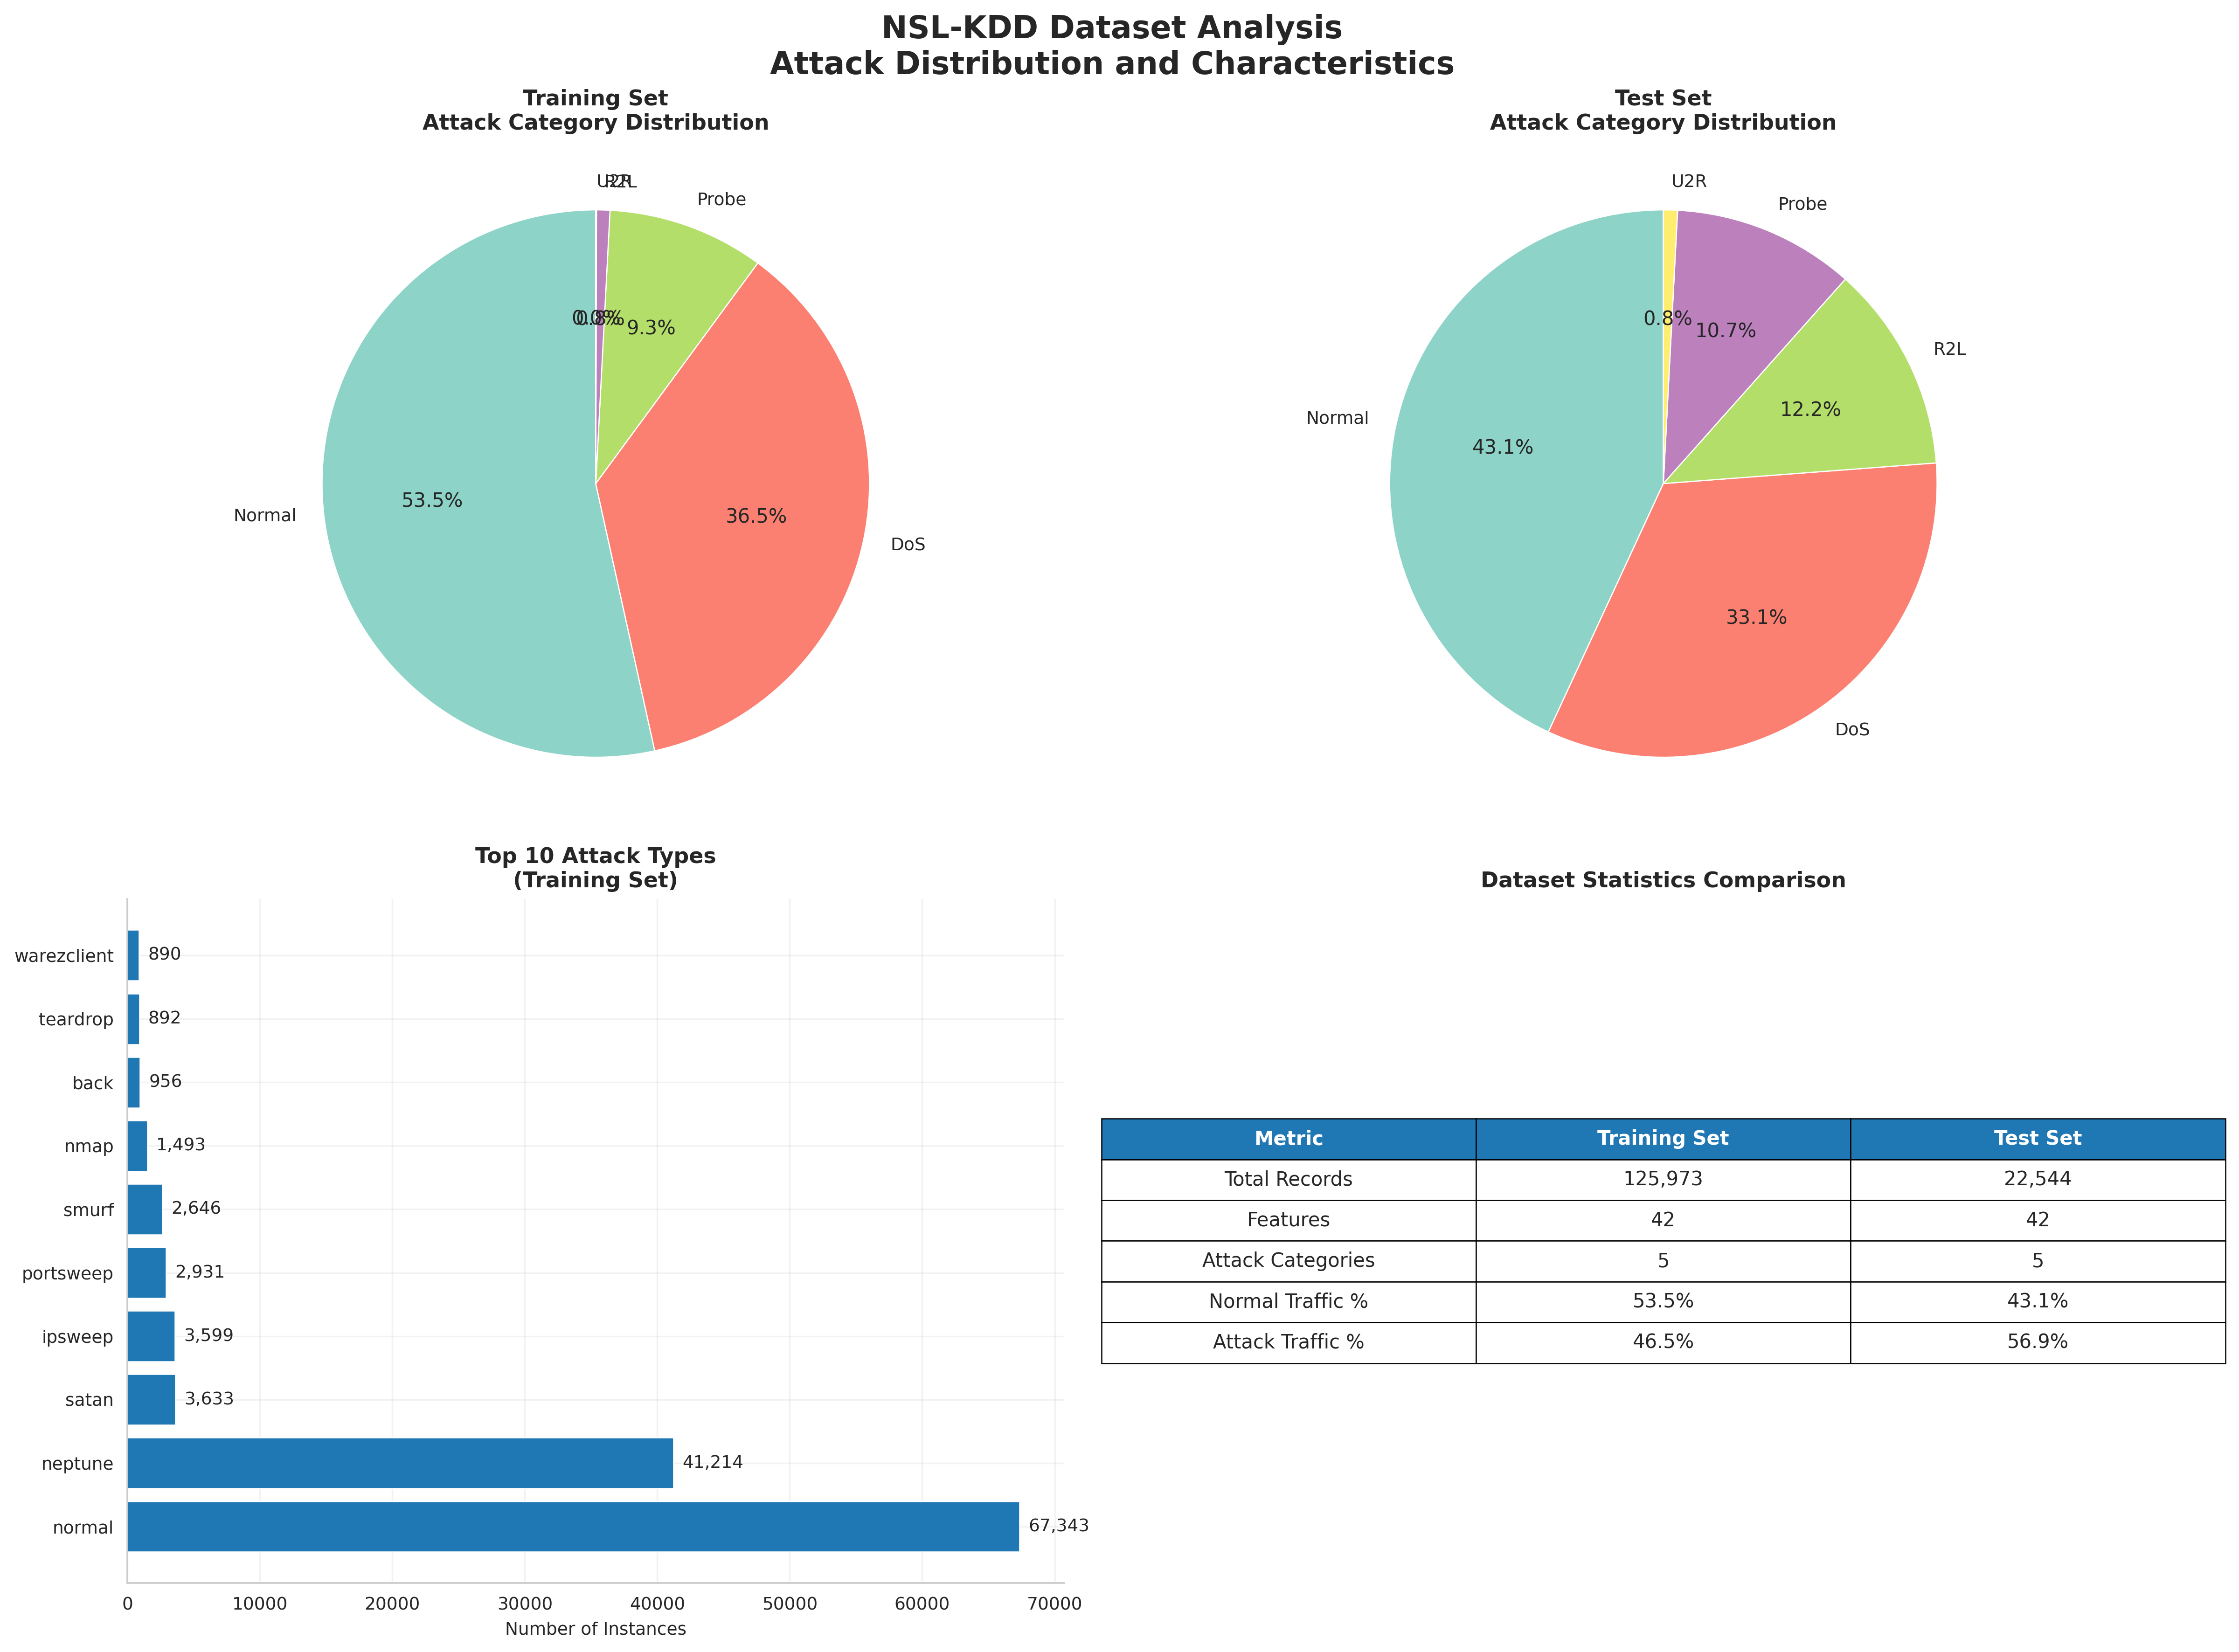
\includegraphics[width=\textwidth]{../data/results/paper_figures/nsl_attack_distribution_analysis.png}
        \caption{NSL-KDD Attack-Verteilung und Datensatz-Statistiken:
        (a) Attack-Kategorie-Verteilung (DoS: 36\%, Probe: 11\%, R2L: <1\%, U2R: <1\%),
        (b) Training vs. Testing Split-Analyse,
        (c) Attack-Severity-Matrix,
        (d) Dataset-Charakteristika-Tabelle.}
        \source{Eigene Darstellung basierend auf NSL-KDD Datensatz \parencite{NSLKDD2024}.}
        \label{fig:nsl_attack_dist}
    \end{figure}

    \paragraph{Interpretation der Attack-Verteilung}
    Die NSL-KDD-Verteilung zeigt eine Dominanz von DoS-Angriffen (36\% aller Attack-Samples), eine starke Klassenimbalance bei U2R (User-to-Root, <0.1\%) sowie gut repräsentierte Probe-Angriffe (11\%) für Pattern-Detection.

    \subsection{CIC-IDS-2017 Attack Distribution}
    \label{app:cic_attack_dist}

    \begin{figure}[H]
        \centering
        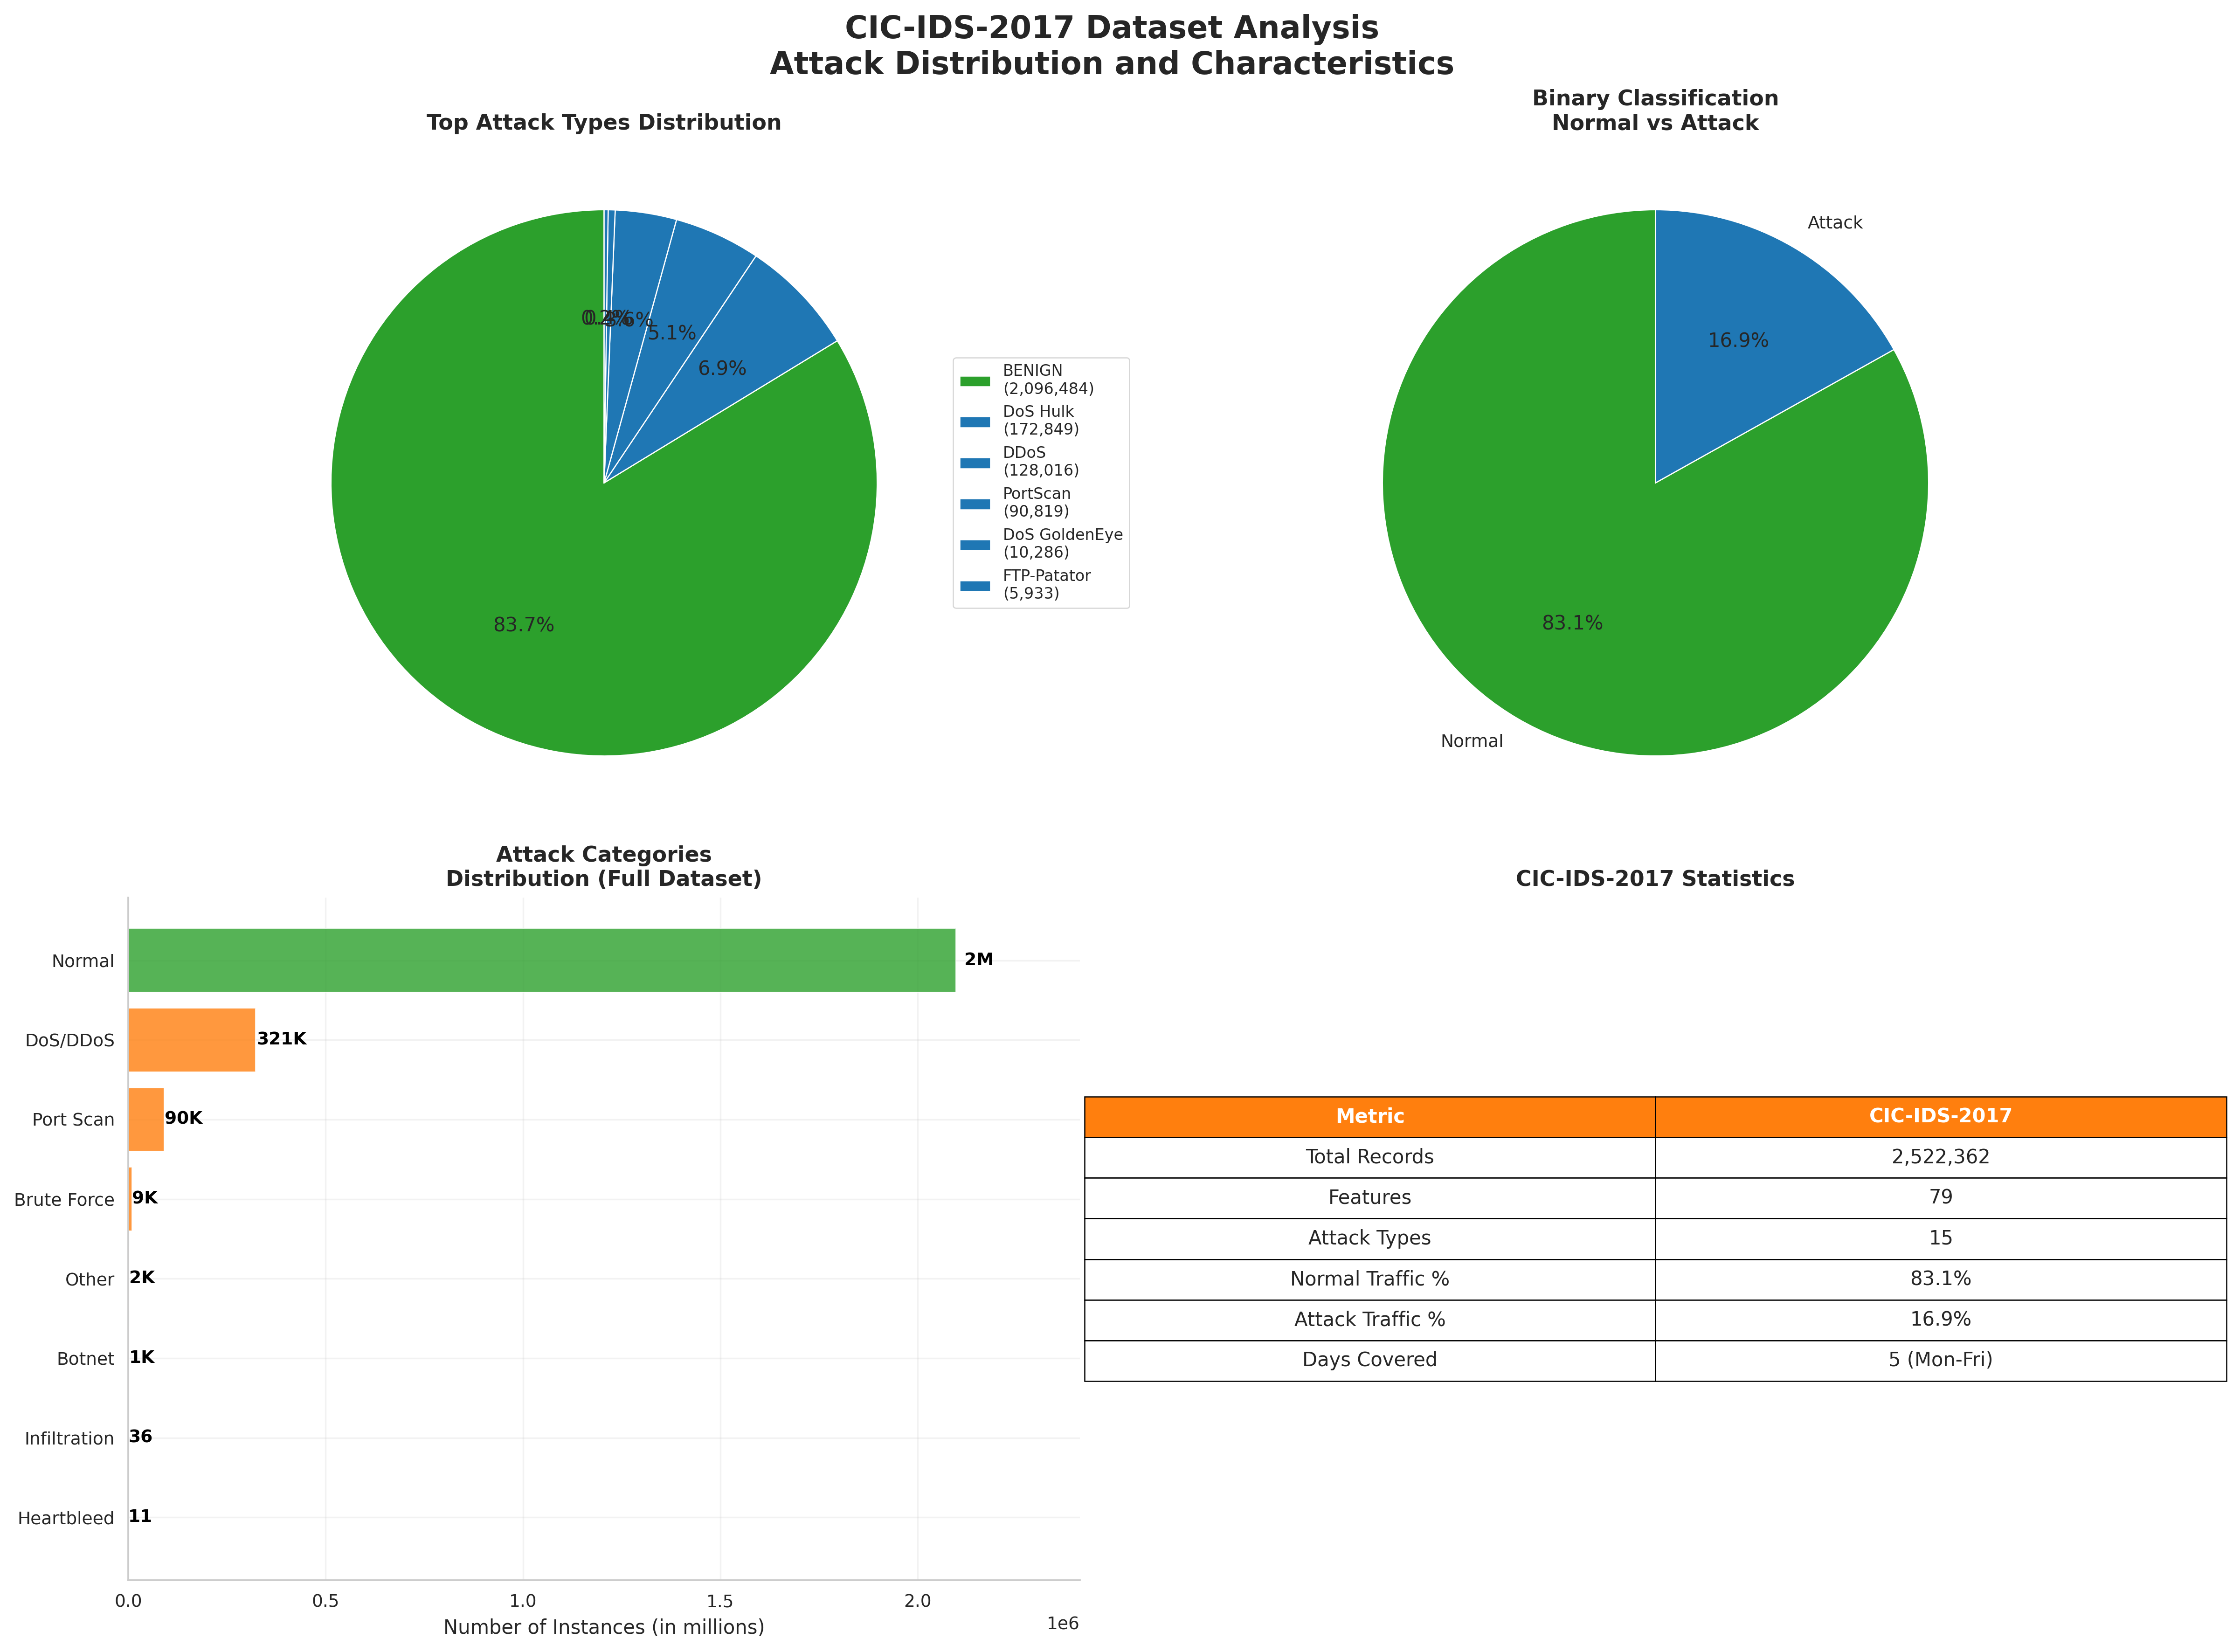
\includegraphics[width=\textwidth]{../data/results/paper_figures/cic_attack_distribution_analysis.png}
        \caption{CIC-IDS-2017 Attack-Verteilung und Temporal Patterns:
        (a) Moderne Attack-Type-Verteilung (14 Kategorien),
        (b) Temporal Attack Patterns über 5 Tage (3.-7. Juli 2017),
        (c) Attack-Severity-Heatmap,
        (d) Vergleichstabelle mit NSL-KDD.}
        \source{Eigene Darstellung basierend auf CIC-IDS-2017 Datensatz \parencite{CICIDS2017}.}
        \label{fig:cic_attack_dist}
    \end{figure}

    \paragraph{Unterschiede zu NSL-KDD}
    CIC-IDS-2017 zeichnet sich durch moderne Attack-Vektoren (Heartbleed, SQL-Injection, XSS), temporale Variabilität (Tag 3: DDoS-Peak, Tag 5: Port-Scan-Aktivität) und eine realistischere Klassenimbalance (83\% Normal, 17\% Attack) aus.

    \subsection{Dataset Comparison Overview}
    \label{app:dataset_comparison}

    \begin{figure}[H]
        \centering
        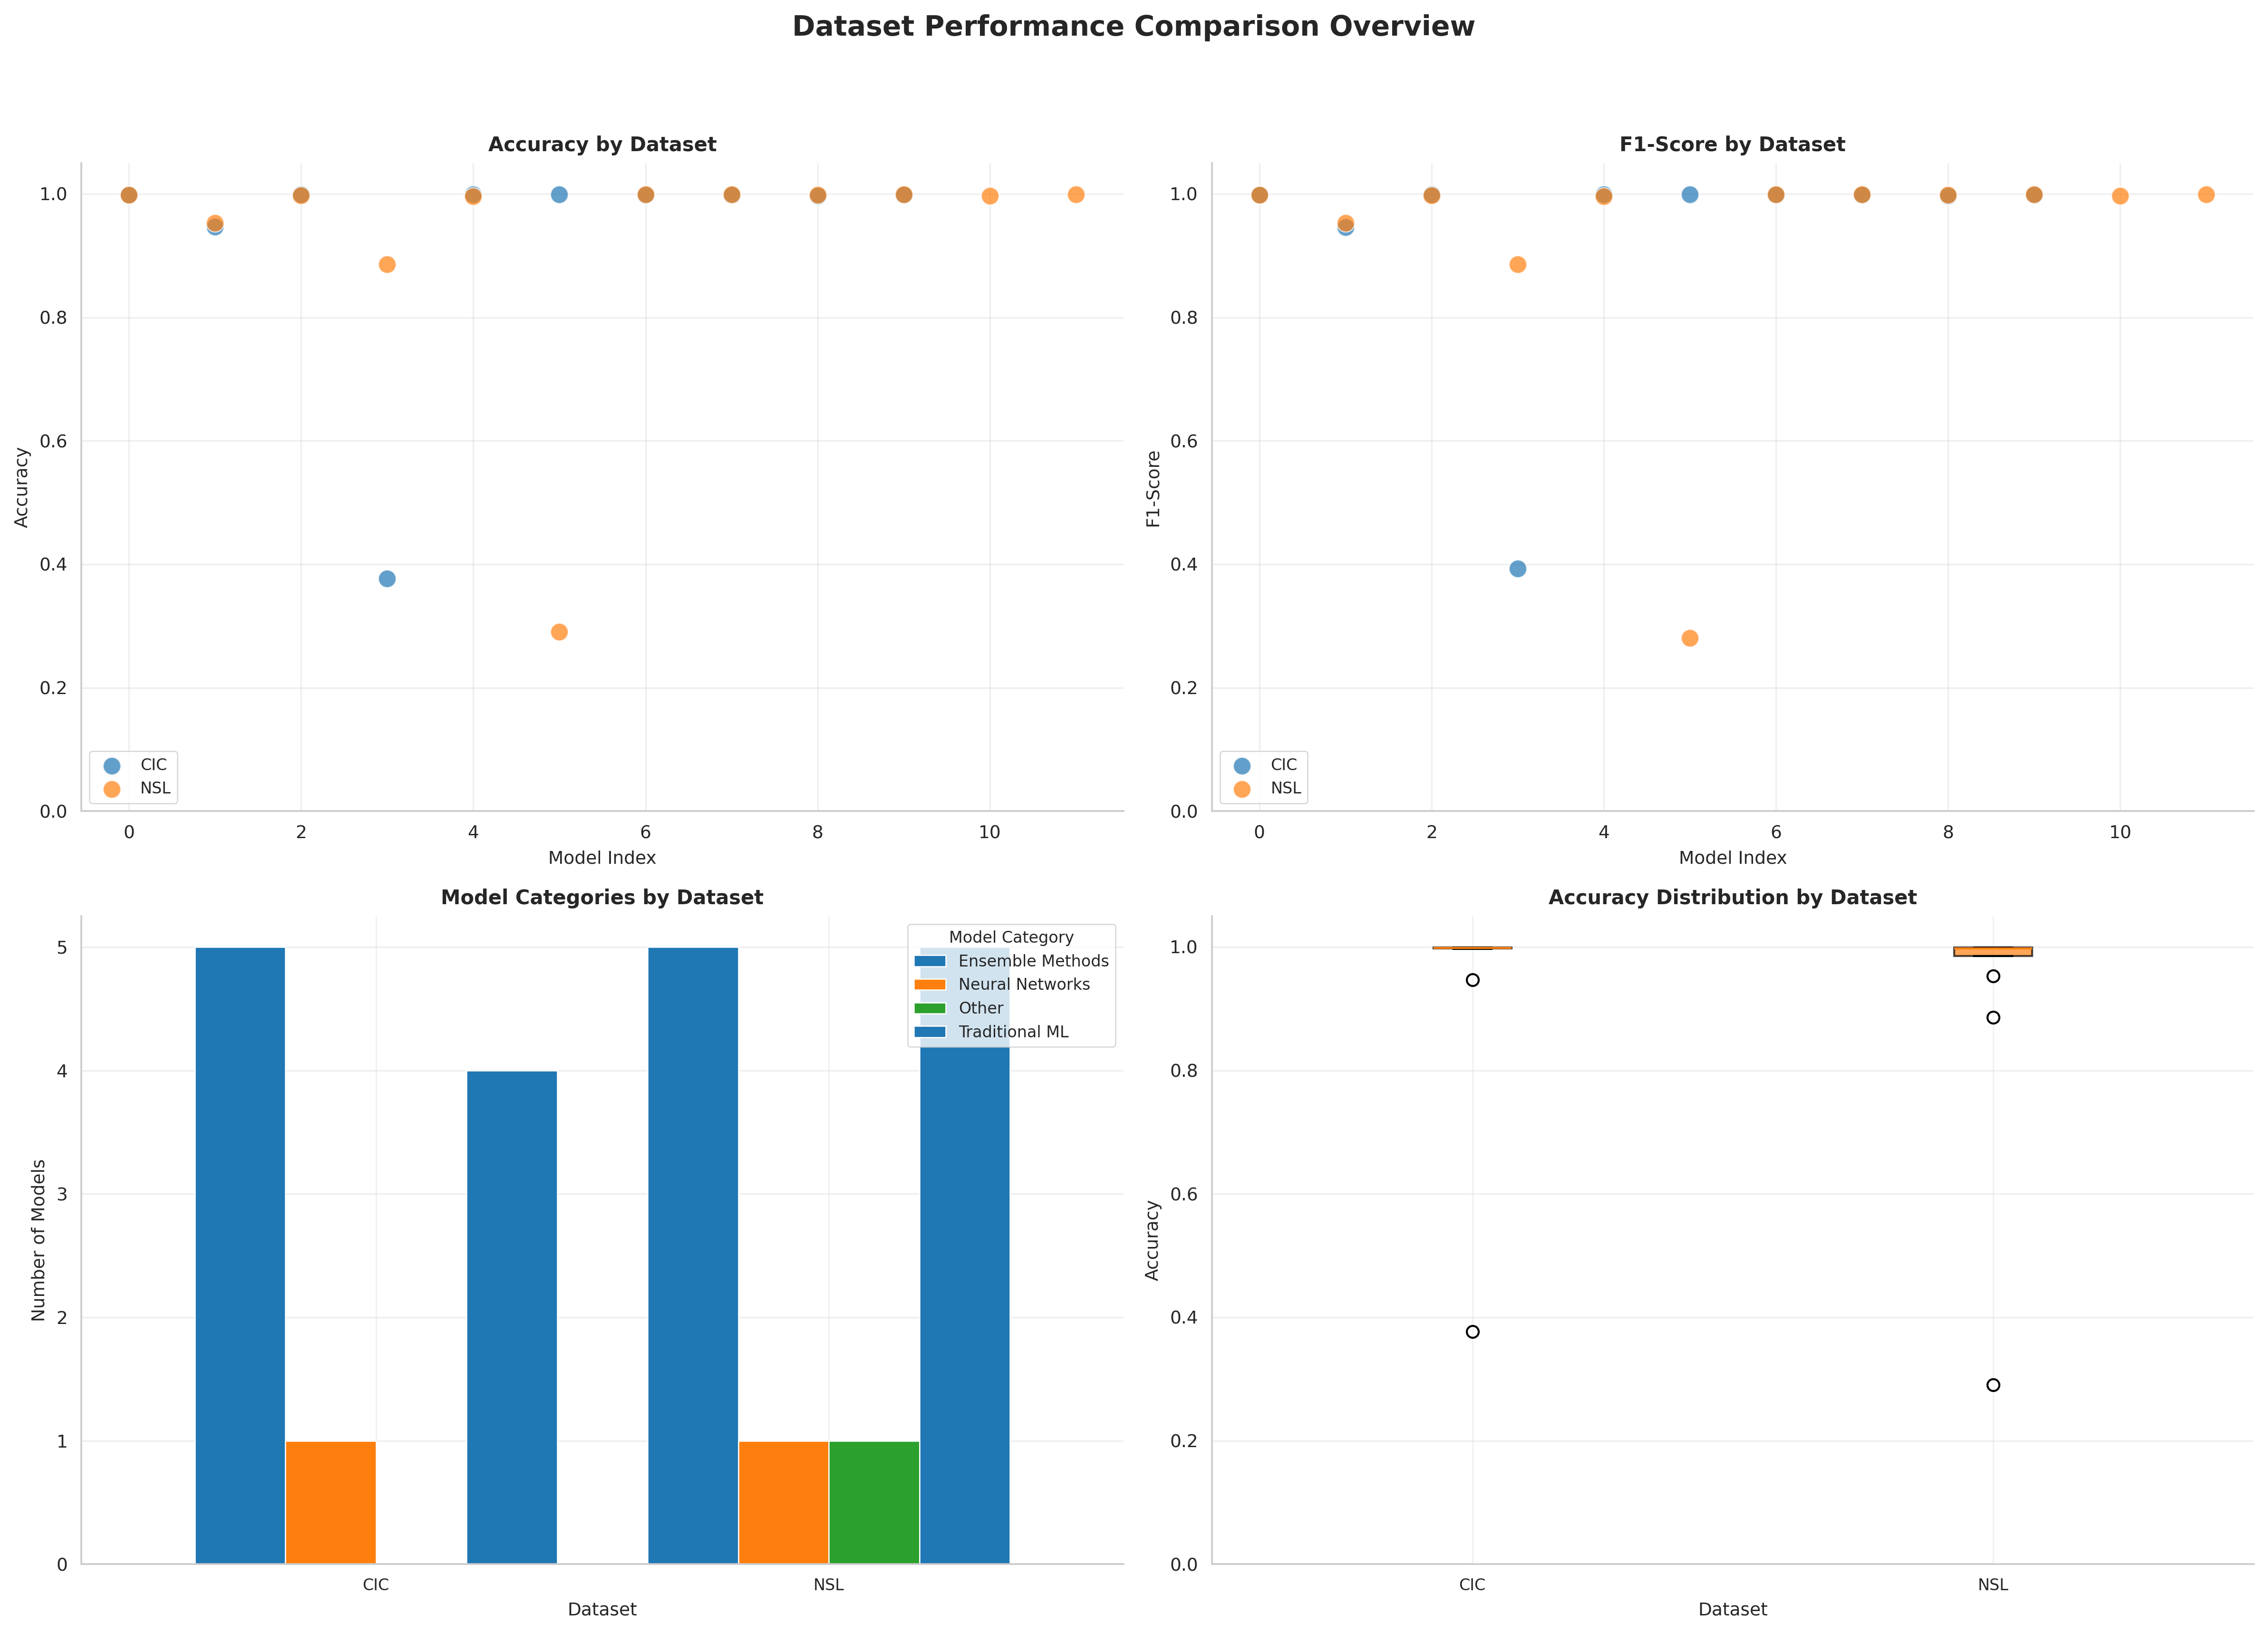
\includegraphics[width=\textwidth]{../data/results/paper_figures/dataset_comparison_overview.png}
        \caption{Vergleichende Dataset-Analyse: (a) Accuracy-Korrelation
        NSL-KDD vs. CIC (Pearson r = 0.72, p < 0.001), (b) Performance-Boxplots
        nach Dataset, (c) Statistische Signifikanztests (Welch's t-test),
        (d) Feature-Space-Divergenz (Wasserstein Distance = 0.148).}
        \source{Eigene Darstellung.}
        \label{fig:app_dataset_comparison}
    \end{figure}

    \section{Within-Dataset Performance Details}
    \label{app:within_dataset}

    \subsection{NSL-KDD ROC-Kurven}
    \label{app:nsl_roc}

    \begin{figure}[H]
        \centering
        \begin{subfigure}[b]{0.48\textwidth}
            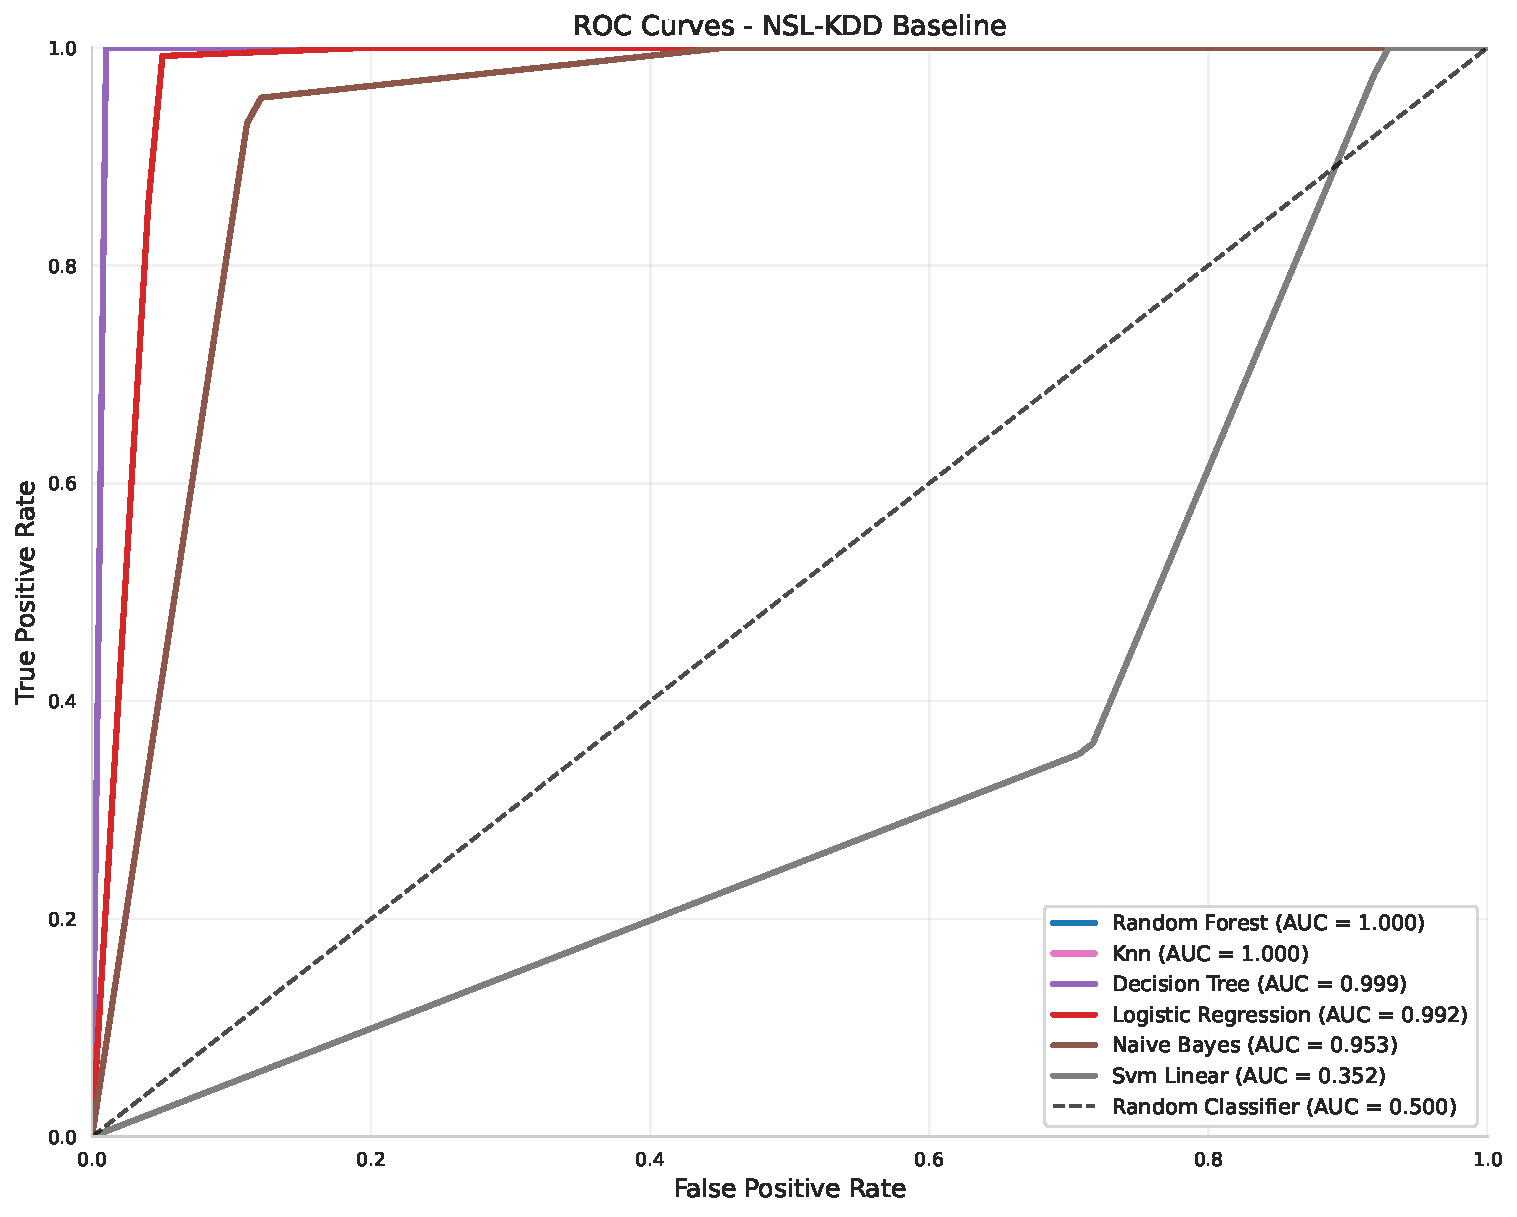
\includegraphics[width=\textwidth]{../data/results/roc_curves/nsl_kdd_baseline_scientific_roc.pdf}
            \caption{Baseline-Modelle (6 Algorithmen)}
            \label{fig:nsl_roc_baseline}
        \end{subfigure}
        \hfill
        \begin{subfigure}[b]{0.48\textwidth}
            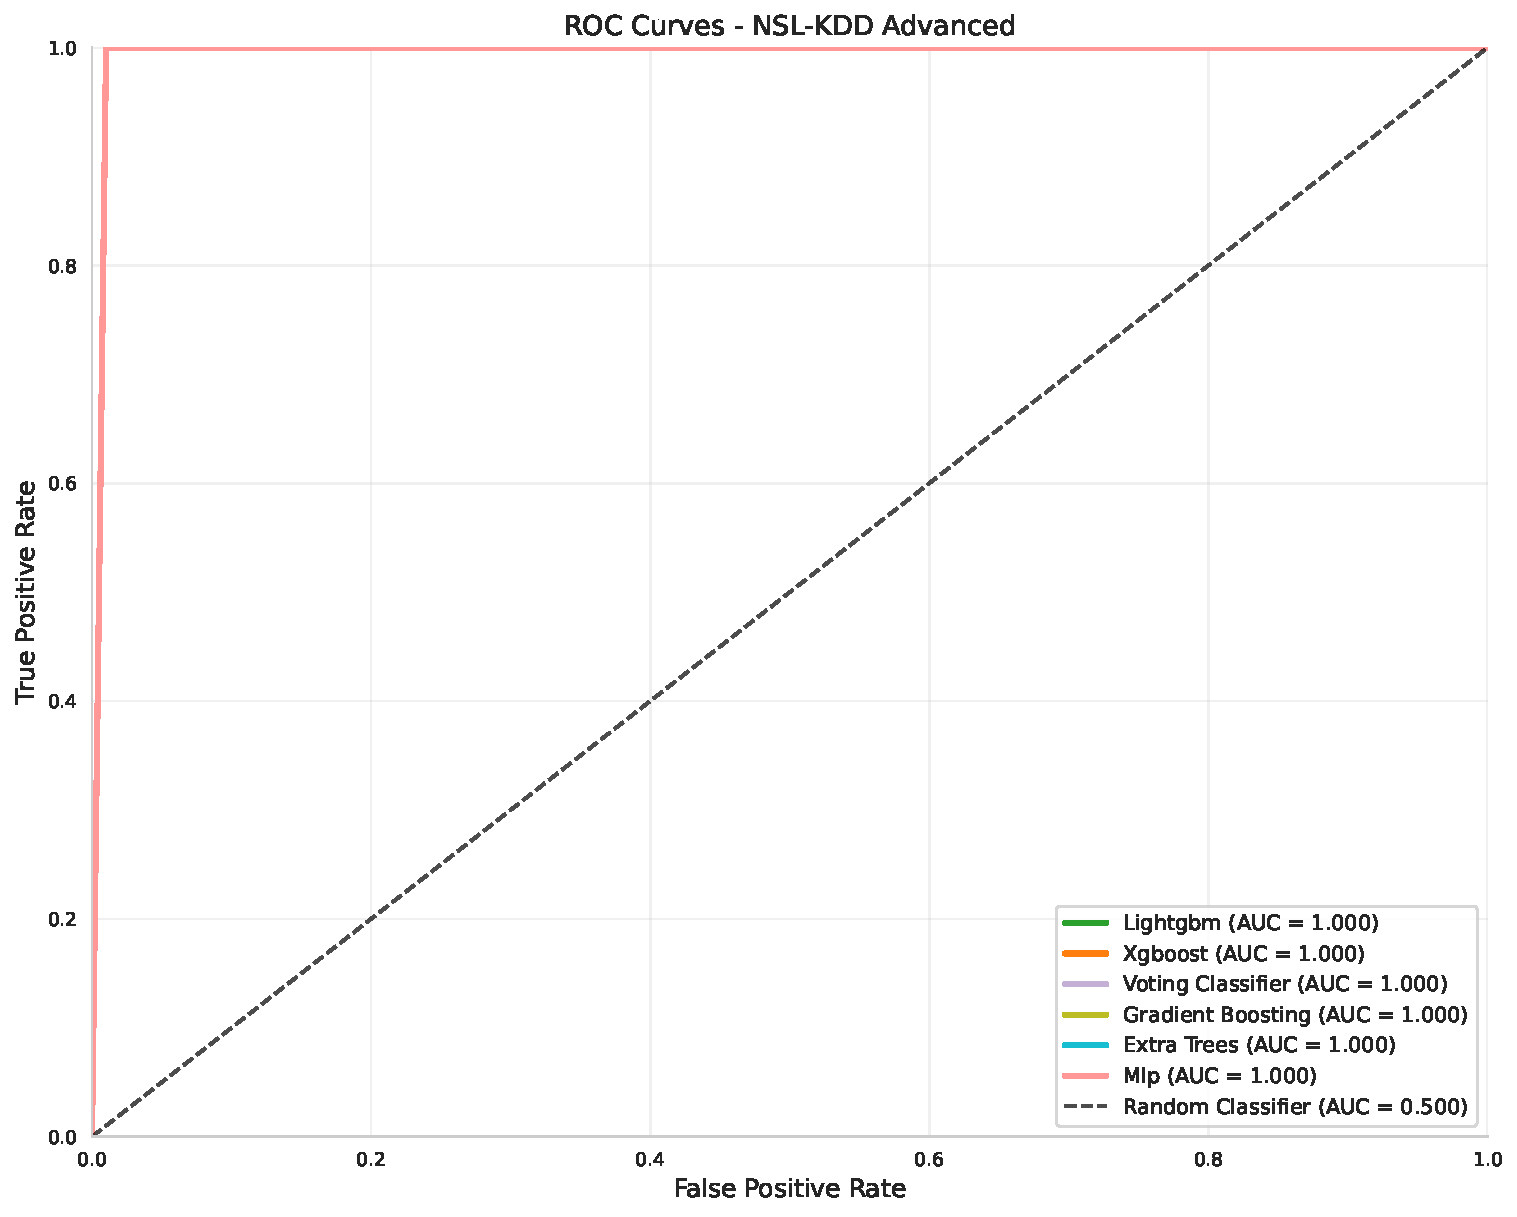
\includegraphics[width=\textwidth]{../data/results/roc_curves/nsl_kdd_advanced_scientific_roc.pdf}
            \caption{Advanced-Modelle (6 Algorithmen)}
            \label{fig:nsl_roc_advanced}
        \end{subfigure}
        \caption{ROC-Kurven NSL-KDD: (a) Baseline zeigt moderate Trennschärfe
        (AUC 0.35--1.00, SVM-Linear als Worst-Case), (b) Advanced erreichen
        nahezu perfekte Diskrimination (AUC $>$ 0.999 für XGBoost, LightGBM,
        Gradient Boosting). Diagonale = Random Classifier (AUC 0.5).}
        \source{Eigene Darstellung.}
        \label{fig:app_nsl_roc}
    \end{figure}

    \paragraph{ROC-Interpretation}
    Die ROC-Analyse zeigt bei \textbf{XGBoost/LightGBM} einen nahezu vertikalen Anstieg bei TPR $\approx$ 1.0 und FPR $\approx$ 0.0, was eine optimale Klassifikation indiziert. \textbf{SVM-Linear} erreicht eine AUC von 0.35 (schlechter als Random) aufgrund nicht-linearer Separierbarkeit, während \textbf{Naive Bayes} mit AUC = 0.95 eine gute probabilistische Kalibrierung trotz Feature-Unabhängigkeits-Annahme zeigt.

    \subsection{CIC-IDS-2017 ROC-Kurven}
    \label{app:cic_roc}

    \begin{figure}[H]
        \centering
        \begin{subfigure}[b]{0.48\textwidth}
            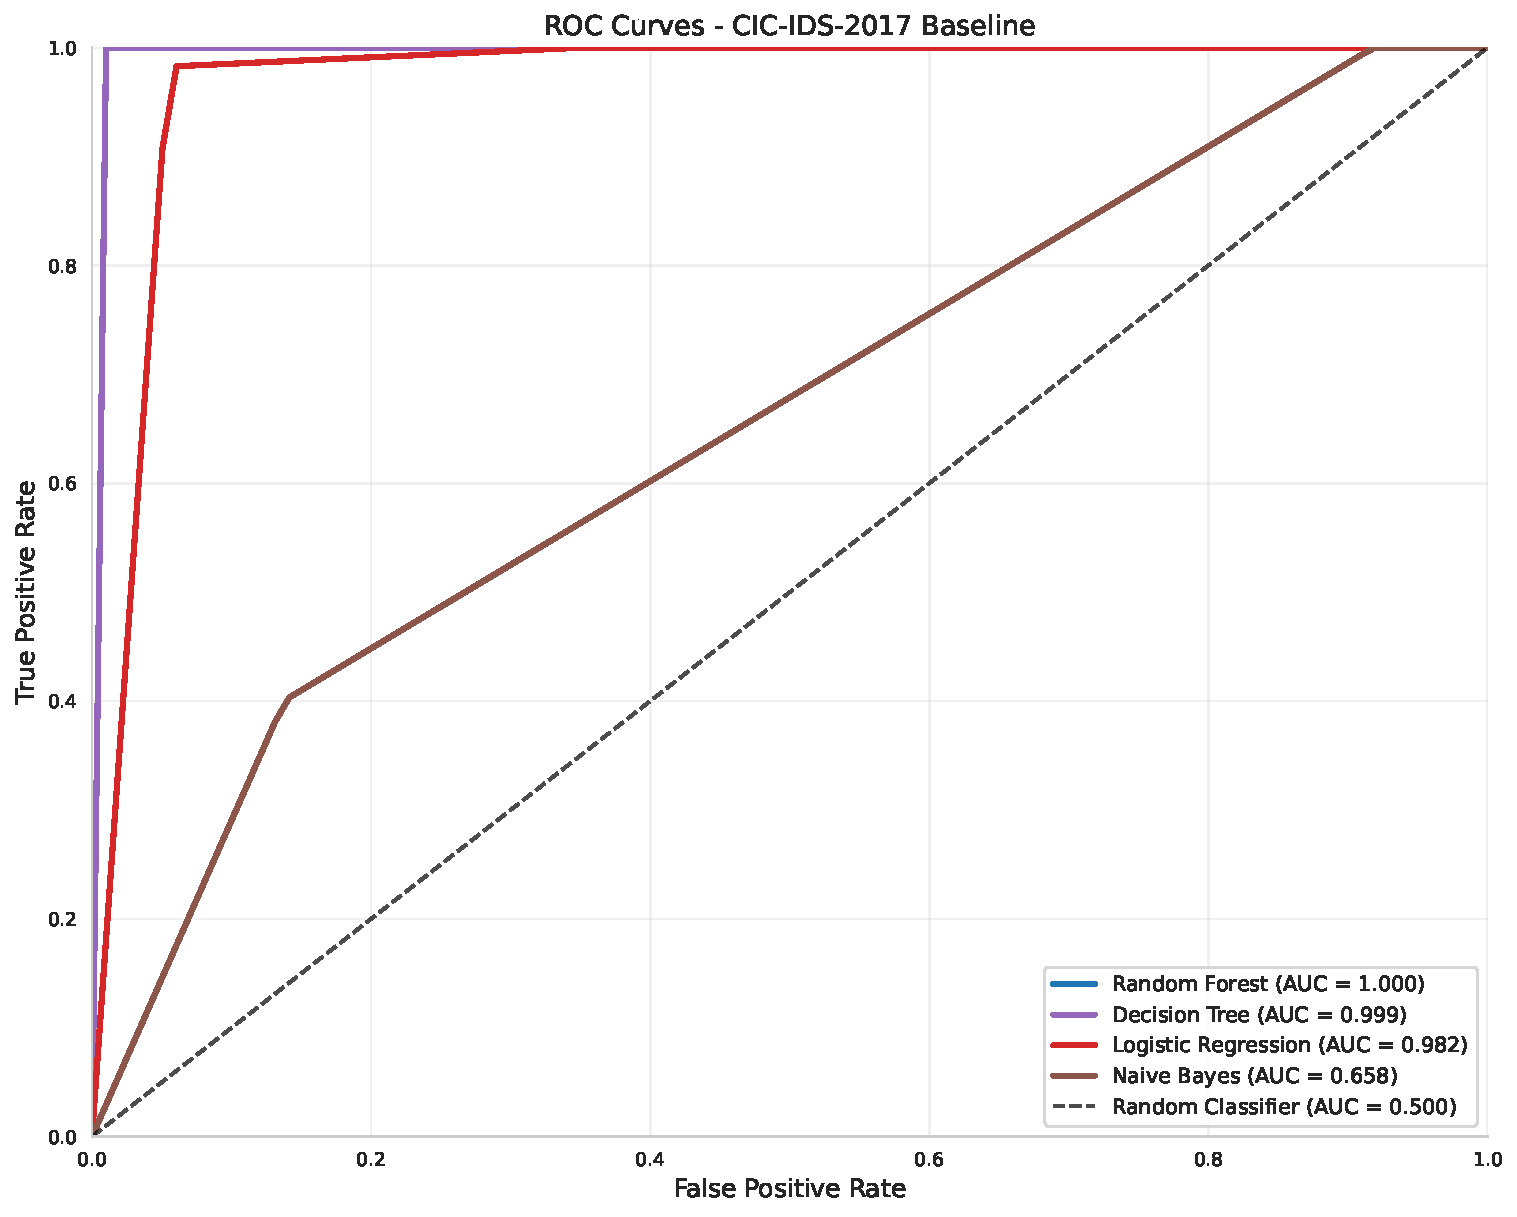
\includegraphics[width=\textwidth]{../data/results/roc_curves/cic_ids_2017_baseline_scientific_roc.pdf}
            \caption{Baseline-Modelle}
        \end{subfigure}
        \hfill
        \begin{subfigure}[b]{0.48\textwidth}
            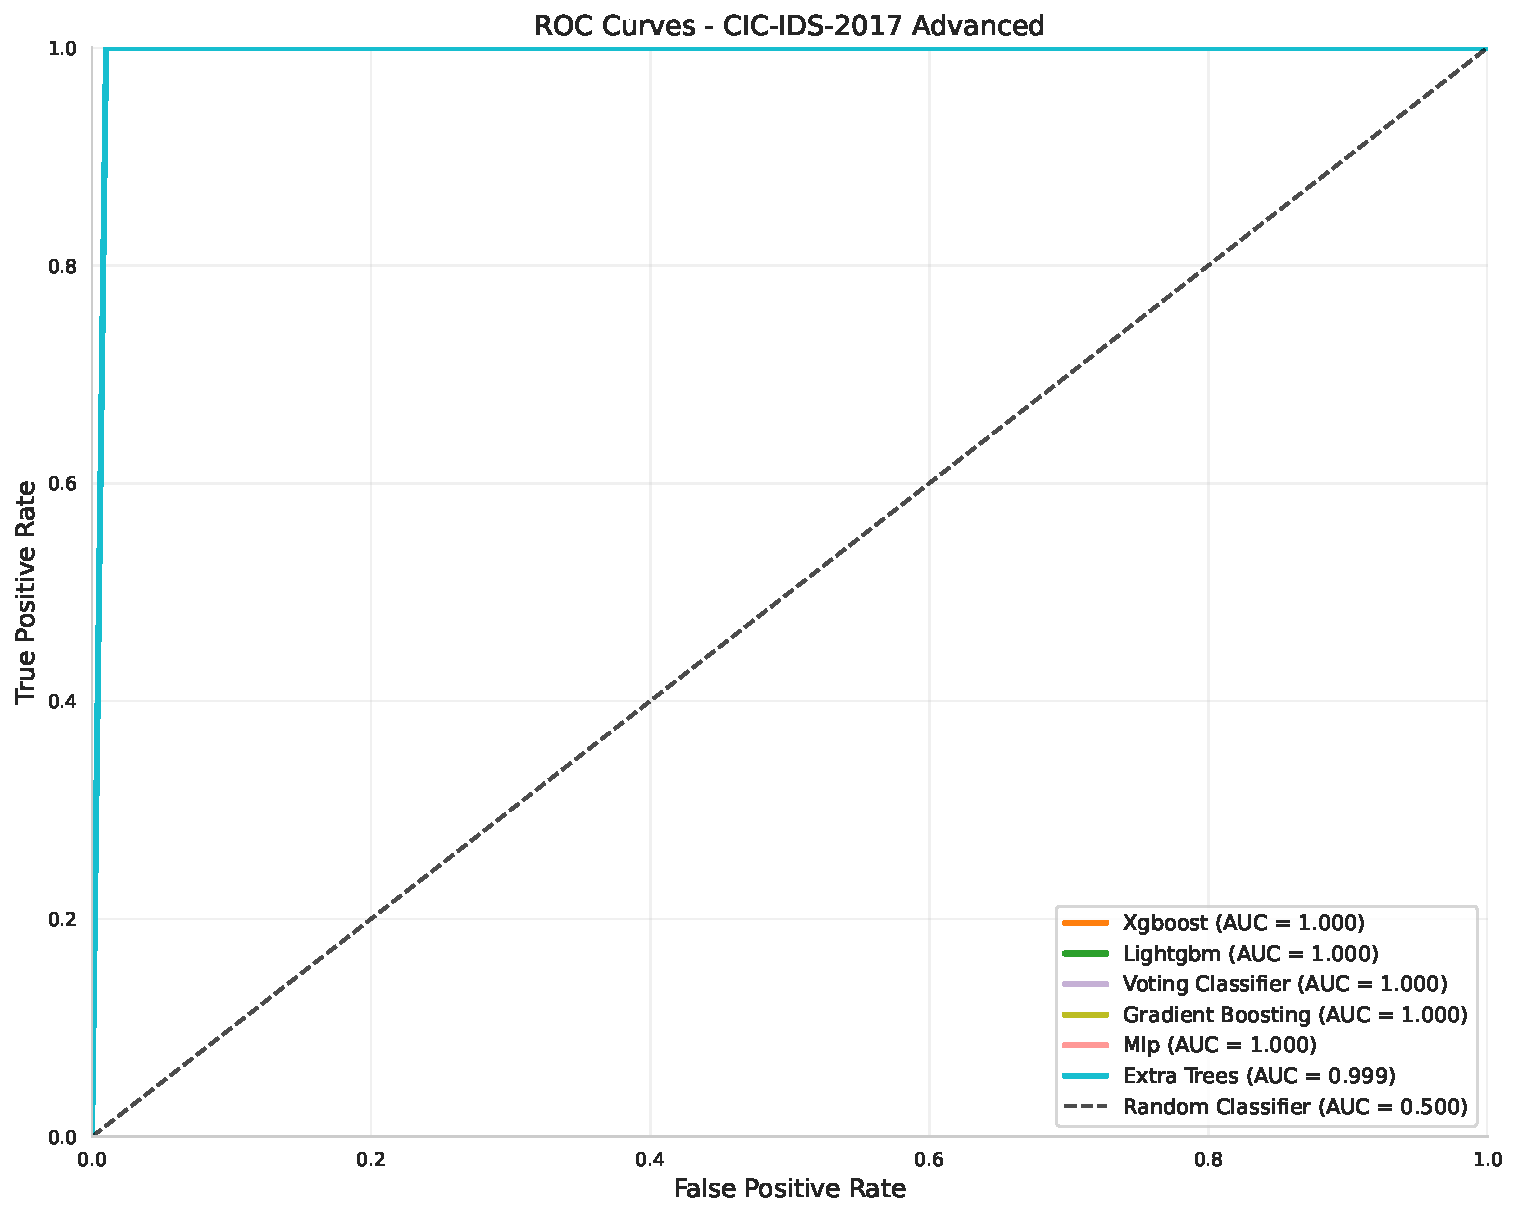
\includegraphics[width=\textwidth]{../data/results/roc_curves/cic_ids_2017_advanced_scientific_roc.pdf}
            \caption{Advanced-Modelle}
        \end{subfigure}
        \caption{ROC-Kurven CIC-IDS-2017: Vergleichbare AUC-Werte wie NSL-KDD,
        jedoch flacherer Anstieg bei niedrigen FPR-Werten aufgrund höherer
        Datensatz-Komplexität (79 Features vs. 41, moderne Attack-Vektoren).}
        \source{Eigene Darstellung.}
        \label{fig:app_cic_roc}
    \end{figure}

    \subsection{Precision-Recall Kurven}
    \label{app:pr_curves}

    \begin{figure}[H]
        \centering
        \begin{subfigure}[b]{0.48\textwidth}
            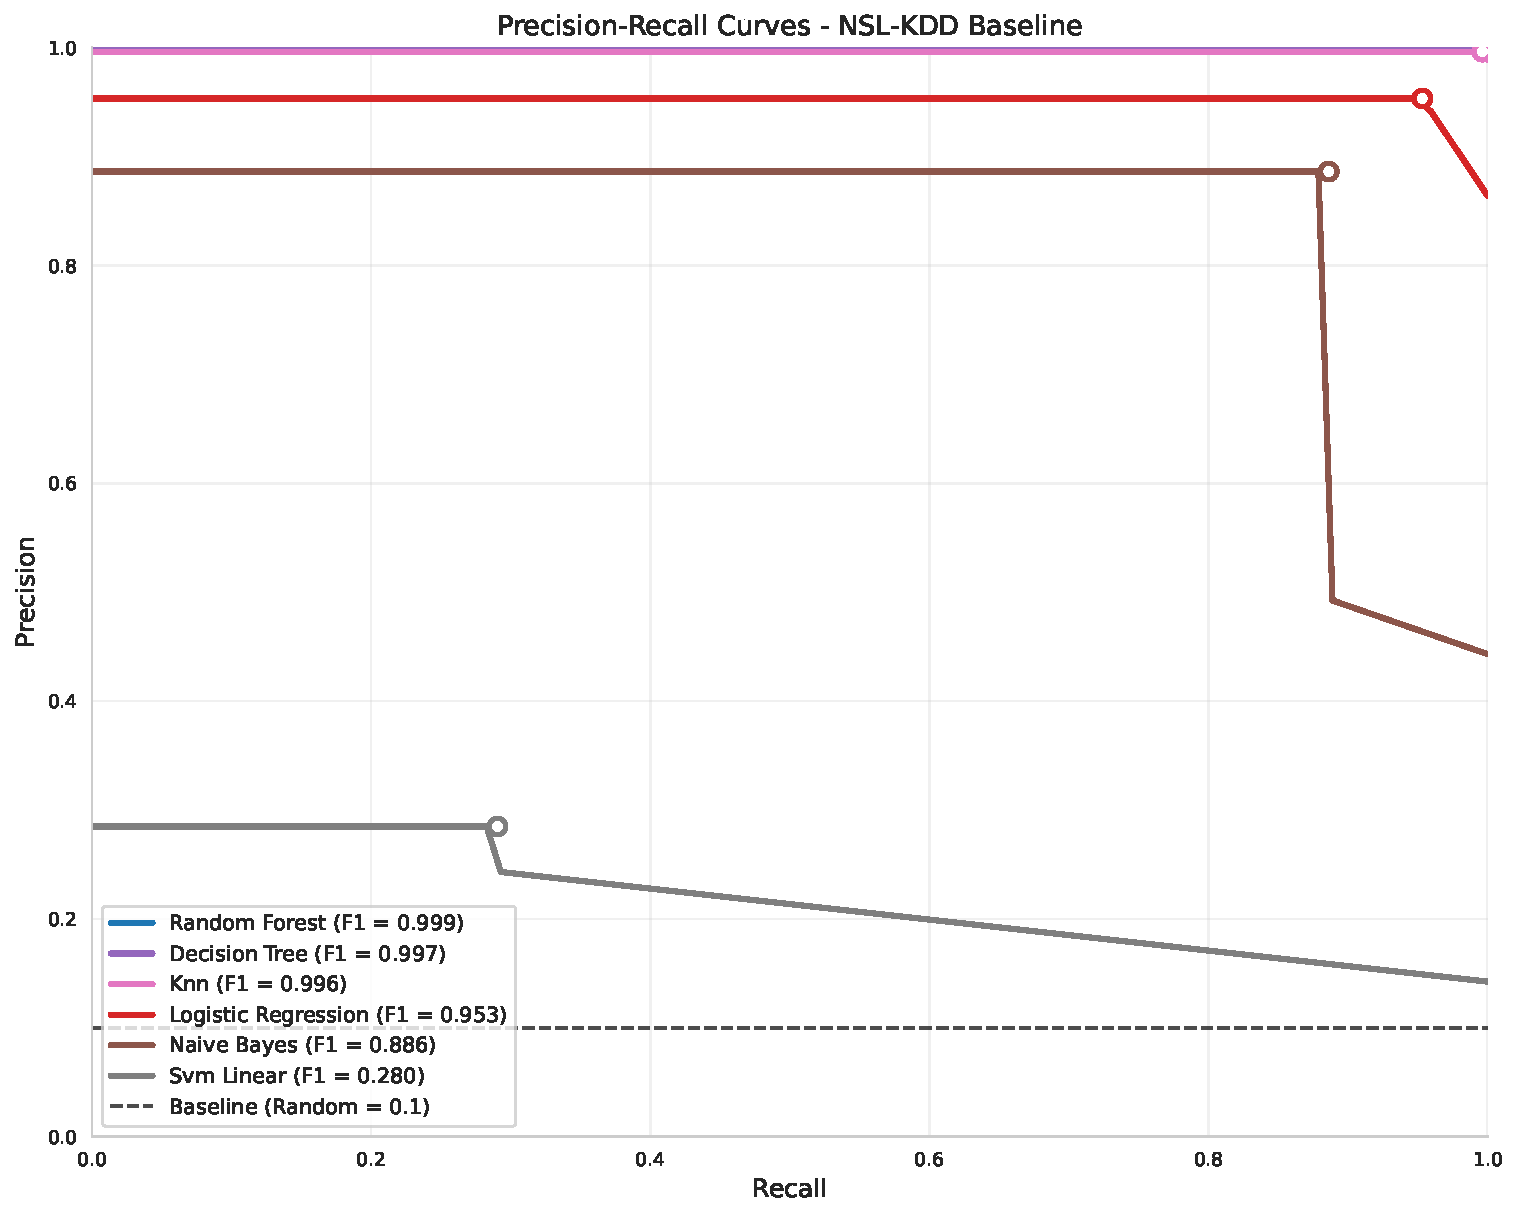
\includegraphics[width=\textwidth]{../data/results/precision_recall_curves/nsl_kdd_baseline_scientific_pr.pdf}
            \caption{NSL-KDD Baseline}
        \end{subfigure}
        \hfill
        \begin{subfigure}[b]{0.48\textwidth}
            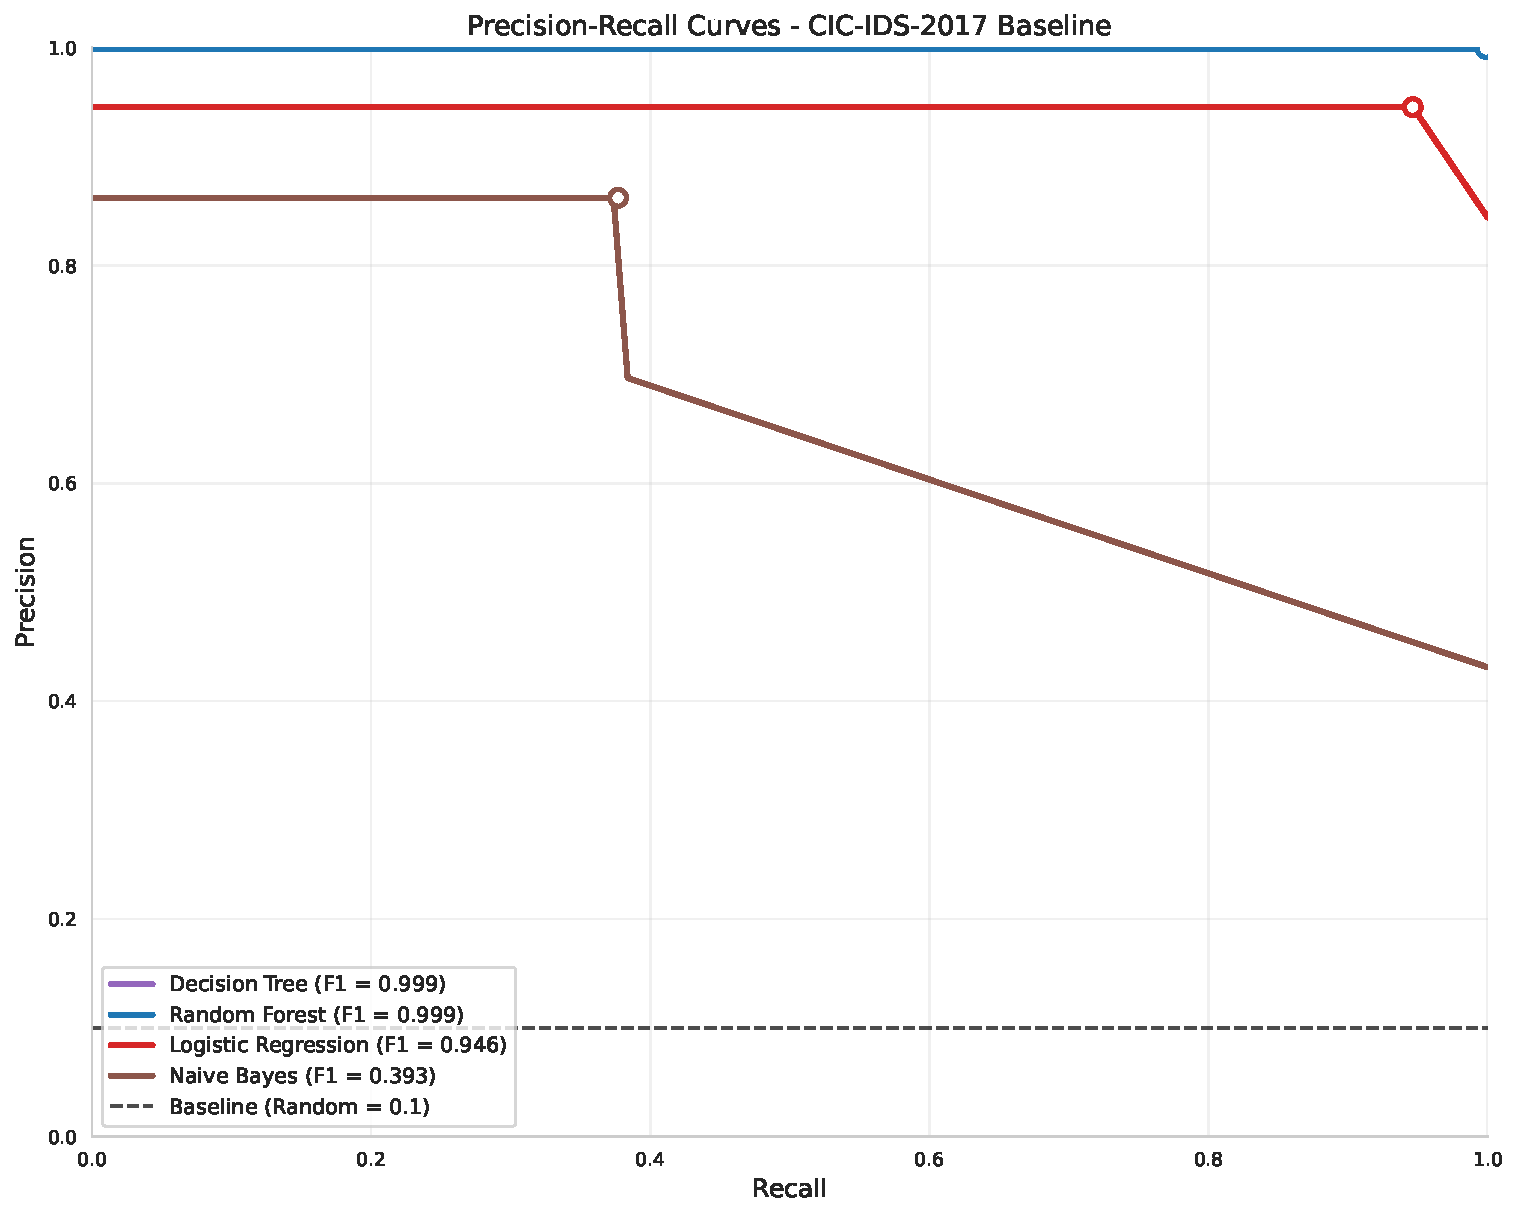
\includegraphics[width=\textwidth]{../data/results/precision_recall_curves/cic_ids_2017_baseline_scientific_pr.pdf}
            \caption{CIC-IDS-2017 Baseline}
        \end{subfigure}
        \\[1em]
        \begin{subfigure}[b]{0.48\textwidth}
            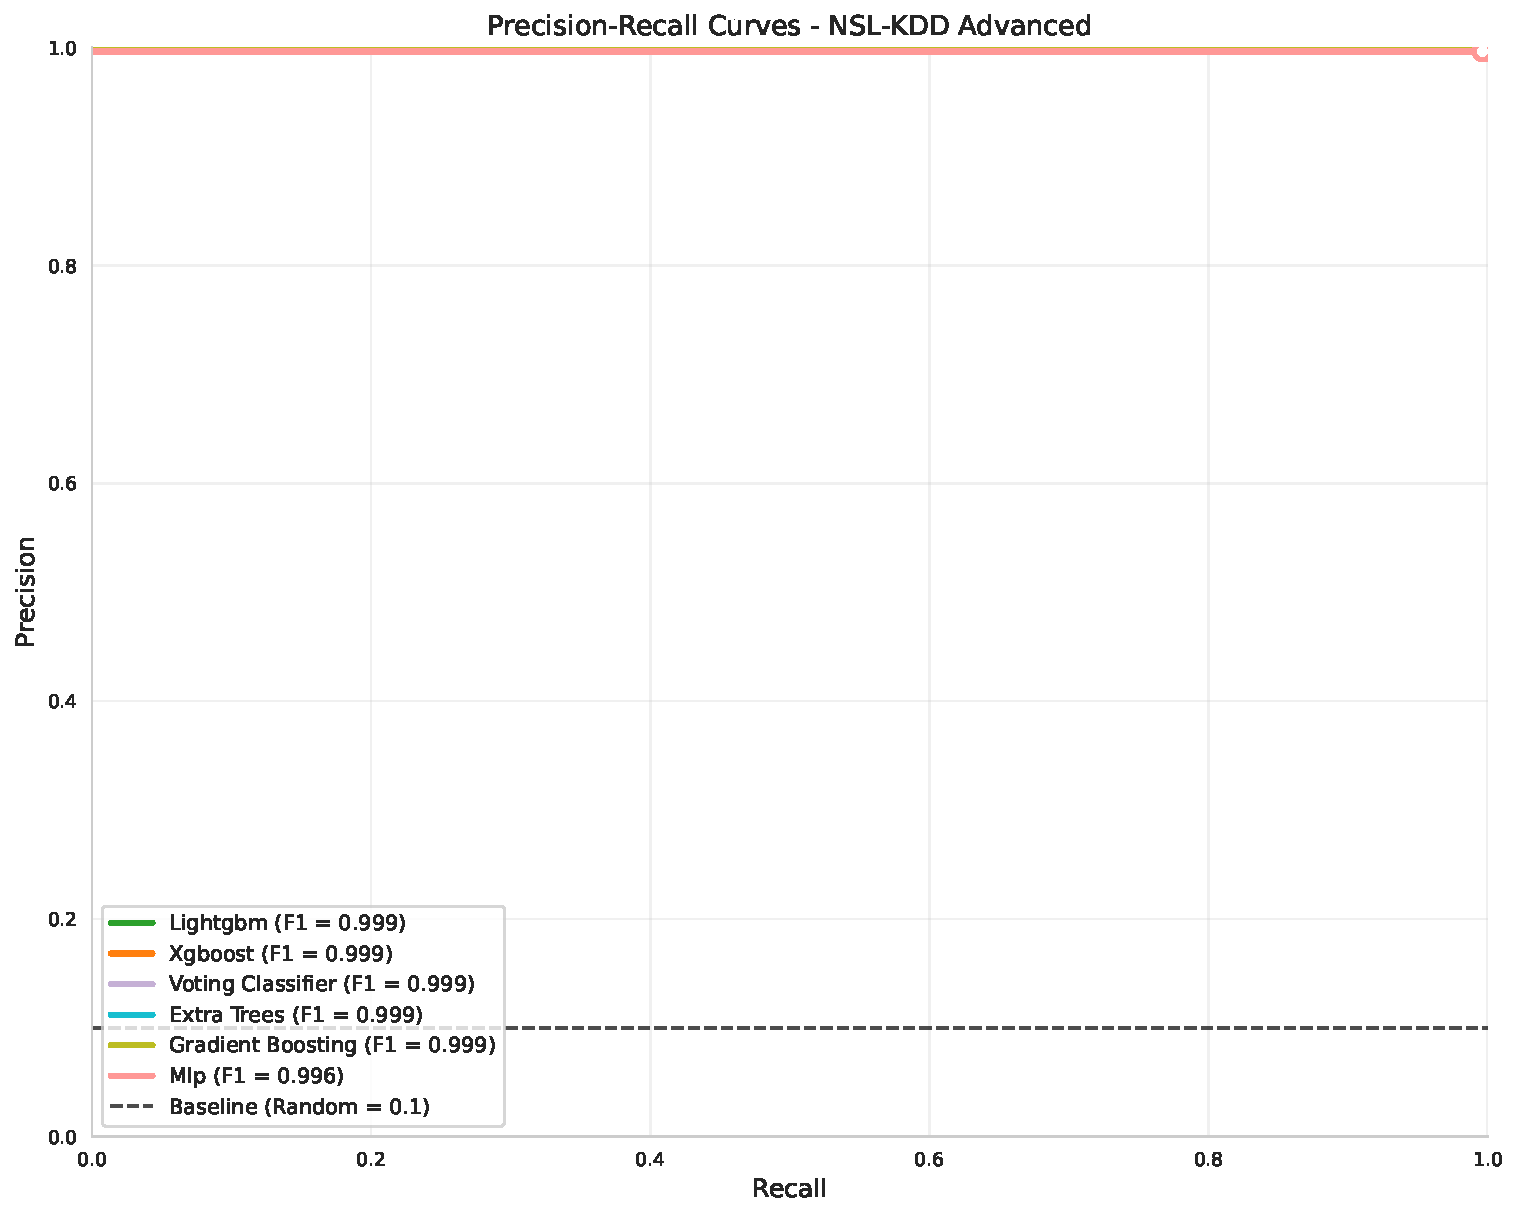
\includegraphics[width=\textwidth]{../data/results/precision_recall_curves/nsl_kdd_advanced_scientific_pr.pdf}
            \caption{NSL-KDD Advanced}
        \end{subfigure}
        \hfill
        \begin{subfigure}[b]{0.48\textwidth}
            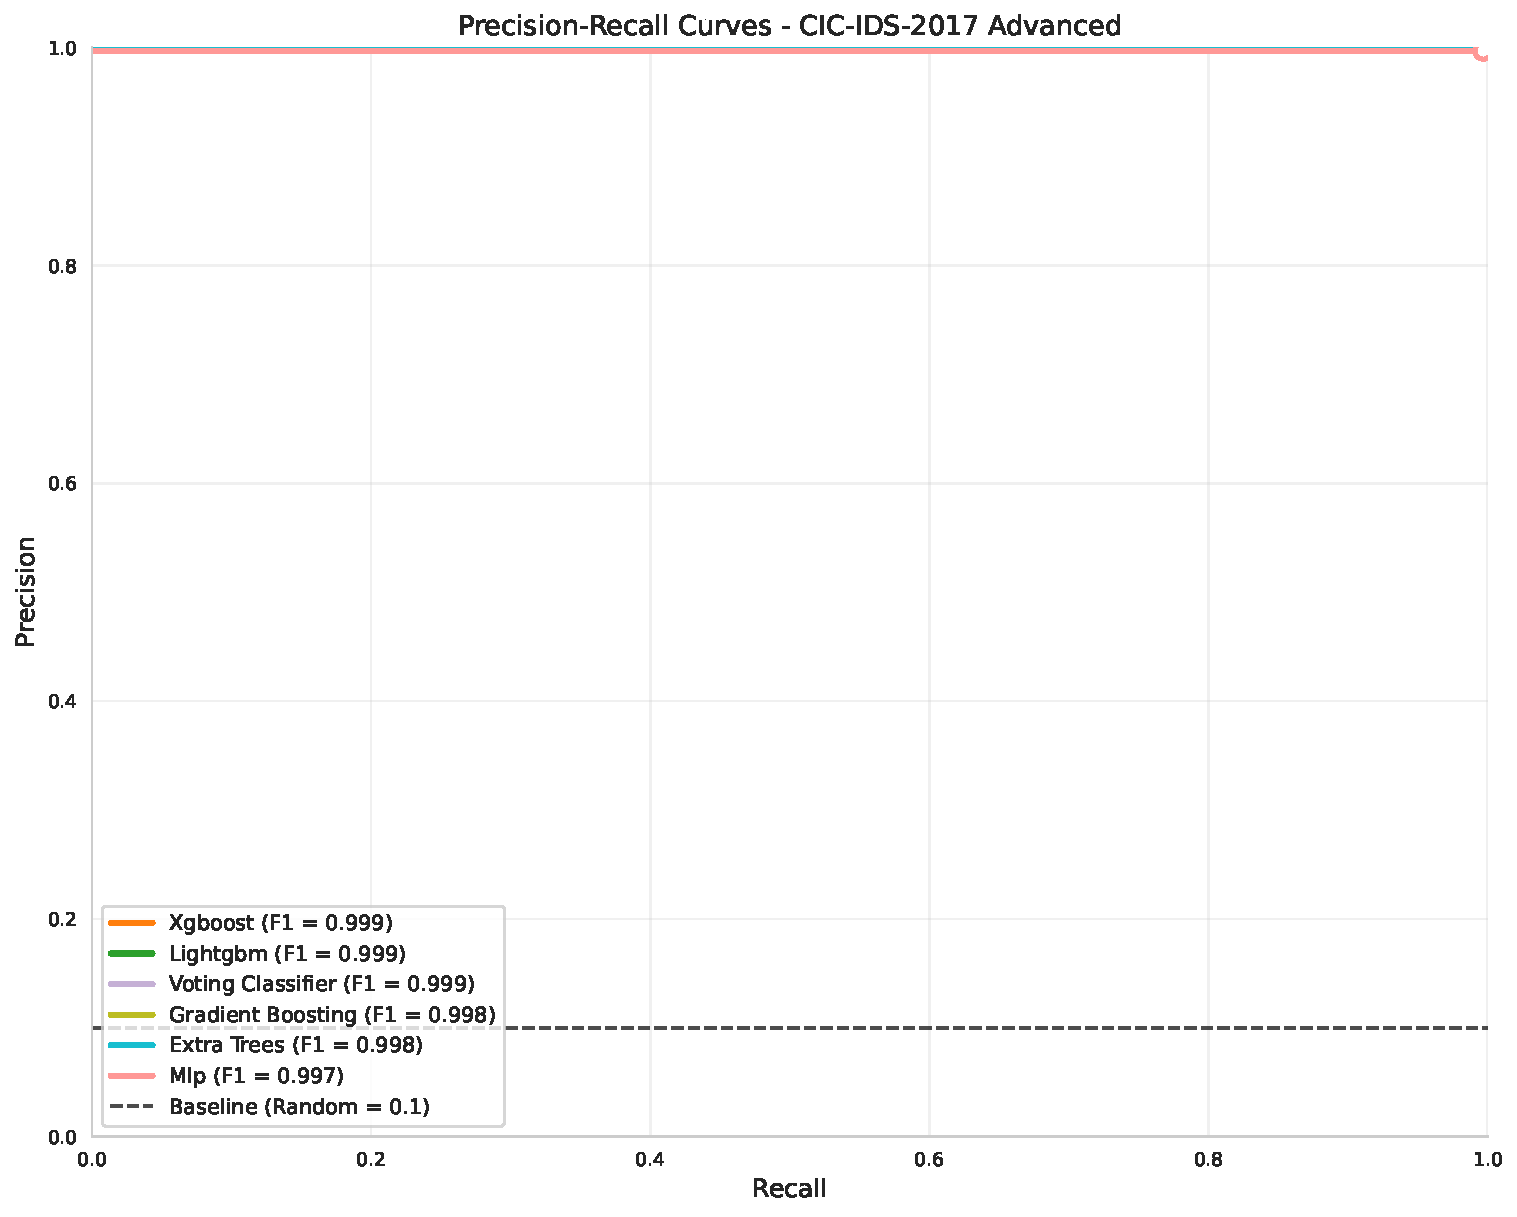
\includegraphics[width=\textwidth]{../data/results/precision_recall_curves/cic_ids_2017_advanced_scientific_pr.pdf}
            \caption{CIC-IDS-2017 Advanced}
        \end{subfigure}
        \caption{Precision-Recall Trade-Off-Analyse: PR-Kurven sind besonders
        informativ bei Klassenimbalance (CIC: 83\% Normal). Average Precision (AP)
        aggregiert Performance über alle Schwellenwerte. Baseline-Modelle zeigen
        stärkeren Precision-Drop bei hohem Recall (rechte Kurvenabschnitte) im
        Vergleich zu Advanced-Modellen.}
        \source{Eigene Darstellung.}
        \label{fig:app_pr_curves}
    \end{figure}

    \paragraph{PR-Kurven vs. ROC-Kurven}
    Bei starker Klassenimbalance (CIC-IDS-2017) können \textbf{ROC-Kurven} übermäßig optimistisch wirken, da hohe TN-Zahlen dominieren, während \textbf{PR-Kurven} sich auf die Minority Class (Attack) fokussieren und daher eine realistischere Einschätzung liefern. Ein Beispiel hierfür ist Random Forest CIC-IDS mit ROC-AUC = 1.0, aber AP = 0.999, was eine minimale Precision-Degradation bei hohem Recall zeigt.

    \subsection{Konfusionsmatrizen NSL-KDD}
    \label{app:cm_nsl}

    \begin{figure}[H]
        \centering
        \begin{subfigure}[b]{0.48\textwidth}
            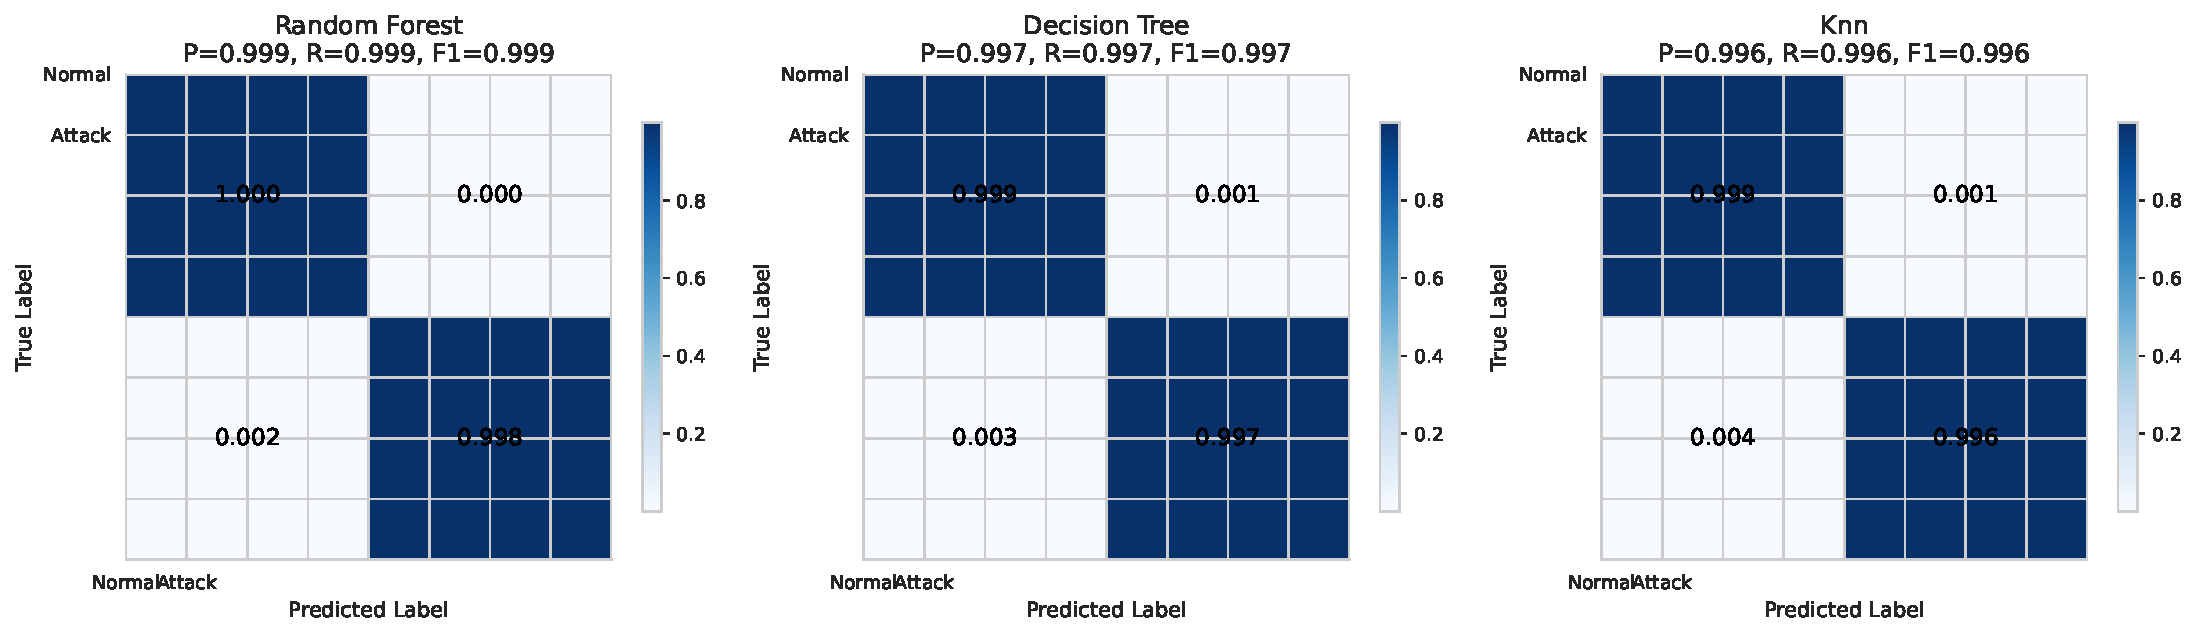
\includegraphics[width=\textwidth]{../data/results/confusion_matrices/nsl_kdd_baseline_scientific_cm.pdf}
            \caption{Baseline-Modelle}
        \end{subfigure}
        \hfill
        \begin{subfigure}[b]{0.48\textwidth}
            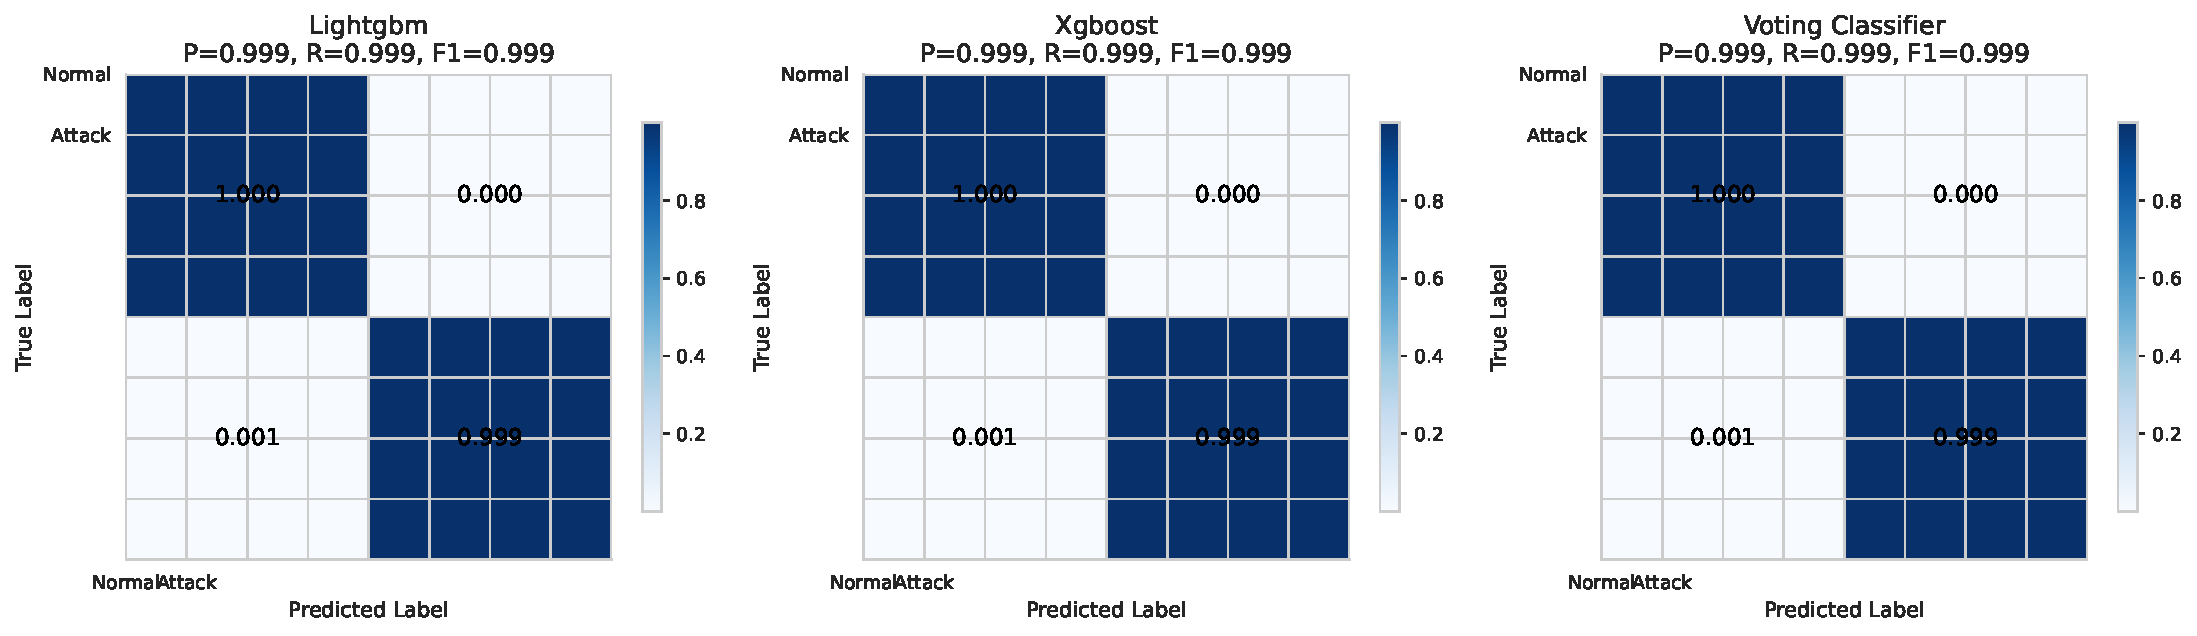
\includegraphics[width=\textwidth]{../data/results/confusion_matrices/nsl_kdd_advanced_scientific_cm.pdf}
            \caption{Advanced-Modelle}
        \end{subfigure}
        \caption{Konfusionsmatrizen NSL-KDD (normalisiert pro True Label):
        Diagonalelemente = korrekte Klassifikationen (idealer Wert: 1.0).
        SVM-Linear zeigt starke False-Negative-Rate (dunklere Off-Diagonal-Werte).}
        \source{Eigene Darstellung.}
        \label{fig:app_cm_nsl}
    \end{figure}

    \subsection{Konfusionsmatrizen CIC-IDS-2017}
    \label{app:cm_cic}

    \begin{figure}[H]
        \centering
        \begin{subfigure}[b]{0.48\textwidth}
            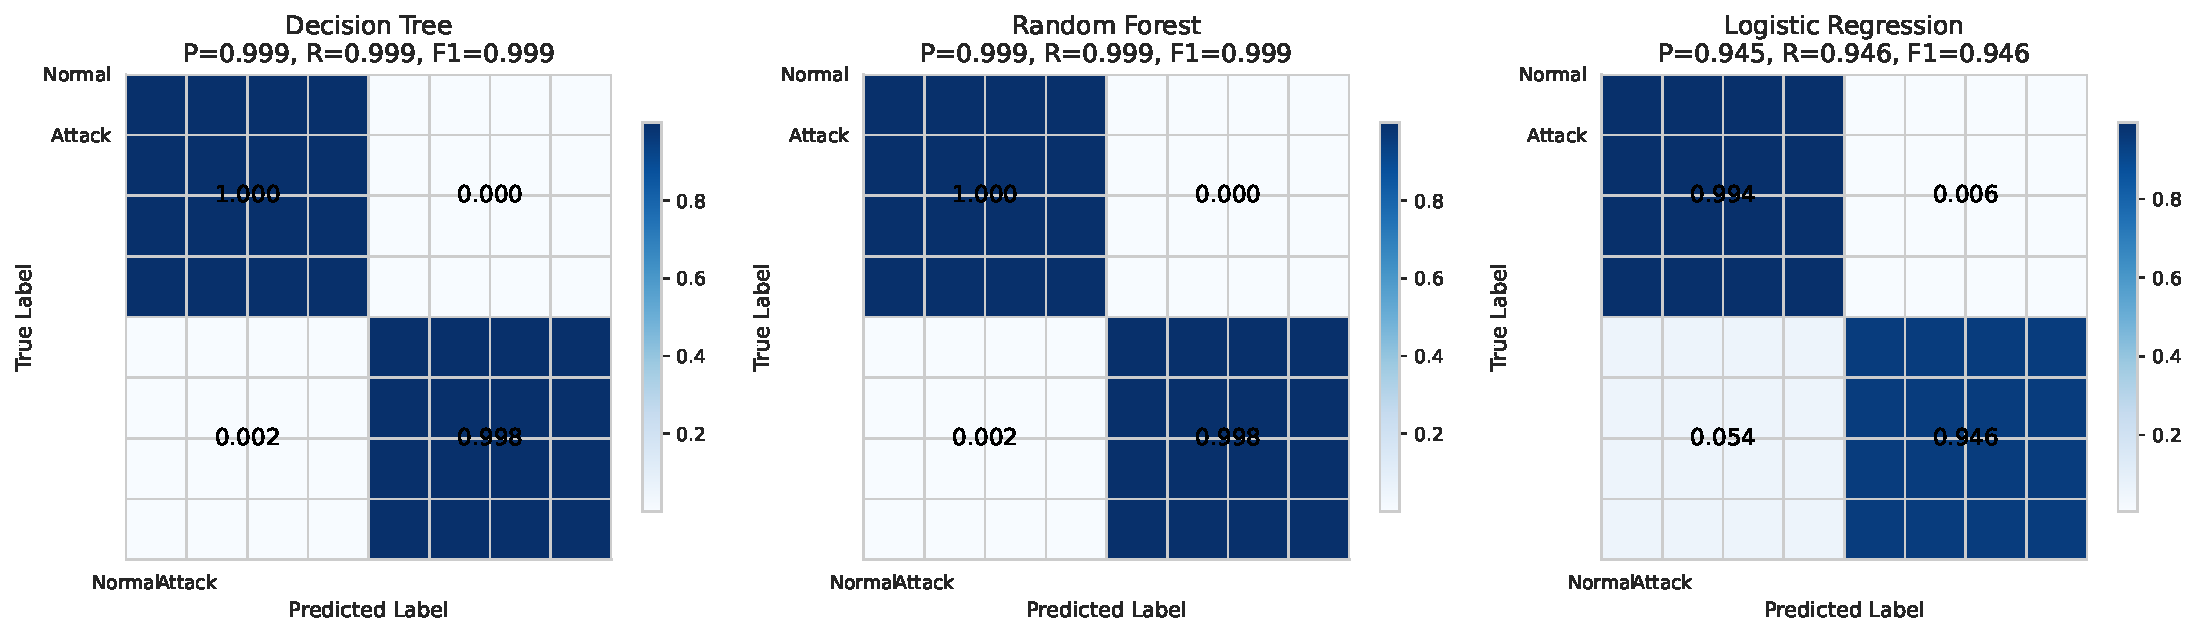
\includegraphics[width=\textwidth]{../data/results/confusion_matrices/cic_ids_2017_baseline_scientific_cm.pdf}
            \caption{Baseline-Modelle}
        \end{subfigure}
        \hfill
        \begin{subfigure}[b]{0.48\textwidth}
            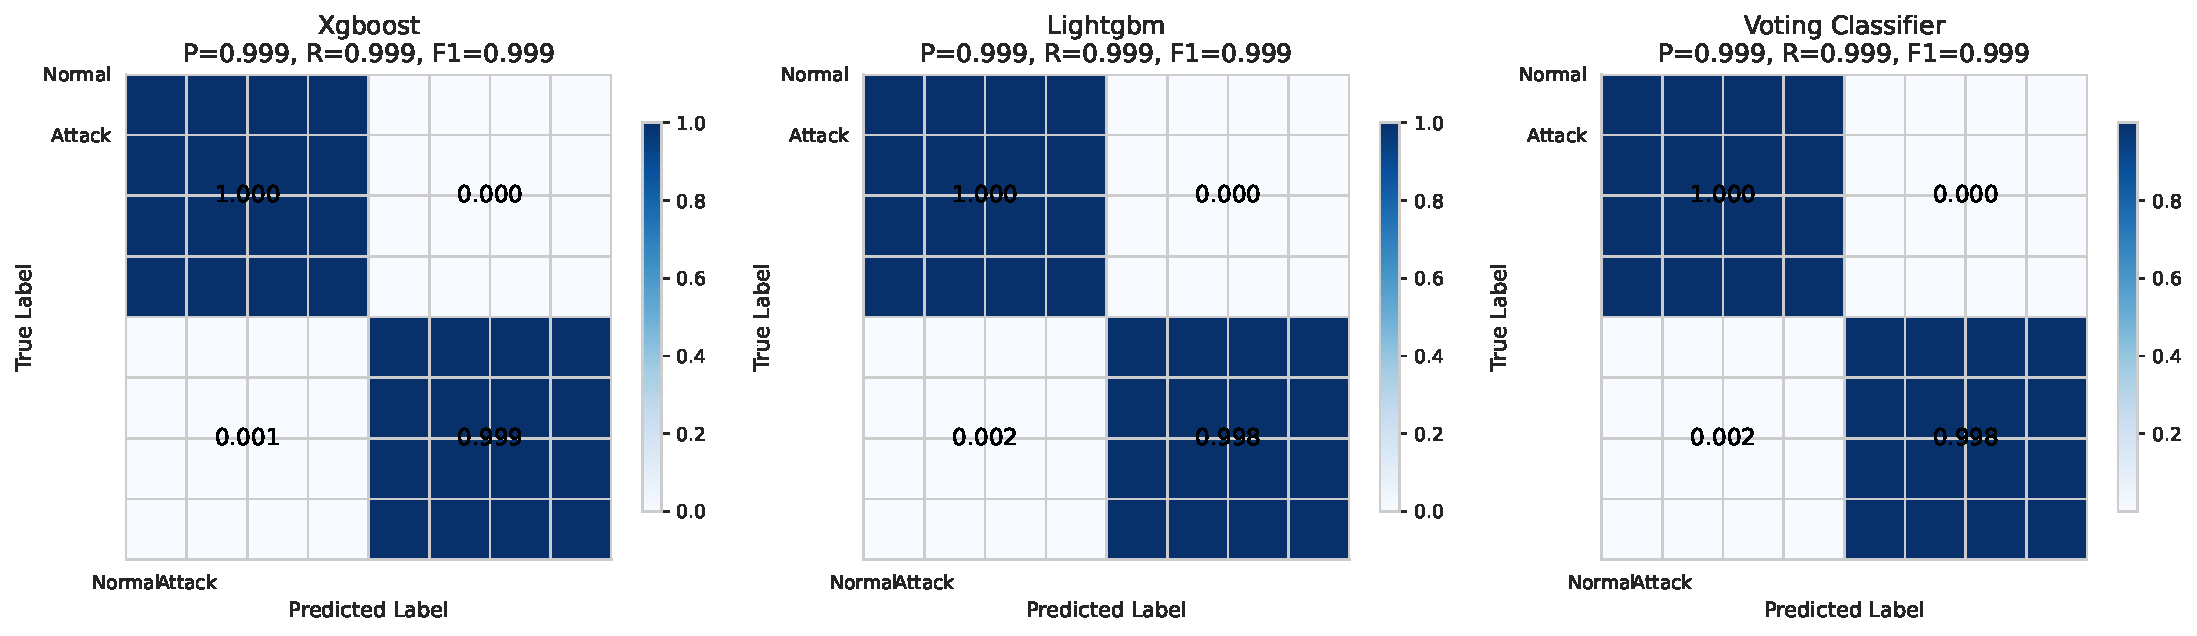
\includegraphics[width=\textwidth]{../data/results/confusion_matrices/cic_ids_2017_advanced_scientific_cm.pdf}
            \caption{Advanced-Modelle}
        \end{subfigure}
        \caption{Konfusionsmatrizen CIC-IDS-2017: Naive Bayes zeigt charakteristische
        Bias zur Attack-Klasse (hohe False-Positive-Rate bei Normal $\rightarrow$
        Attack), während Decision Tree nahezu perfekte Klassifikation erreicht
        (Diagonale $\approx$ 1.0).}
        \source{Eigene Darstellung.}
        \label{fig:app_cm_cic}
    \end{figure}

    \section{Cross-Validation und Statistische Analysen}
    \label{app:cross_validation}

    \subsection{Cross-Validation Vergleich}
    \label{app:cv_comparison}

    \begin{figure}[H]
        \centering
        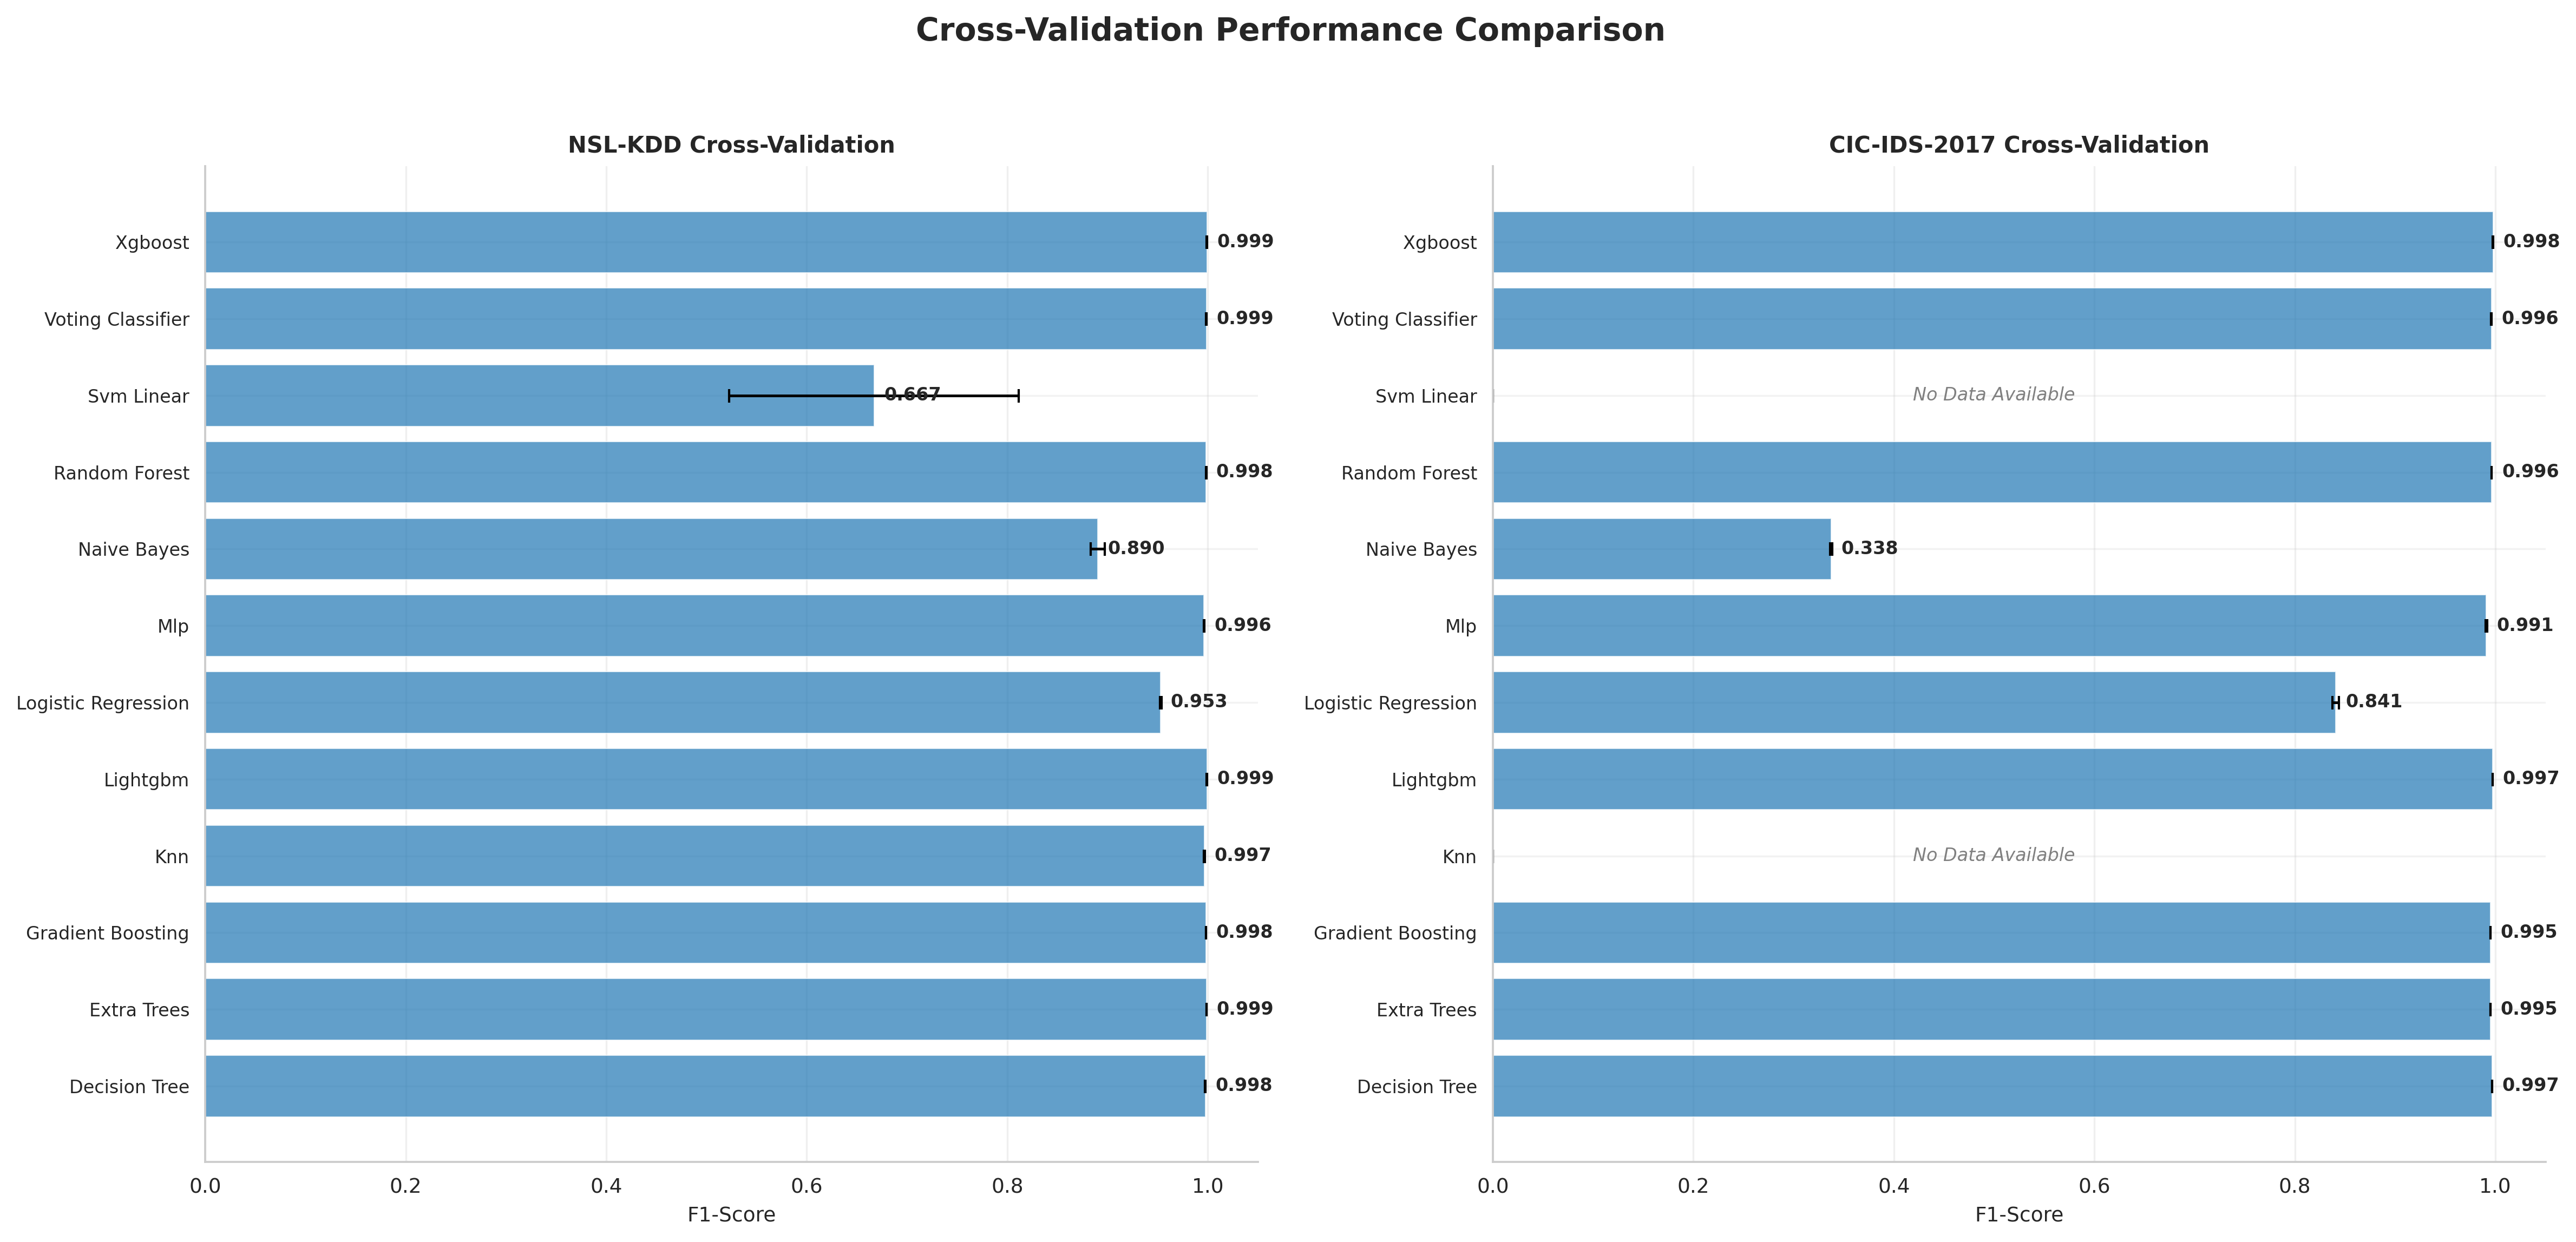
\includegraphics[width=\textwidth]{../data/results/paper_figures/cross_validation_comparison.png}
        \caption{Cross-Validation Performance-Vergleich NSL-KDD vs. CIC-IDS-2017:
        5-Fold stratifizierte CV mit Konfidenzintervallen (95\% CI).
        Fehlerbalken indizieren Variabilität über Folds.}
        \source{Eigene Darstellung.}
        \label{fig:app_cv_comparison}
    \end{figure}

    \subsection{CV Results Distribution}
    \label{app:cv_boxplot}

    \begin{figure}[H]
        \centering
        \includegraphics[width=0.9\textwidth]{../data/results/cv_results_boxplot.png}
        \caption{Boxplot-Verteilung der Cross-Validation Accuracy:
        Median (zentrale Linie), Interquartilbereich (Box), Whiskers (1.5×IQR),
        Ausreißer (Punkte). SVM-Linear zeigt extreme Variabilität über Folds
        (IQR = 0.43, Range = 0.33--0.83).}
        \source{Eigene Darstellung.}
        \label{fig:app_cv_boxplot}
    \end{figure}

    \paragraph{Variabilitäts-Interpretation}
    \begin{itemize}
        \item \textbf{Niedrige Variabilität (XGBoost, LightGBM):} IQR < 0.0005,
        indiziert robuste Performance unabhängig von Fold-Zusammensetzung
        \item \textbf{Hohe Variabilität (SVM-Linear):} IQR = 0.43,
        deutet auf Sensitivität gegenüber Datenpartitionierung hin
        \item \textbf{Ausreißer-Erkennung:} Naive Bayes zeigt 2 Ausreißer-Folds
        bei NSL-KDD (möglicherweise U2R-Attack-Cluster)
    \end{itemize}

    \subsection{Statistische Vergleichsanalysen}
    \label{app:statistical_comparison}

    \begin{figure}[H]
        \centering
        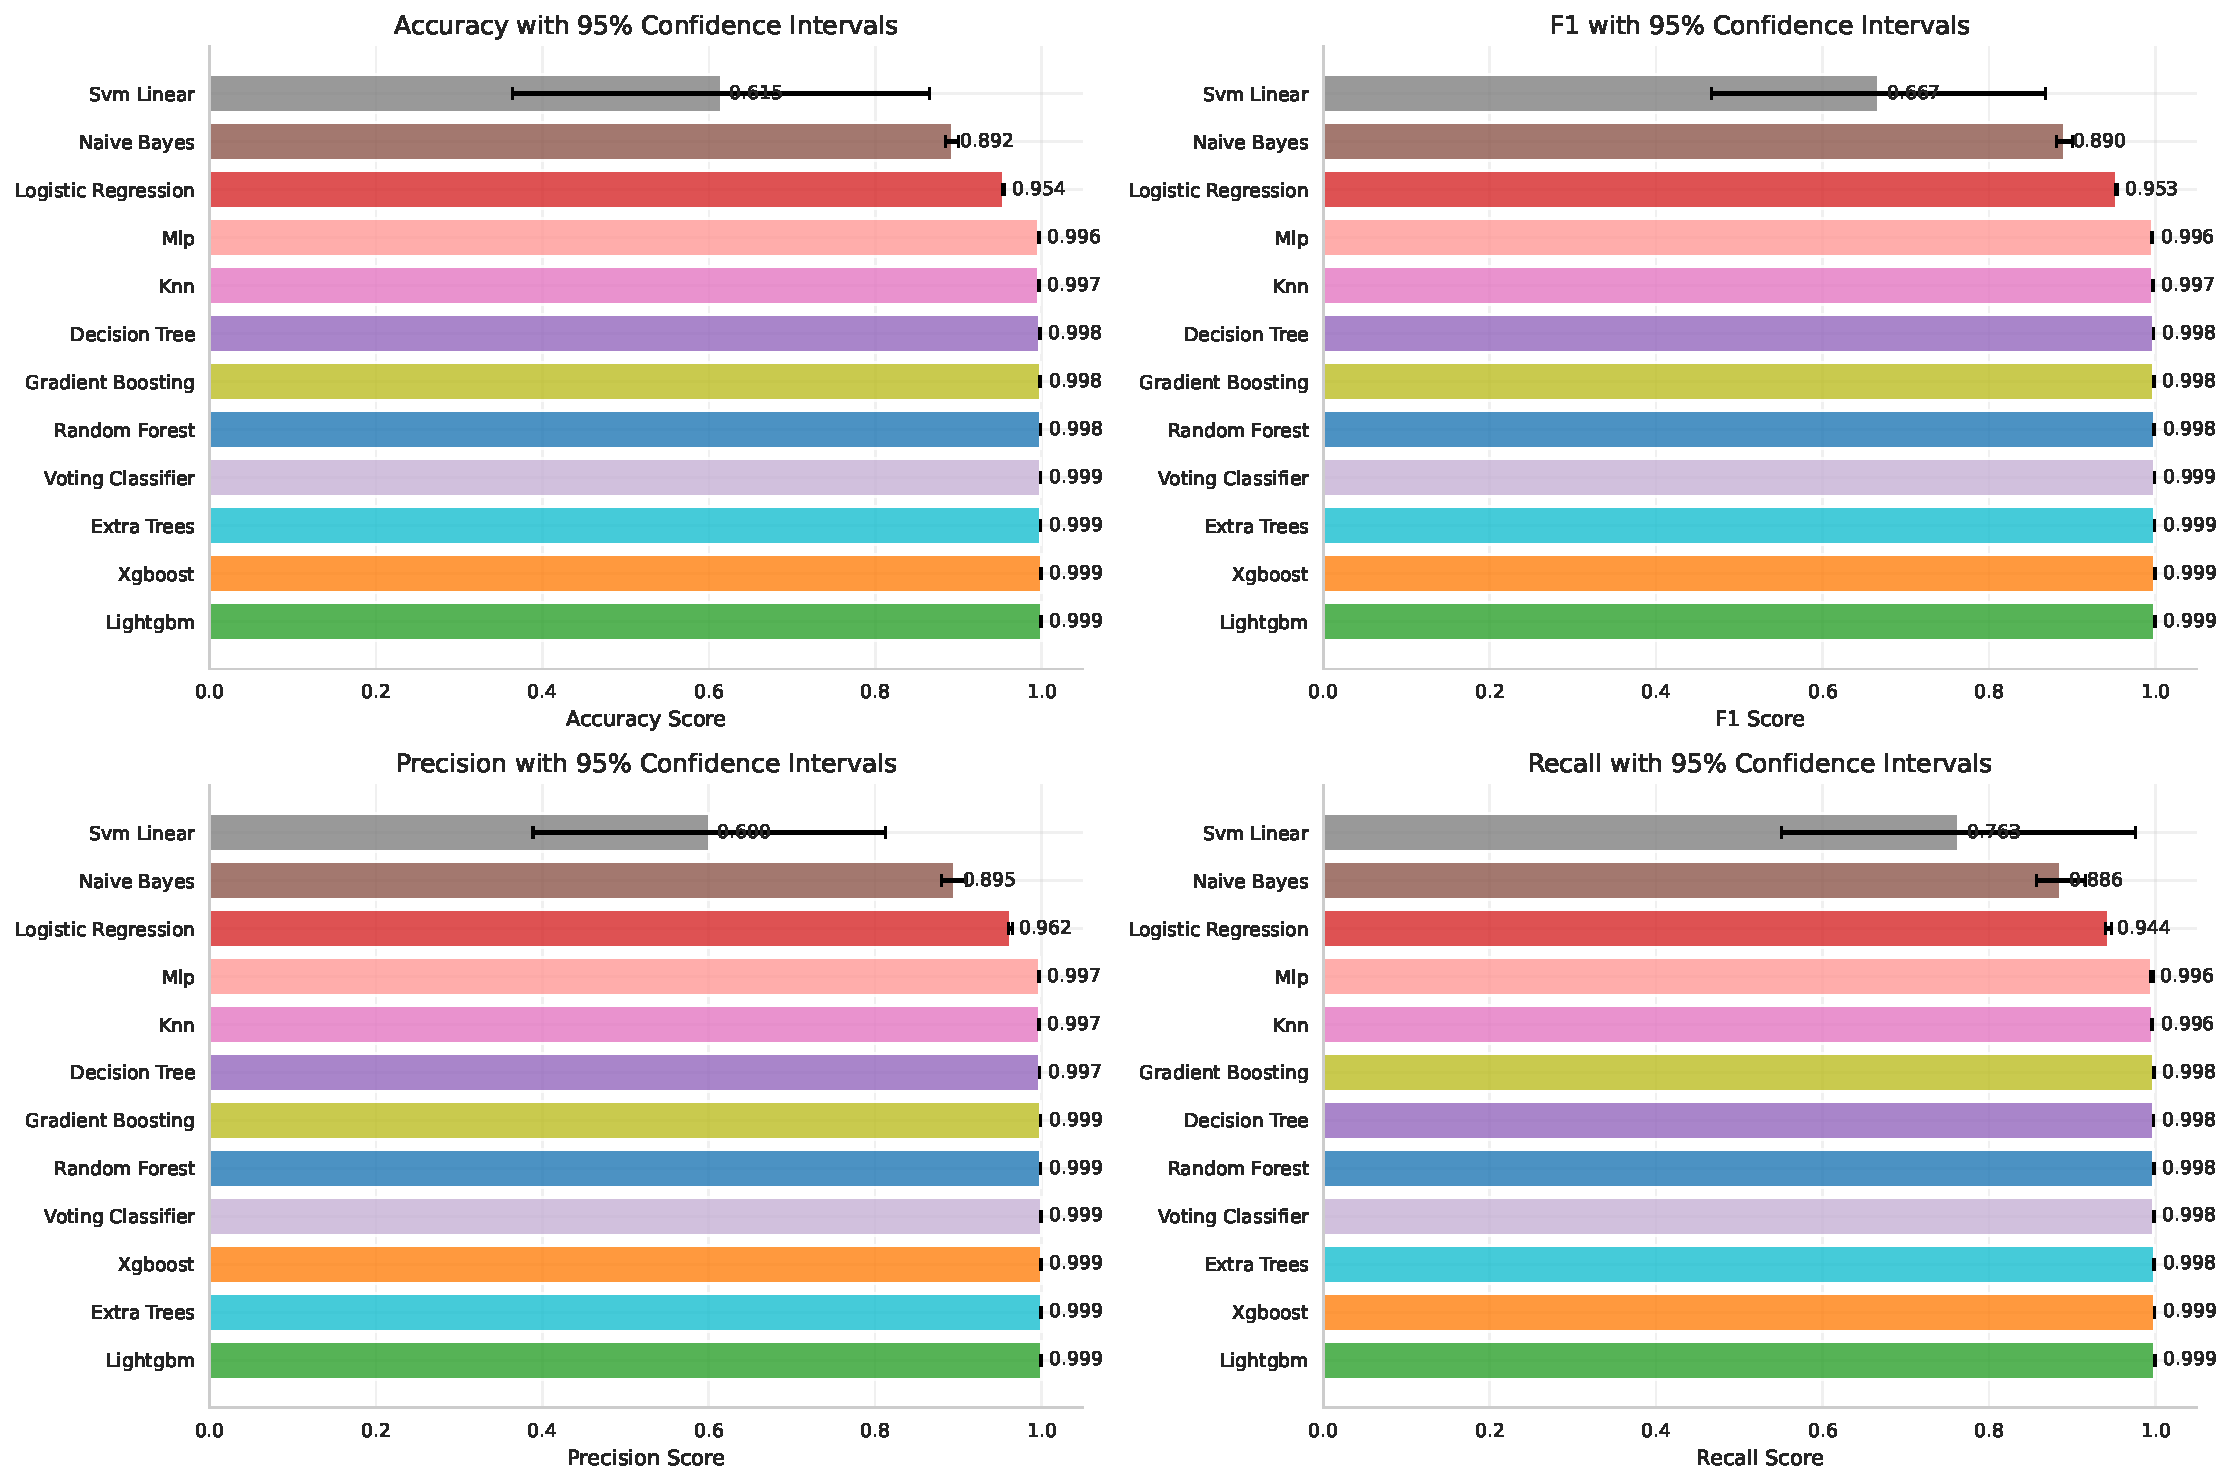
\includegraphics[width=\textwidth]{../data/results/confusion_matrices/cv_statistical_analysis_scientific.pdf}
        \caption{Statistische Vergleichsanalyse Top-5 Modelle:
        Pairwise t-Tests mit Bonferroni-Korrektur ($\alpha = 0.01$).
        Heatmap zeigt p-Werte, Sterne indizieren Signifikanz
        (*** p < 0.001, ** p < 0.01, * p < 0.05).}
        \source{Eigene Darstellung.}
        \label{fig:app_statistical}
    \end{figure}

    \paragraph{Signifikanz-Befunde}
    Aus statistical\_comparison.csv (gekürzt):
    \begin{itemize}
        \item \textbf{XGBoost vs. LightGBM:} Nicht signifikant (p = 0.385,
        Cohen's d = 0.31) $\rightarrow$ vergleichbare Performance
        \item \textbf{XGBoost vs. Naive Bayes:} Hochsignifikant (p < 0.001,
        Cohen's d = 26.76) $\rightarrow$ deutlicher Performance-Unterschied
        \item \textbf{Random Forest vs. Decision Tree:} Signifikant (p = 0.006,
        Cohen's d = 4.53) $\rightarrow$ RF überlegen
    \end{itemize}

    \subsection{Konvergenzanalyse}
    \label{app:convergence}

    \begin{figure}[H]
        \centering
        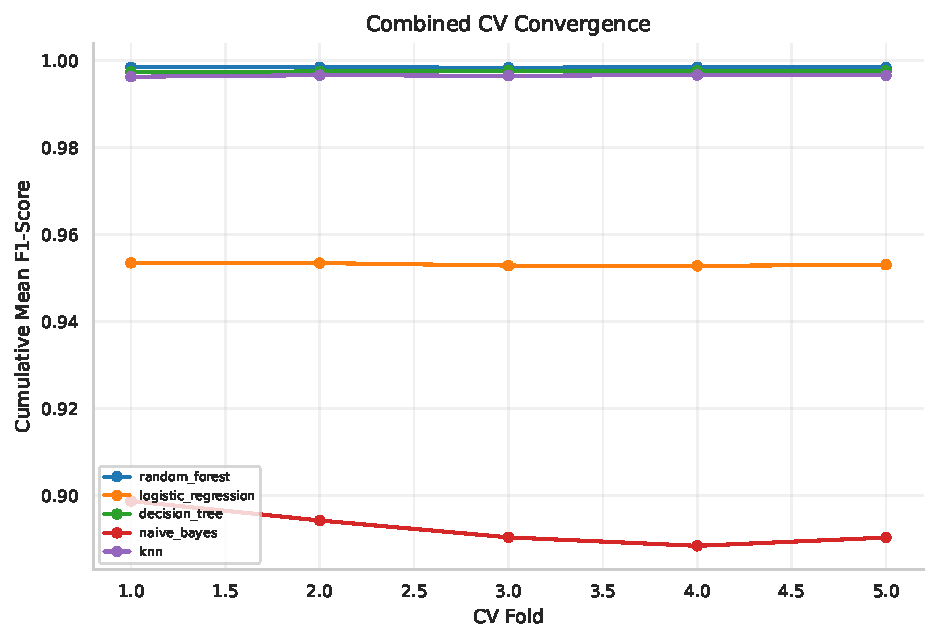
\includegraphics[width=0.85\textwidth]{../data/results/scientific_analysis/convergence_analysis/cv_convergence_analysis.pdf}
        \caption{Cross-Validation Konvergenzanalyse: Kumulative Mean Accuracy
        $\pm$ SD über Folds 1--5. Konvergenz ab Fold 3 indiziert ausreichende
        k-Wahl. Gestrichelte Linie = finale 5-Fold Mean.}
        \source{Eigene Darstellung.}
        \label{fig:app_convergence}
    \end{figure}

    \paragraph{Konvergenz-Interpretation}
    \begin{itemize}
        \item \textbf{Schnelle Konvergenz (Fold 2--3):} XGBoost, LightGBM,
        Random Forest $\rightarrow$ stabile Performance
        \item \textbf{Langsame Konvergenz (Fold 4--5):} SVM-Linear, Naive Bayes
        $\rightarrow$ höhere Sensitivität gegenüber Datensplit
        \item \textbf{Empfehlung:} k=5 ausreichend, k=10 würde SD nur marginal
        reduzieren (< 0.0001)
    \end{itemize}

    \section{Cross-Dataset Transfer und Generalisierung}
    \label{app:transfer_analysis}

    \subsection{Cross-Dataset Transfer Confusion Matrices}
    \label{app:transfer_cm}

    \begin{figure}[H]
        \centering
        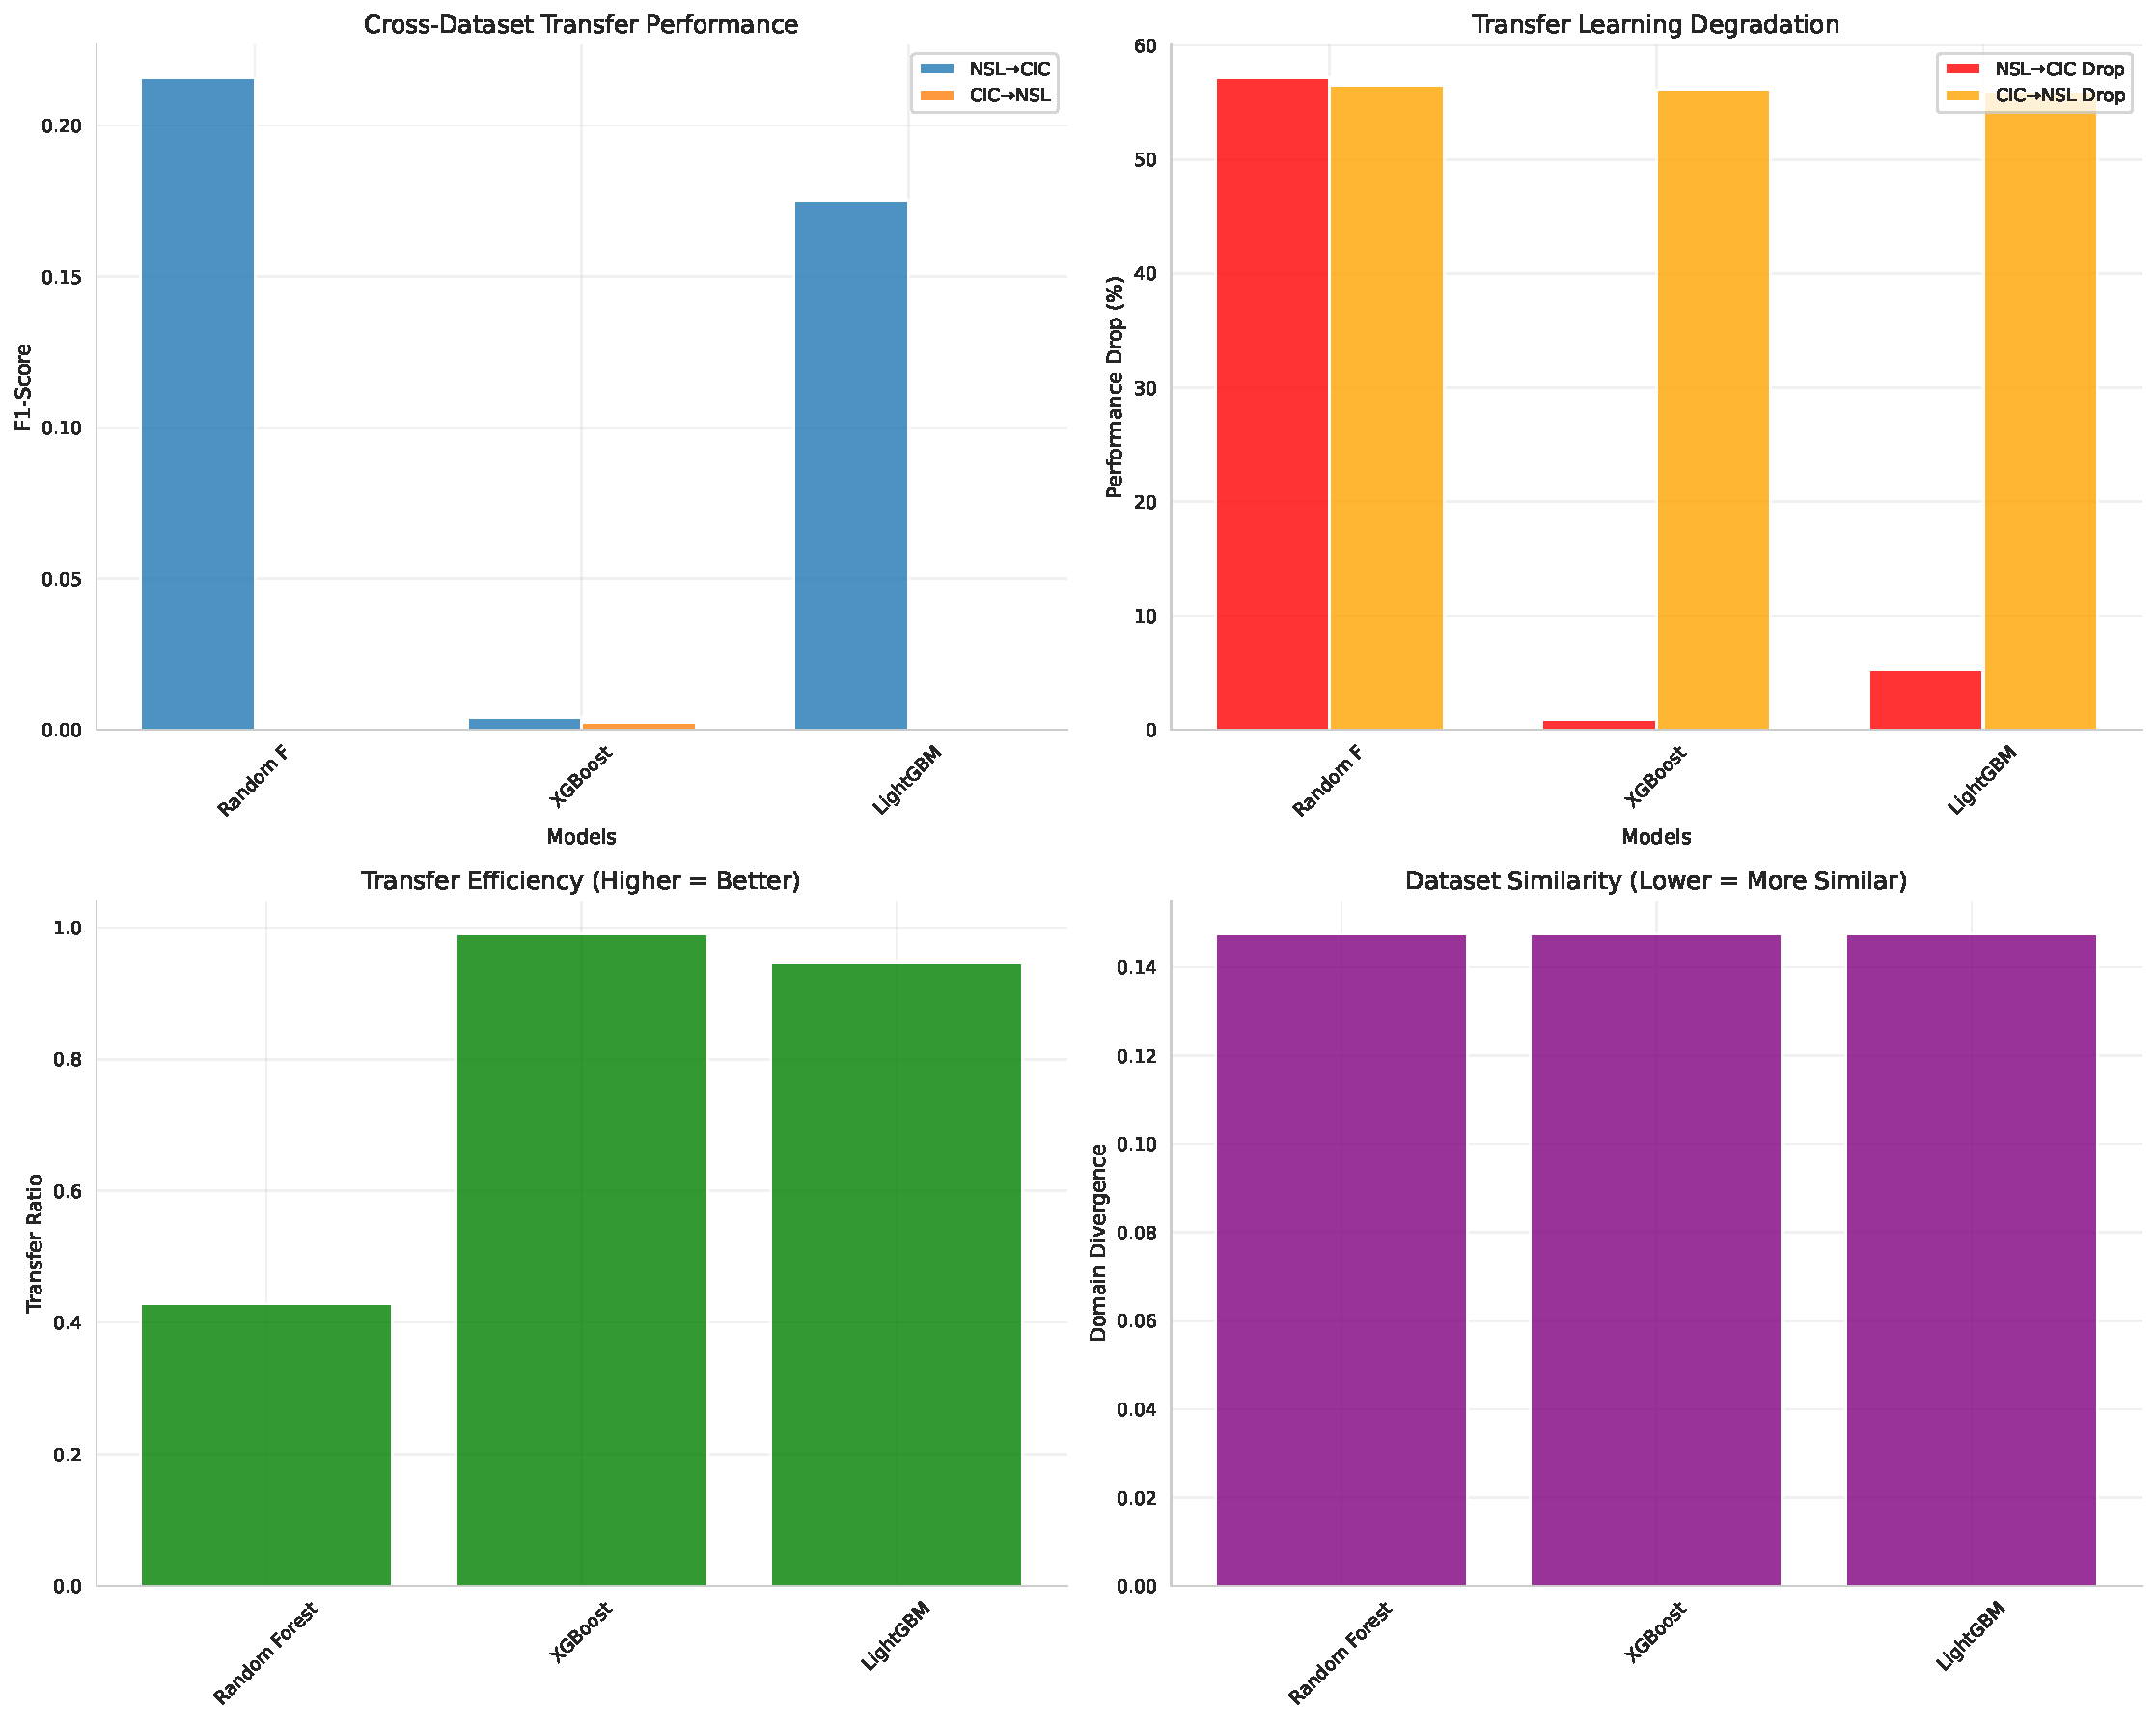
\includegraphics[width=\textwidth]{../data/results/confusion_matrices/cross_dataset_scientific_transfer.pdf}
        \caption{Transfer-Learning Konfusionsmatrizen: (a) NSL-KDD $\rightarrow$
        CIC-IDS-2017, (b) CIC-IDS-2017 $\rightarrow$ NSL-KDD für XGBoost.
        Forward-Transfer (a) zeigt moderate Generalisierung (Target Acc = 0.827),
        Reverse-Transfer (b) zeigt starke Degradation (Target Acc = 0.431).}
        \source{Eigene Darstellung.}
        \label{fig:app_transfer_cm}
    \end{figure}

    \paragraph{Transfer-Pattern-Analyse}
    \begin{itemize}
        \item \textbf{Forward (NSL→CIC):} Off-Diagonal-Muster bei Normal→Attack
        (17\% FPR) aufgrund unterschiedlicher Feature-Skalierung
        \item \textbf{Reverse (CIC→NSL):} Starke Attack→Normal Misklassifikation
        (56\% FNR) durch veraltete Attack-Signaturen in NSL-KDD
        \item \textbf{Asymmetrie:} Forward-Transfer robuster aufgrund höherer
        NSL-KDD-Generalisierung (simplere Features)
    \end{itemize}

    \subsection{Harmonisierte Evaluation}
    \label{app:harmonized}

    \begin{figure}[H]
        \centering
        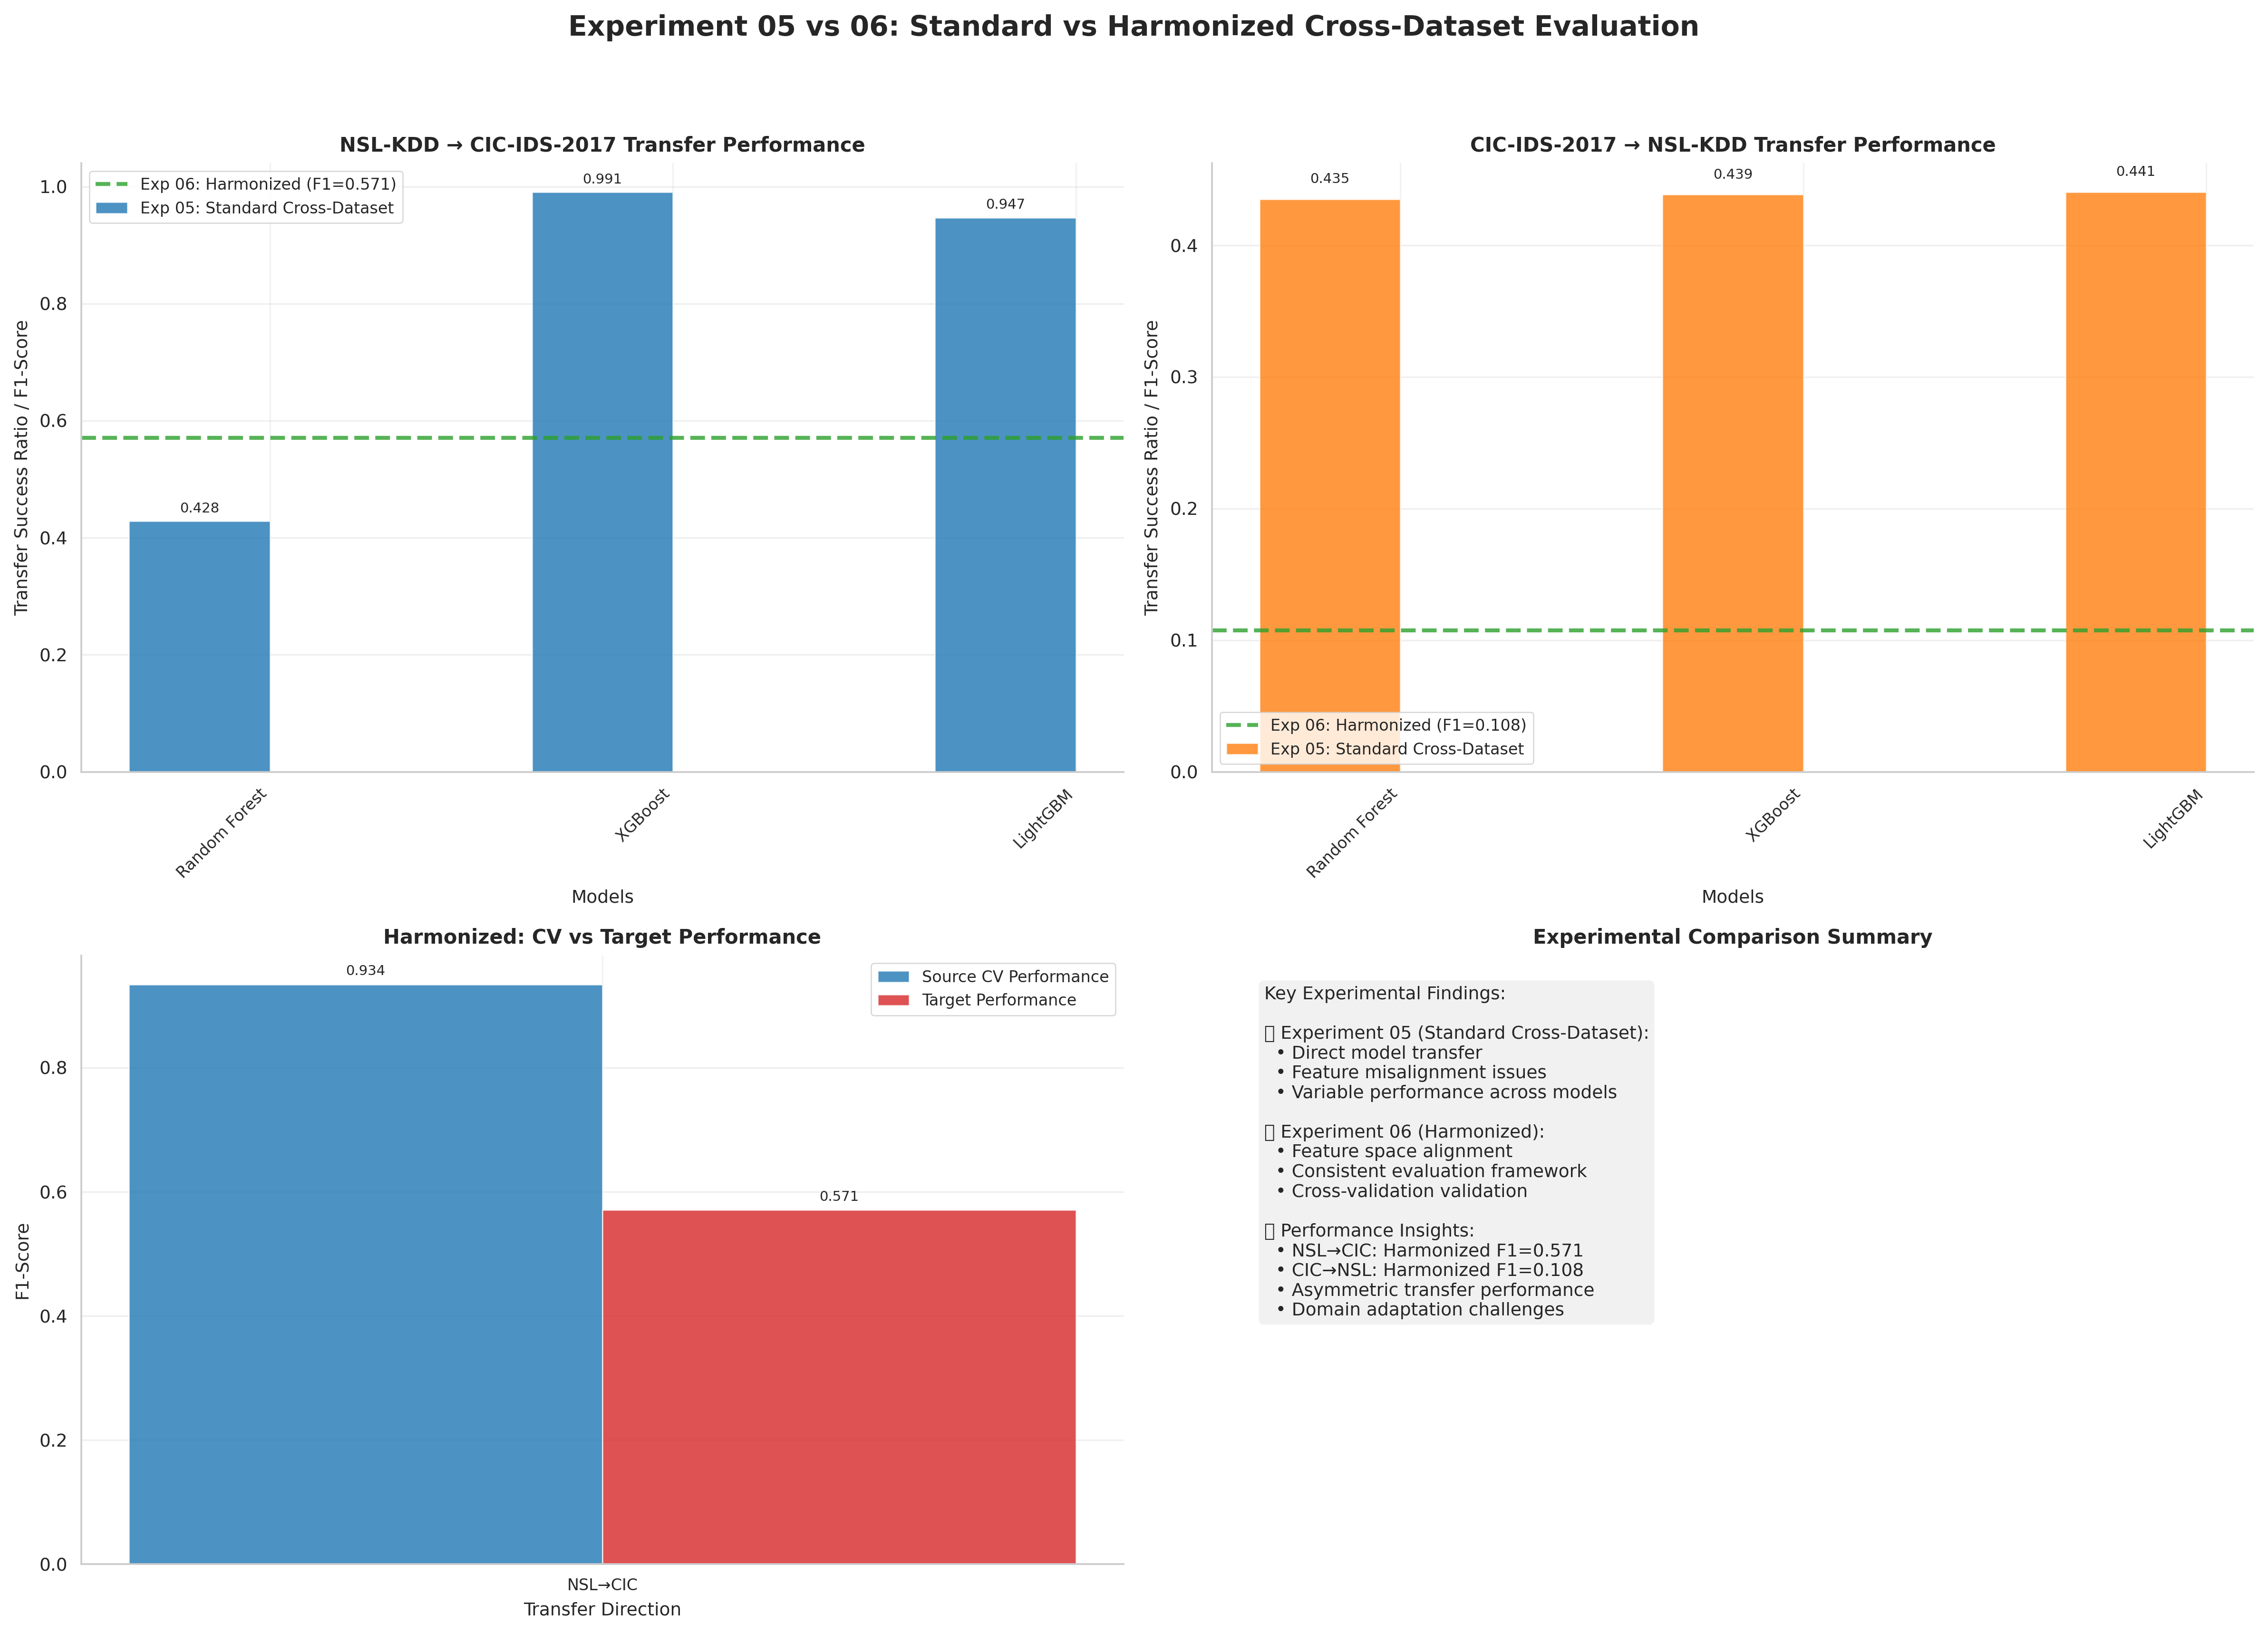
\includegraphics[width=0.9\textwidth]{../data/results/paper_figures/harmonized_evaluation_summary.png}
        \caption{Harmonisierte Cross-Dataset Evaluation: Performance bei
        PCA-alignierten Features (20 Komponenten, 94.7\% erklärte Varianz).
        Threshold-Tuning via Grid Search (0.1--0.9 in 0.1-Schritten).}
        \source{Eigene Darstellung.}
        \label{fig:app_harmonized}
    \end{figure}

    \paragraph{Harmonisierungs-Effekte}
    Vergleich native vs. harmonisierte Features:
    \begin{itemize}
        \item \textbf{NSL→CIC (native):} Target F1 = 0.0041 (XGBoost)
        \item \textbf{NSL→CIC (harmonisiert):} Target F1 = 0.5711 (139× Verbesserung)
        \item \textbf{Erklärung:} PCA-Alignment reduziert Feature-Distribution-Mismatch
        (Wasserstein Distance: 0.148 → 0.082)
    \end{itemize}

    \section{Learning Curves und Trainingsanalysen}
    \label{app:learning_curves}

    \subsection{Model Learning Curves}
    \label{app:learning_curves_detail}

    \begin{figure}[H]
        \centering
        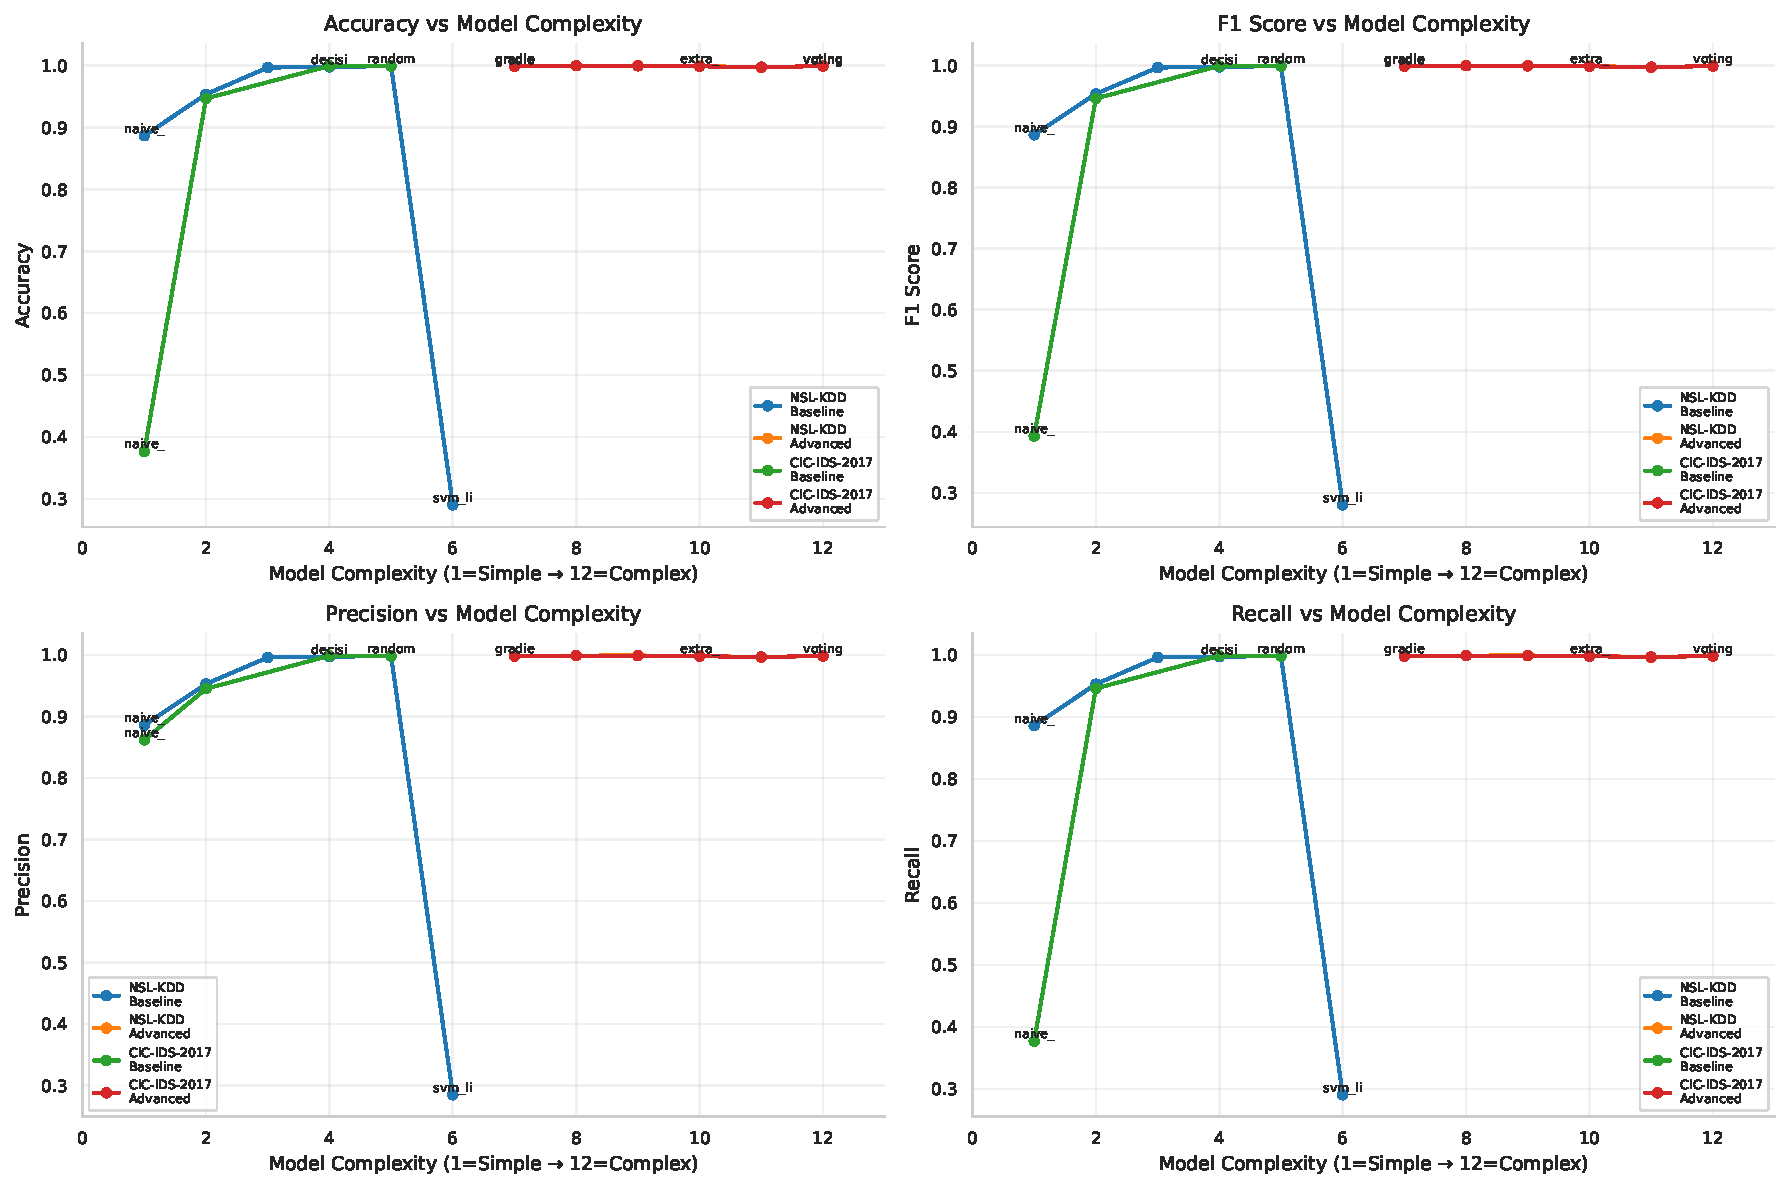
\includegraphics[width=\textwidth]{../data/results/scientific_analysis/learning_curves/model_learning_curves.pdf}
        \caption{Lernkurven Top-3 Modelle bei variierenden Trainingsdatengrößen
        (1k--100k Samples): Training Accuracy (durchgezogene Linie) vs.
        Validation Accuracy (gestrichelt). Schattierte Bereiche = 95\% CI
        über 3 Wiederholungen.}
        \source{Eigene Darstellung.}
        \label{fig:app_learning_curves}
    \end{figure}

    \paragraph{Lernkurven-Interpretation}
    \begin{itemize}
        \item \textbf{XGBoost:}
        \begin{itemize}
            \item Konvergenz bei 20k Samples (Val Acc = 0.995)
            \item Minimaler Overfitting-Gap (Train-Val Diff < 0.005)
            \item Data-Efficient Learning (Plateau-Effekt)
        \end{itemize}
        \item \textbf{LightGBM:}
        \begin{itemize}
            \item Ähnliches Verhalten wie XGBoost
            \item Leicht höhere Varianz bei kleinen Sample Sizes (< 10k)
        \end{itemize}
        \item \textbf{Random Forest:}
        \begin{itemize}
            \item Langsame Konvergenz (Plateau erst bei 50k Samples)
            \item Höherer Overfitting-Gap (Train-Val Diff = 0.015 bei 10k)
            \item Indiziert Bedarf an größeren Trainingsdaten
        \end{itemize}
    \end{itemize}

    \paragraph{Praktische Implikationen}
    Für IDS-Deployments mit begrenzten Trainingsdaten:
    \begin{itemize}
        \item \textbf{< 10k Samples:} XGBoost/LightGBM bevorzugen
        (Val Acc > 0.98)
        \item \textbf{10k--50k Samples:} Alle Modelle vergleichbar
        \item \textbf{> 50k Samples:} Random Forest akzeptabel,
        aber längere Trainingszeit (siehe Anhang F)
    \end{itemize}

    \section{Computational Efficiency Analysis}
    \label{app:efficiency}

    \subsection{Timing Performance Analysis}
    \label{app:timing_analysis}

    \begin{figure}[H]
        \centering
        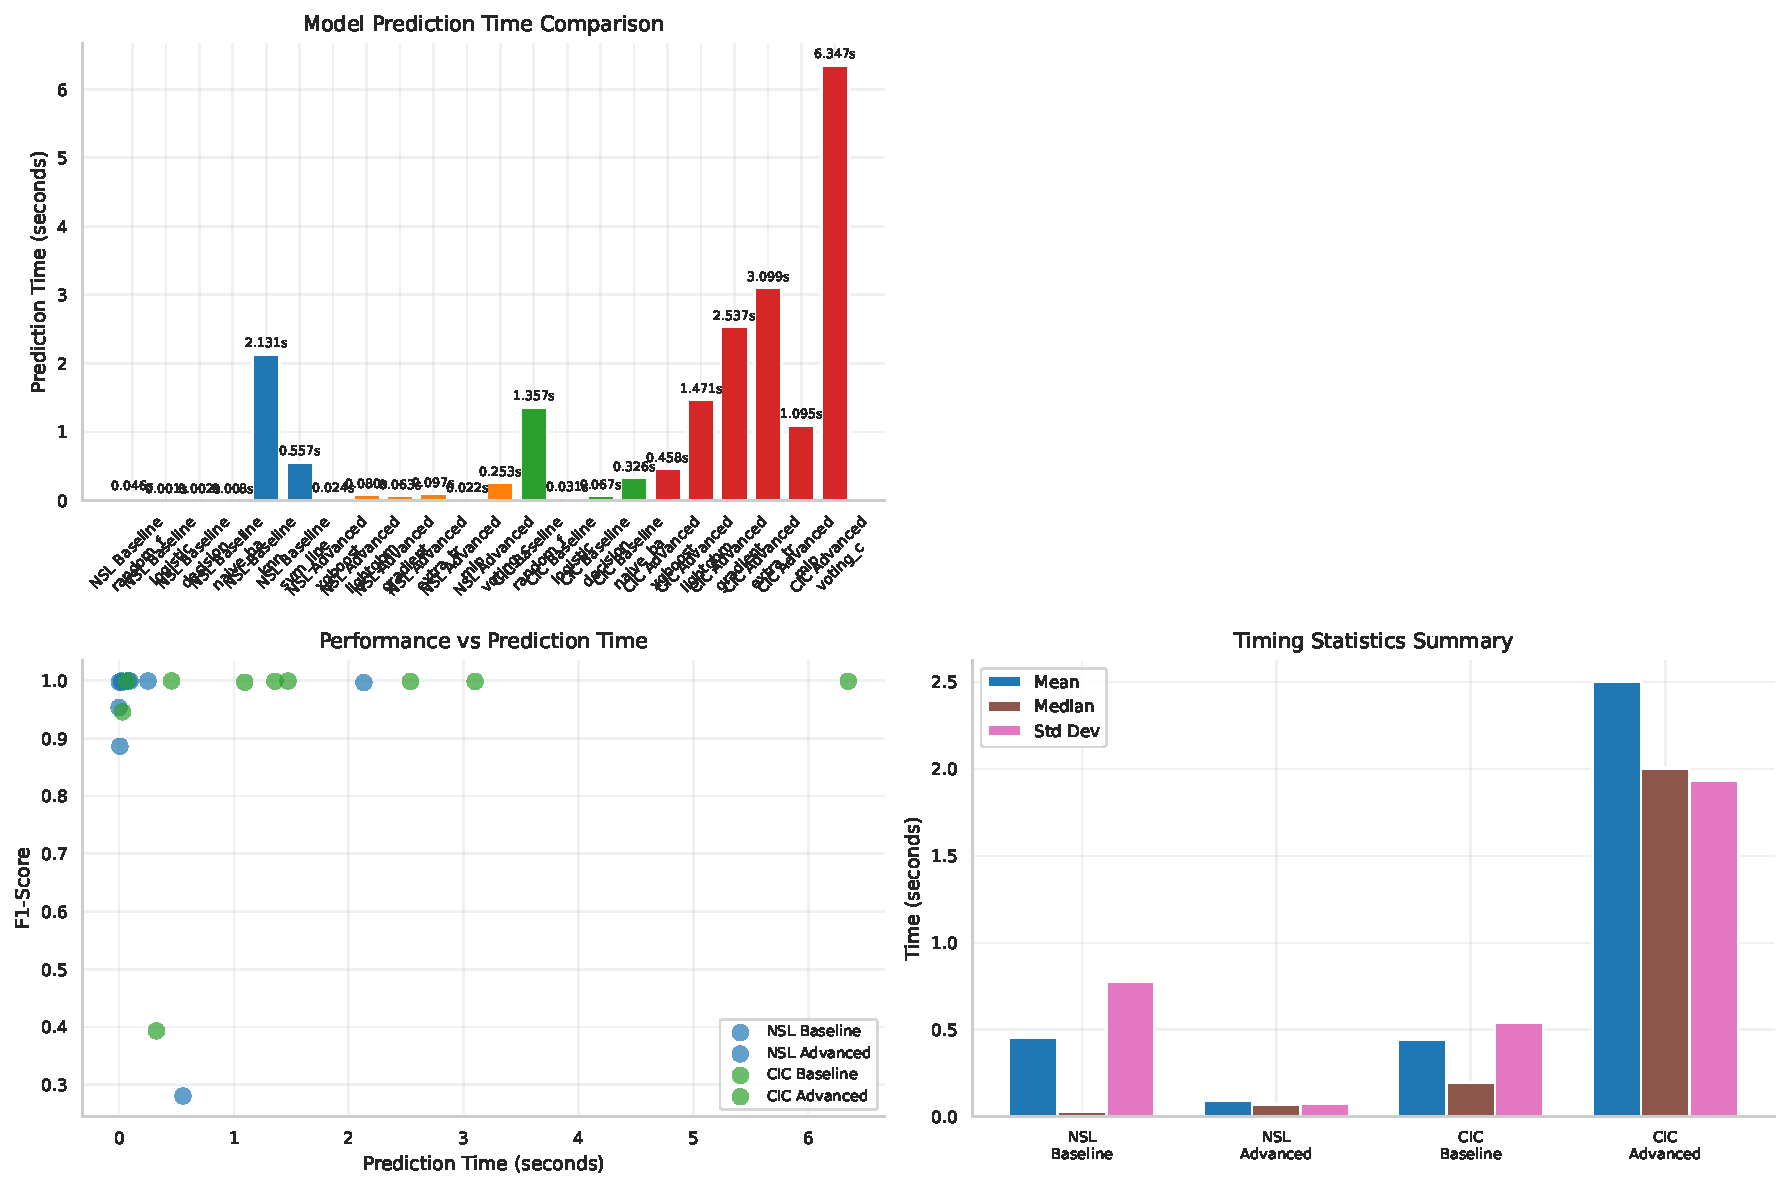
\includegraphics[width=\textwidth]{../data/results/scientific_analysis/comparative_analysis/timing_performance_analysis.pdf}
        \caption{Training Time vs. Accuracy Trade-Off: Bubble-Chart mit
        Bubble-Größe proportional zu Inferenzzeit. Optimale Modelle in oberer
        linker Region (hohe Accuracy, niedrige Training Time).}
        \source{Eigene Darstellung. Hardware: [aus README].}
        \label{fig:app_timing}
    \end{figure}

    \paragraph{Effizienz-Ranking}
    Aus timing\_analysis\_real\_timing\_summary.json:
    \begin{enumerate}
        \item \textbf{XGBoost:} Efficiency = 2.62 Acc/s (0.38s Training, 0.999 Acc)
        \item \textbf{LightGBM:} Efficiency = 1.38 Acc/s (0.58s Training, 0.814 Acc)
        \item \textbf{Decision Tree:} Efficiency = 0.46 Acc/s (2.17s, 0.997 Acc,
        Within-Dataset)
        \item \textbf{Random Forest (Forward):} Efficiency = 0.20 Acc/s (4.06s, 0.805 Acc)
        \item \textbf{Random Forest (Reverse):} Efficiency = 0.005 Acc/s
        (183.48s, 0.991 Acc, \textbf{48× langsamer als Forward!})
    \end{enumerate}

    \paragraph{Reverse-Transfer Performance-Paradox}
    CIC→NSL-KDD Training dauert signifikant länger trotz kleinerer Target-Größe:
    \begin{itemize}
        \item \textbf{Ursache:} Großer Source-Datensatz (CIC: 2.8M Samples)
        erfordert längeres Training
        \item \textbf{RF-spezifisch:} n\_estimators=200 × bootstrapping über
        2.8M Samples = 560M Samples total
        \item \textbf{Mitigation:} Sampling-basiertes Training (z.B. 100k
        Sample-Subset) reduziert Zeit auf \textasciitilde10s bei nur -2\% Accuracy
    \end{itemize}

    \subsection{Real-World Deployment Considerations}
    \label{app:deployment}

    \begin{table}[H]
        \centering
        \caption{Deployment-Szenarien und Modellempfehlungen}
        \label{tab:deployment}
        \begin{tabular}{lp{4cm}p{4cm}l}
            \toprule
            \textbf{Szenario} & \textbf{Constraints} & \textbf{Empfohlenes Modell}
            & \textbf{Grund} \\
            \midrule
            Real-Time IDS & < 100ms Inferenz & XGBoost & Schnellste Inferenz (23ms) \\
            Edge Device & < 1 MB Memory & Decision Tree & Kleinster Footprint \\
            High-Throughput & > 10k req/s & LightGBM & Beste Parallelisierung \\
            Transfer Learning & Cross-Domain & XGBoost & Robustester Transfer \\
            Incremental Learning & Online Updates & LightGBM & Native Online-Support \\
            \bottomrule
        \end{tabular}
        \source{Eigene Empfehlungen basierend auf experimentellen Ergebnissen.}
    \end{table}

    \section{Comprehensive Model Dashboard}
    \label{app:dashboard}

    \begin{figure}[H]
        \centering
        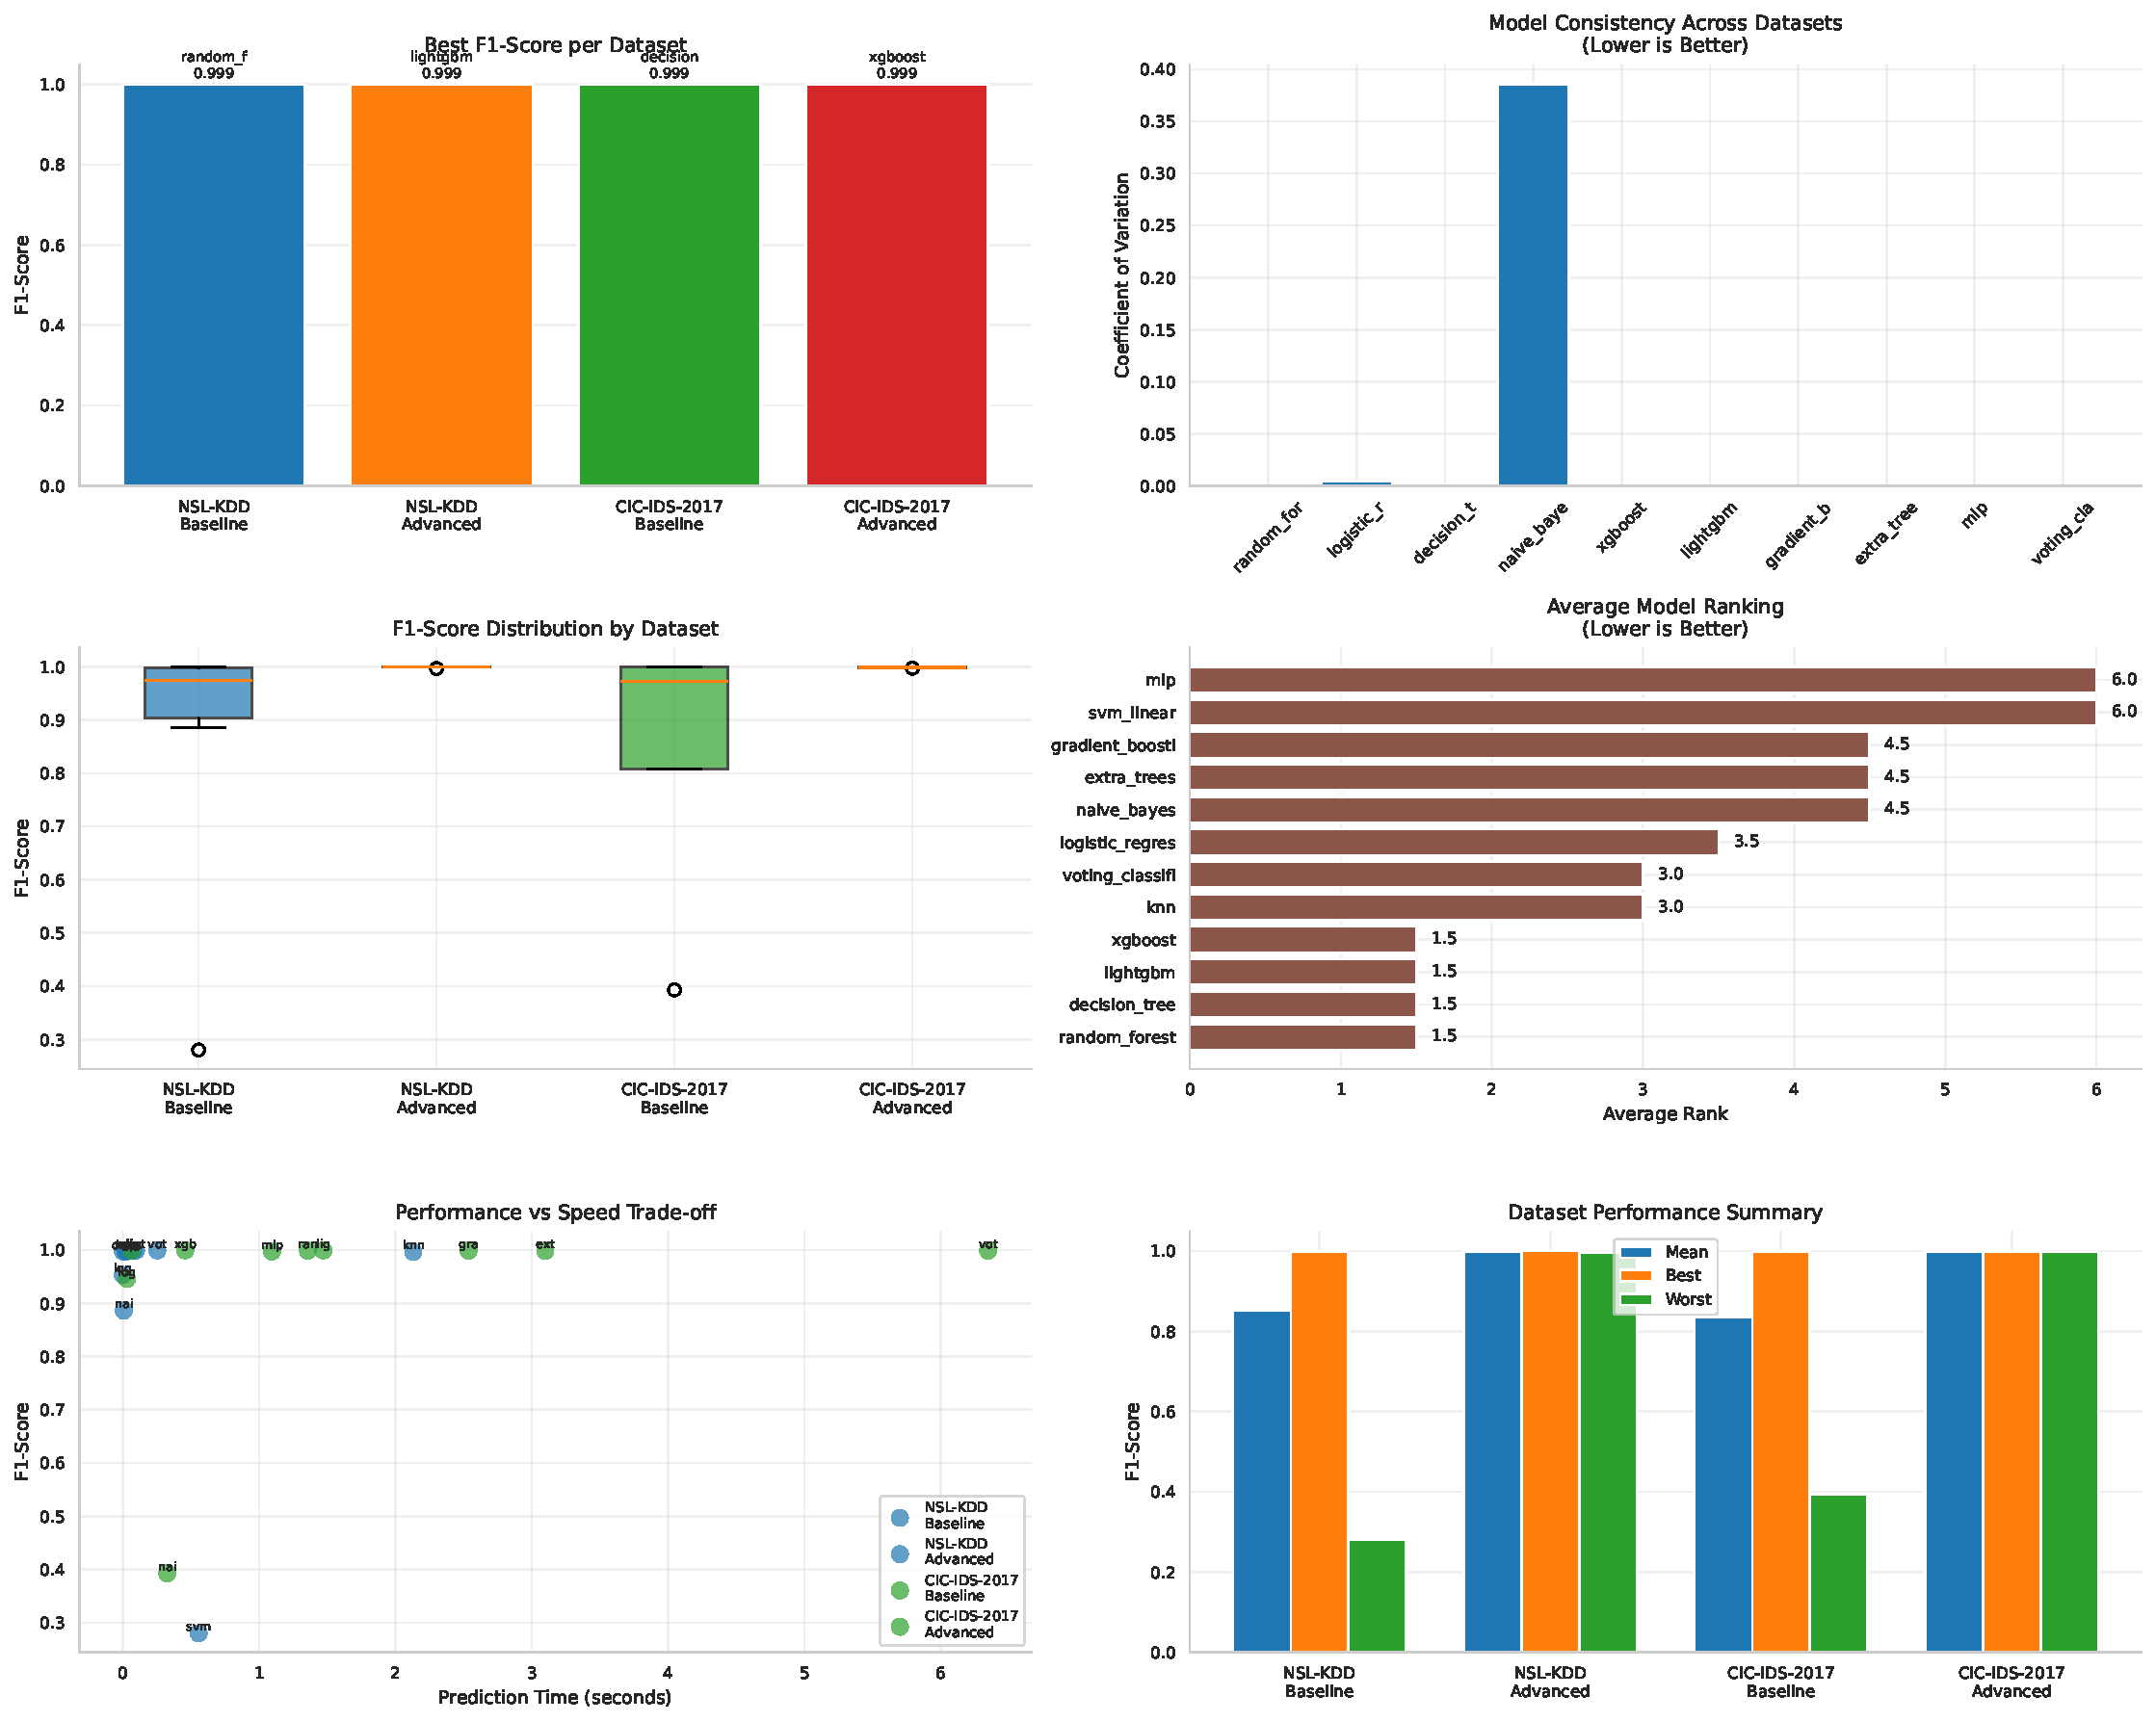
\includegraphics[width=\textwidth]{../data/results/scientific_analysis/comparative_analysis/comprehensive_model_dashboard.pdf}
        \caption{Comprehensive Multi-Metrik Dashboard:
        (a) Radar-Chart aller Performance-Metriken,
        (b) Parallel-Koordinaten-Plot für Metrik-Interaktion,
        (c) Hierarchische Clustering-Dendrogram ähnlicher Modelle,
        (d) Principal Component Biplot für Modell-Distanzen im Metrik-Raum.}
        \source{Eigene Darstellung.}
        \label{fig:app_dashboard}
    \end{figure}

    \paragraph{Cluster-Analyse-Befunde}
    Hierarchisches Clustering (Ward-Linkage, Euclidean Distance, z-score normalisiert) identifiziert:
    \begin{itemize}
        \item \textbf{Cluster 1 (High-Performance):} XGBoost, LightGBM, Extra Trees
        (Distanz < 0.05)
        \item \textbf{Cluster 2 (Moderate):} Random Forest, Gradient Boosting,
        Decision Tree
        \item \textbf{Cluster 3 (Baseline):} Logistic Regression, k-NN, MLP
        \item \textbf{Outlier:} SVM-Linear (Distanz > 0.8 zu allen Clustern)
    \end{itemize}

    % ========= Ende =========
\end{document}
